\documentclass[twoside,single,12pt]{lion-msc}

\title{Resolved spectroscopy of planet forming disks with SPHERE/IFS}
\author{Ardjan Sturm}

\affiliation{Huygens-Kamerlingh Onnes Laboratory, Leiden University}   % this is the default value
%\affiliation{Instituut-Lorentz, Leiden University}                     % for theoretical physics

%\affiliation{Huygens-Kamerlingh Onnes Laboratorium, Universiteit Leiden}   % experimental physics in Dutch
%\affiliation{Instituut-Lorentz, Universiteit Leiden}                       % theoretical physics in Dutch

\address{P.O. Box 9500, 2300 RA Leiden, The Netherlands}               % default address - uncomment if need be

%\newdate{date}{\day}{\month}{\year}           % definition of time and date using datetime package
%\newdate{date}{27}{08}{2010}
%\date{\displaydate{date}}

\studentid{S1663011}                           % check you student ID, LaTeX does not do this
\abstract{\noindent\textit{Context.} Much SPHERE/IFS data of circumstellar disks is yet unpublished, since this data is always collected in parallel with IRDIS, which is much easier to reduce and analyze.\\
\textit{Aims.} We search for a good and reliable way to reduce raw IFS data and study the effects of different post-processing methods on the morphology of protoplanetary disks.\\
\textit{Methods.} We used the common pipeline of ESO to reduce spatially resolved spectral IFS data (YJ band) of RXJ1615.3-3255 and applied classical ADI, classical SDI and classical RDI on the data.\\
\textit{Results.} We detected a ring, an arc and an inner disk component in both the ADI and SDI image, the ring is detected in the RDI image as well. We conclude that we can trust the SDI data the best around the minor axis of the ring since ADI and RDI have to deal with self-subtraction and over subtraction in that region, the other parts of the ring can be trusted the best in the ADI and RDI data. The disk signal appears to be red, but further research is needed to conclude whether this effect is astrophysical or not. \\
}     % limit your self to 1/2 page or 500 words
\supervisor{Dr. M.A. Kenworthy}                         % Note that this should be a LION staff member!
\corrector{Prof. dr. J.M. van Ruitenbeek}                      % This could be a LION staff member or your external supervisor

%\degree{Master of Science}                     % The default option is "Bachelor of Science", change if needed

\major{Physics and Astronomy}                  % The default option is "Physics", change if needed
%\major{Physics and Mathematics}

% optional cover picture - should be jpg or pdf
\coverpicture{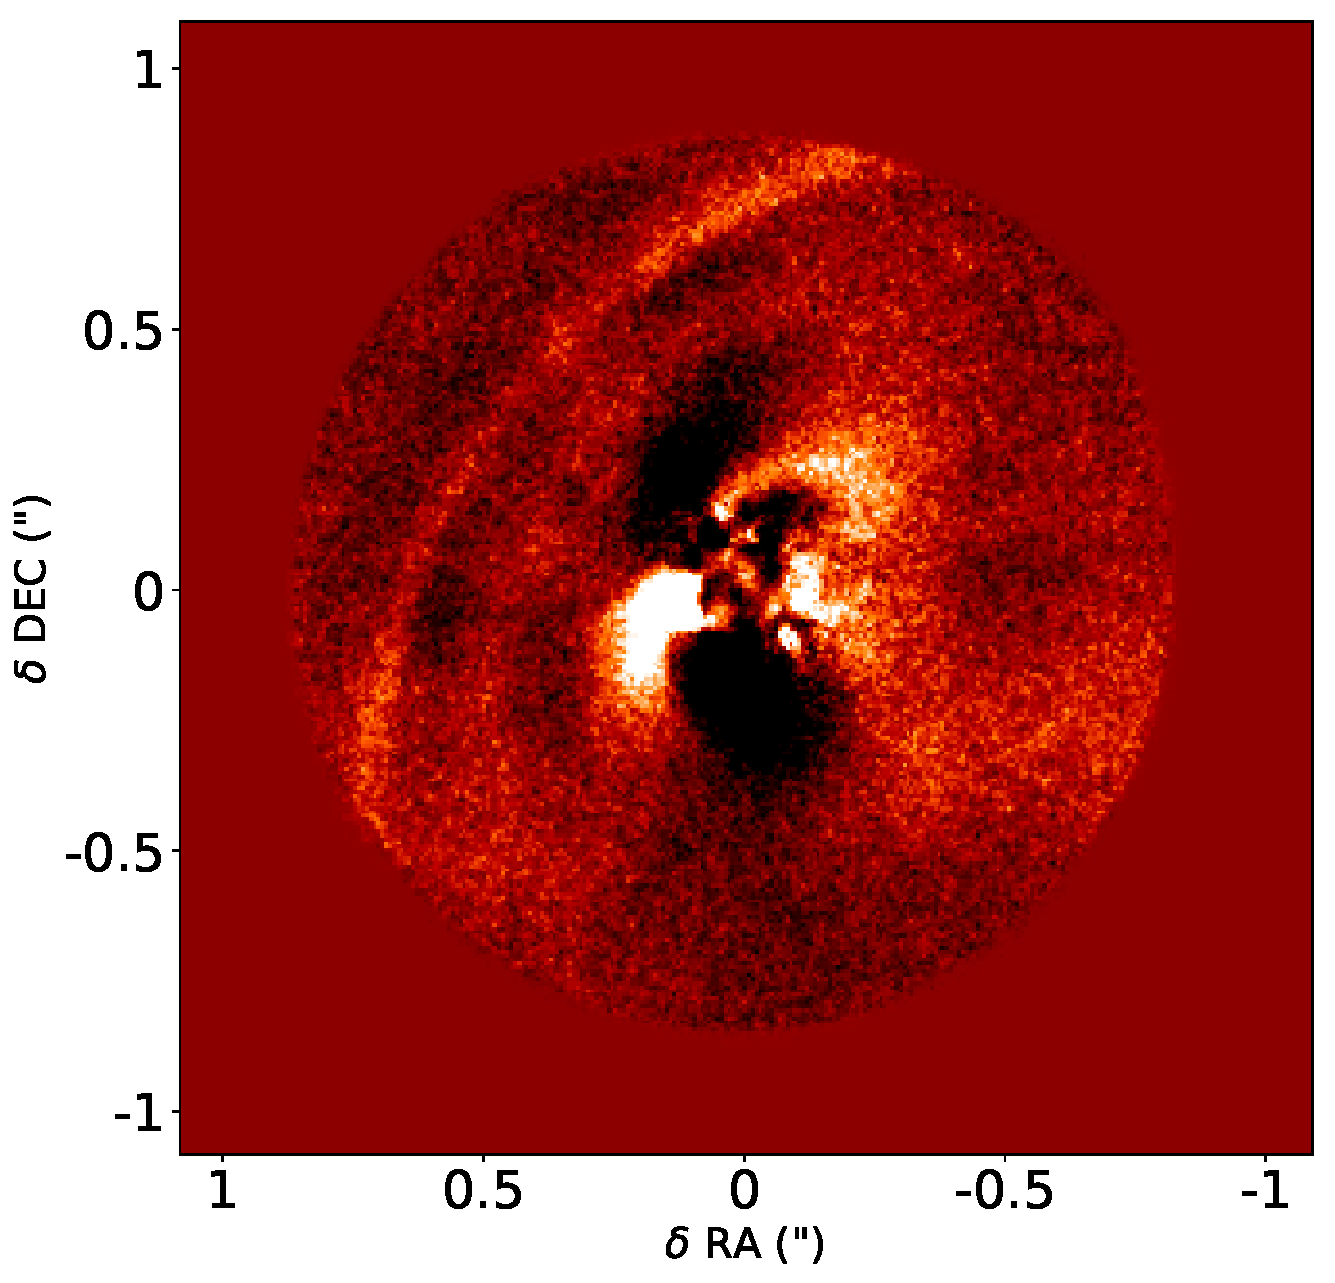
\includegraphics[trim={4.3cm 4cm 2.3cm 2cm},clip,width=6cm]{ADI_tot}}

% Use this to make hyperlinks visible in the document.
% \hypersetup{colorlinks=true}

% ---------------------------------------------------------------- My definitions!
% \renewcommand{\vec}[1] {\ensuremath{ \overrightarrow{ #1 } }}
\renewcommand{\vec}[1] {\ensuremath{ \mathbf{ #1 } }}
% \bra \ket \braket and \proj
\newcommand{\bra}[1]{\ensuremath{\langle #1 \vert}}
\newcommand{\ket}[1]{\ensuremath{\vert #1 \rangle}}
\newcommand{\braket}[2]{\ensuremath{\langle #1 \vert #2 \rangle}}
\newcommand{\proj}[1]{\ensuremath{\vert #1 \rangle \langle #1 \vert}}

\newcommand{\kpar}{\ensuremath{k_\parallel}}
% ----------------------------------------------------------------

% \usepackage{tocloft}
% \renewcommand{\cftchapdotsep}{\cftdotsep}
\usepackage{subcaption}
\usepackage{makecell,tabularx}
\usepackage{longtable}
\usepackage{graphicx,wrapfig,lipsum}
\usepackage{caption}
\usepackage[skip=10pt]{subcaption}
\usepackage{mdframed}
\usepackage{rotating}
%\captionsetup[subfigure]{skip=25pt} % global setting for subfigure

\begin{document}

% roman numbering in the table of contents section
\pagenumbering{roman}

\maketitle

% Table of contents :  it is a good idea to include this into your thesis
\tableofcontents
\cleardoublepage

% The following list of figures and list of tables are optional. Remove the comments if needed
%\listoffigures
%\newpage

%\listoftables
%\newpage

% in the main part of the document use standard arabic numbers. Page counter resets to 1.
\pagenumbering{arabic}
\chapter{Introduction}
One of the biggest questions that arises in every single human mind is how the world around us is formed. Even young children find it intriguing that a pea grows to a complete plant and that their parents were once children. Much research in astronomy is about how the universe has taken his shape it has today. How do galaxies, stars and ultimately planets form? It has been a question for a long time, scientists have been asking the question if the solar system was the only place in the universe where planets exist. Since then, many indirect methods have been developed that could tell if a star hosted planets and the first exoplanet was soon confirmed \cite{Mayor1995}.
\bigskip

Scientists have made huge progress in the last few decades in understanding the formation of stars and planets. It is now common knowledge that stars are formed by the collapse of a cloud of gas and dust. The gas and dust that is left in the cloud after the birth of a star starts to fall inwards and starts to orbit the star in a plane due to conservation of angular momentum, forming an accretion disk. In this accretion disk planets start to form when grains stick together to form pebbles, pebbles form planetessimals and planetessimals form planets. Another possibility is that the disk gets gravitationally unstable, the disk starts to fragment and gas giant planets are formed \cite{Armitage2010}.
\bigskip

Direct imaging of planets and disks has been impossible for a long time, since the contrast between stars and planets is too big and the point spread function (PSF) of the star too much extended. With the development of special optics called coronagraphs that improve the contrast, special adaptive optics system that corrects for the distortion of the light in the atmosphere and special techniques to reduce the stellar PSF, we are now able to image planets and protoplanetary disks directly. This provides detailed information of the conditions in different planetary systems and protoplanetary disks, which improves the understanding of the formation of planetary systems.
\bigskip

SPHERE (Spectro-Polarimetric High-contrast Exoplanets REsearch \citep{Beuzit2008}), one of the instruments of the Very Large Telescopes (VLT) in Chile, was build for direct imaging of planets. This instrument collects, amongst other things, high resolution data of exoplanets and circumstellar disks. One mode of the subsystems of the instrument gives light in parallel to both IRDIS and IFS. IRDIS (InfraRed Dual Imaging and Spectograph \cite{Dohlen2008}) is a subsystem that provides classical imaging, dual band imaging, dual-polarization imaging and long slit spectroscopy with a good resolving power. IFS (Integral Field spectrograph \citep{Claudi2006}) is a subsystem that provides a spatially resolved spectrum over the Y-J or Y-H range. Since IRDIS data is easier to reduce and to analyze, and the field of view (FOV) of IRDIS is much bigger than the FOV of the IFS, IRDIS data is much more often analyzed than IFS data. Thus much of the disk data taken by IFS is still unpublished.
\bigskip

Since the IFS provides a spatially resolved spectrum of an object, it is possible to get a spectrum of a protoplanetary disk. Until now, we do not have detailed information about the color of the object that mainly will be analyzed in this project, the T-Tauri star RX J1615.3-3255. Reliable spectral information of protoplanetary disks can lead to a better understanding of ongoing planet formation in protoplanetary disks in general, since resolved spectral data of a disk can tell something about the local grain properties throughout the disk.
\bigskip

Many steps are neccessary to recover a spectrum of the disk out of raw data. One of the first steps is a good reduction of the data. Hence, one of the main goals of this research is to investigate what is the best way to reduce the raw data: what calibration data is needed and which calibration steps have to be taken. There are various effects at play that we want to understand once this basic reduction is done. It appears that the disk is detected more easily at longer wavelengths. One of the goals of the project is to check if this is the case for more disks, which could indicate that it is something astrophysical, or that this is only an effect of the adaptive optic's performance getting better at longer wavelengths, which it generally does. The starlight can be subtracted by use of different post-processing techniques in order to detect the disk. These techniques can affect the spectrum and the morphology of the disk. Another goal of the project is therefore to check how strong these effects are and when we can trust an extracted spectrum.
\bigskip

\chapter{Theory}
\section{Protoplanetary disks}
\begin{wrapfigure}{R}{0.35\textwidth}
\vspace{-3mm}
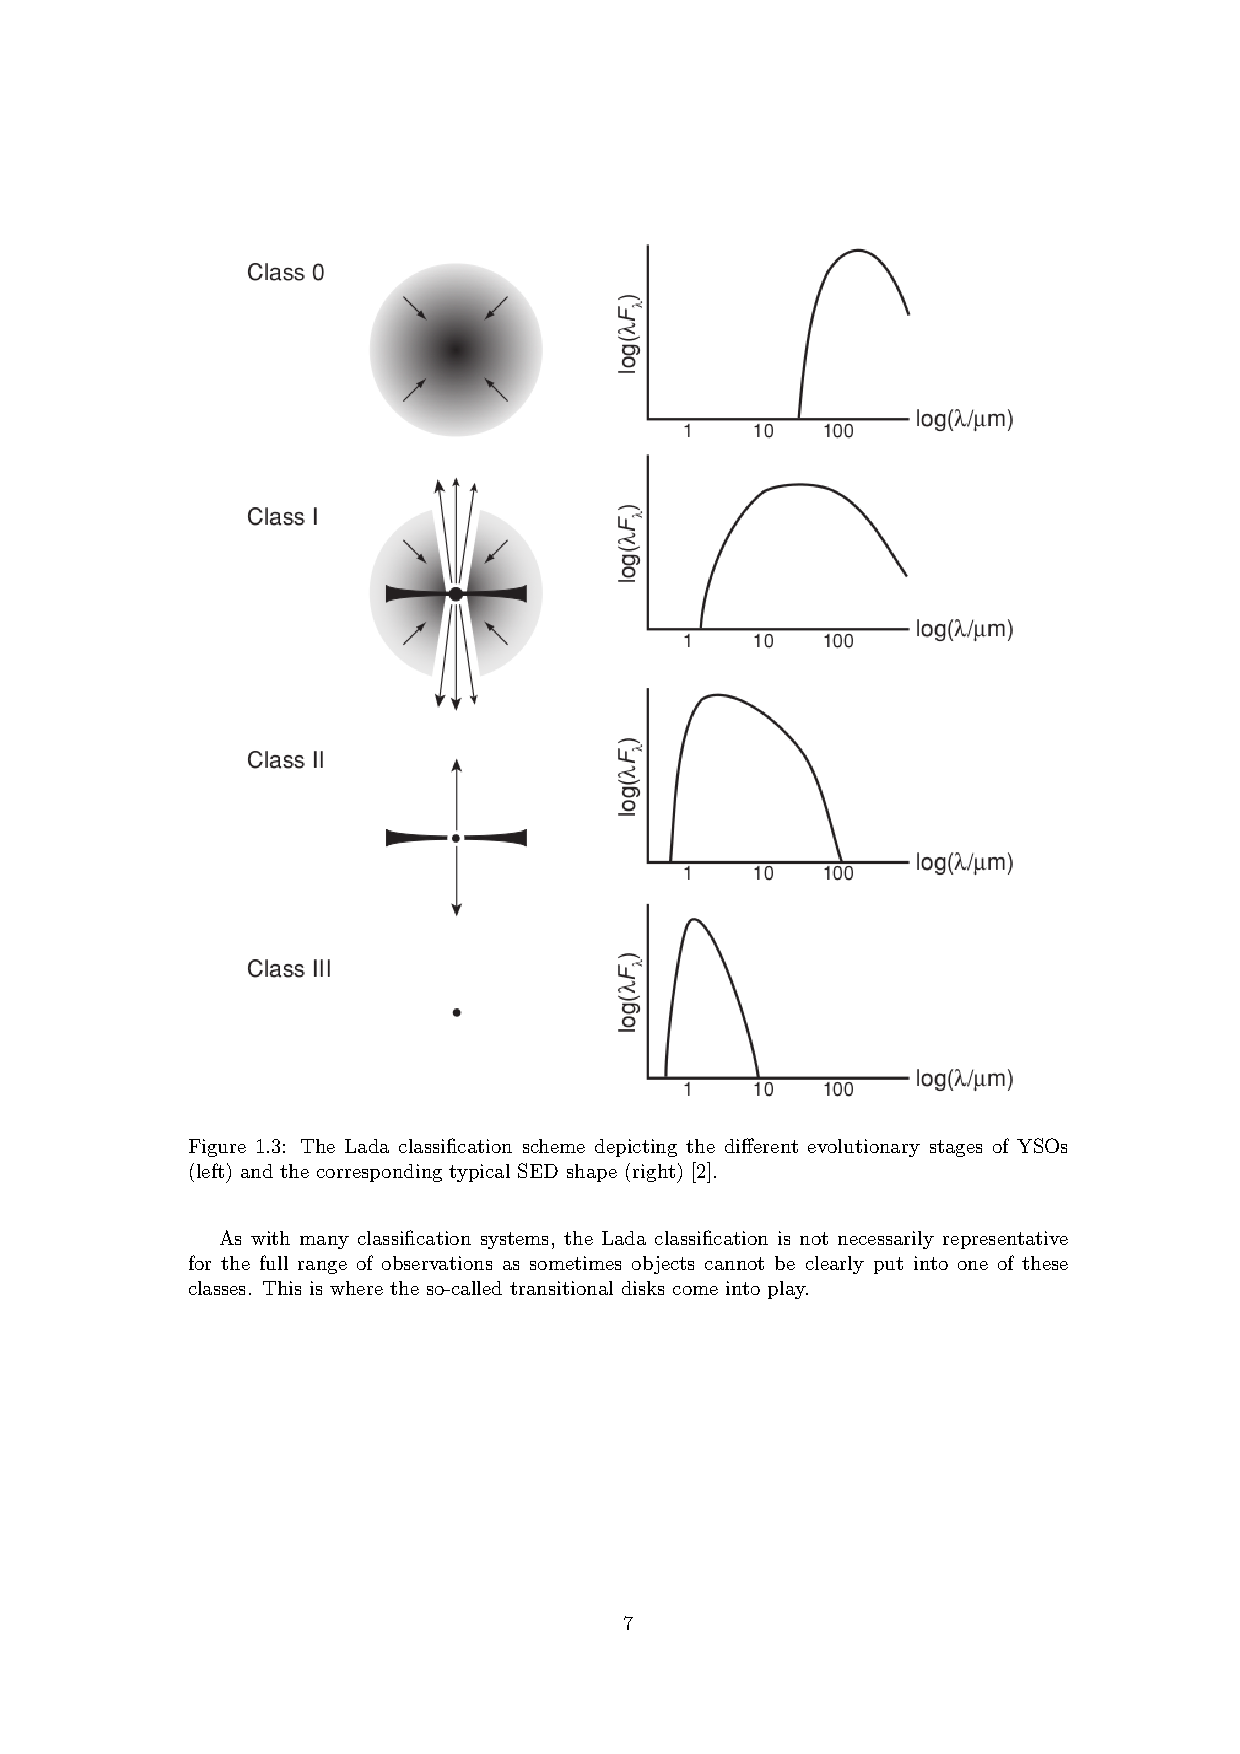
\includegraphics[trim={4cm 11cm 11cm 4cm},clip,width = 0.35\textwidth]{classscheme}
\caption{The four classes of young stellar objects (YSO), from top to bottom: a cloud collapses into a protostar (Class 0), a disk starts to form by conservation of angular momentum (Class I), the outer envelope dissipates, the protostar is only surrounded by a disk (Class II), the disk gets optically thin and a star with possibly a planetary system is left (Class III). Figure adapted from\citep{Armitage2010}}
\vspace{-65pt}
\label{fig:classscheme}
\end{wrapfigure}%

The formation of a star with a planetary system like the sun has multiple stages.  The evolution of protoplanetary disks is classified in four different classes, according to the scheme that Lada introduced in 1987\cite{Lada1987} as illustrated in Figure \ref{fig:classscheme}. This classification is based on the slope of the spectral energy distribution (SED) of young stellar objects in the mid-infrared.
\bigskip

The youngest stars are found in Class 0. They have a massive accretion disk that is indistinct from the dense envelope. All the visible light of the protostar is absorbed by this accreting envelope, making these objects invisible in the optical. At first these objects were no part of the classification because they were first discovered until decades later when the first infrared and millimeter telescopes were built.
\bigskip

The objects in Class 1 have a distinct disk and get more visible in the optical, since the star in the center is less obscured by the decreasing density of the envelope. Since the density in the disk increases, the temperature rises and the peak of the emission of the disk starts shifting to the mid-IR. Objects in this class could also eject collimated jets at a high velocity from the poles. These jets are formed as a byproduct of the accretion process and could influence the evolutionary track of the object.
\bigskip

The envelope is totally dissipated for Class 2 objects and the star is only surrounded by an optically thick accretion disk. These objects are also known as T-Tauri stars, named after the prototype T-Tauri, if they have a mass smaller than 2 $M_\odot$. These objects are all younger than 10 million years. Analogs of these stars, but with a mass higher than 2 $M_\odot$ are called Herbig Ae/Be stars. 
\bigskip

The gas in the disk of Class 3 objects has dissipated, leaving the protostar with an optically thin debris disk and a possible planetary system. The SED no longer contains a disk component at longer wavelengths, but is totally dominated by the light of the protostar. This class ends when the nuclear fusion in the core of the protostar starts and the protostar becomes a main sequence star.
\bigskip

Objects in the stage between Class 2 and Class 3 are called transition disks. These stars  have more than just a debris disk, but the disk starts to get less prominent. Some disks have a cleared cavity, close to the star, since this part is heated the most by the star. Inside the cleared region an inner disk can be present as a remnant from the optically thick accretion disk.

\section{The object}
The main object of this study is the T-Tauri star RX J1615.3-3255 (hereafter RX J1615). RX J1615 is a star in the scorpius constellation on the southern hemisphere, with coordinates 16 15 20.231 -32 55 05.10 and a member of the Lupus star forming region. The distance to this region is estimated to be 158 pc \cite{Gaia2018}. The mass of RX J1615 is previously determined to be 1.1 $M_\odot$ and the age 1.4 Myr \cite{Wahhaj2010}. The spectral type of RX J1615 is K5D with an R-band magnitude of 11.21 \cite{Krautter1997}. It is well known that this star hosts large circumstellar disk structures. As illustrated in Figure \ref{fig:irdisjos}, there are two different rings detected in IRDIS data (R1 and R2) at $278\pm 2$au and $196\pm 2$au, an inner disk component (I1) at $56\pm 2$au and {\parfillskip0pt\par}

\begin{wrapfigure}{R}{0.5\textwidth}
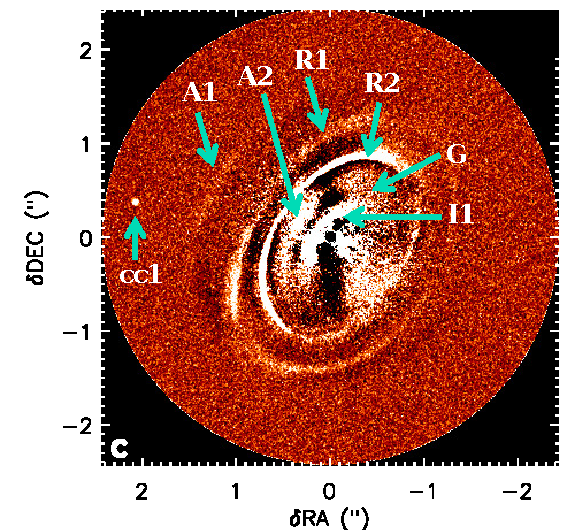
\includegraphics[width = 0.5\textwidth]{irdisjos}
\caption{Reduction of IRDIS ADI data. From the outside in, companion candidate (cc1), arc (A1), two full rings (R1 and R2), another arc (A2), a gap (G), and an innermost disk structure (I1). Figure adapted from \citep{DeBoer2016}}
\label{fig:irdisjos}
\vspace{-7mm}
\end{wrapfigure}

\noindent
two arcs (A1 and A2). A2 is confirmed to be a full ring, but the detections have not been deep enough to determine the origin of A1, it could either be a seperate ring or the backward facing side of R1 \citep{DeBoer2016}. In the rest of the document the abbreviations as introduced in Figure \ref{fig:irdisjos} will be used to indicate which part of the disk signal is being discussed.
\bigskip

A reduction of IFS T-LOCI ADI data, taken in the Y-J range, is available of the same dataset, which is illustrated in Figure \ref{fig:ifsjos}. T-LOCI (Template Locally Optimized Combination of Images \citep{Marois2010}) is an advanced way of selecting regions to make a reference to subtract the point spread function of the star from the data, but conserving the signal of the disk in the data. In this data one ring (R2), the inner disk component (I1) and the arc closest to the star (A2) are detected. The disk appears red in this image, but this could be an effect of the adaptive optics that performs better at longer wavelengths. No systematic analysis of the effects of different reduction methods have been done. It would be interesting to see if there are differences in performance between a classical ADI reduction and the T-LOCI reduction.

\begin{figure}[ht]
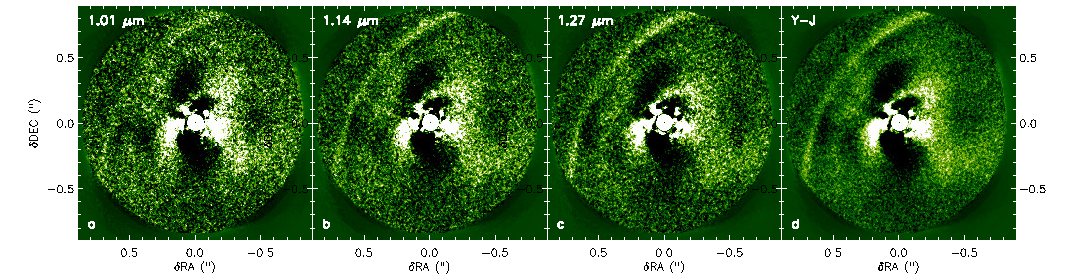
\includegraphics[width = \textwidth]{ifsjos}
\caption{Reduction of IFS ADI data. From left to right: \textbf{a:} median of the first 13 channels (0.96-1.07$\mu m$) \textbf{b:} median of 13 channels (1.08-1.21 $\mu m$) \textbf{c:} median of 13 channels (1.22-1.33 $\mu m$) \textbf{d:} median of the entire YJ range. Figure adapted from \citep{DeBoer2016}}
\label{fig:ifsjos}
\end{figure}

RX J1615 is also resolved with the Submillimeter Array (SMA) at 880 $\mu m$ \citep{Andrews2011} and the  Atacama Large Millimeter/submillimeter Array (ALMA) in 690 GHz continuum data \citep{VanderMarel2015}. These infrared observations probe deeper regions in the disk, measuring the emission of the gas and dust of the disk itself, mainly coming from the core or mid-plane of the disk where the pressure of the gas and dust is relatively high. Both observations show an inner cavity up to 20-30 au, confirming that RX J1615 hosts a transition disk. 
\bigskip

The spectral energy distribution (SED) of the star as determined by different research groups is illustrated in Figure \ref{fig:SED}. This figure displayes the contribution in flux of the object over the whole spectrum. The flux of the protostar is responsible for the contribution on the lower end of the SED. This contribution looks like a blackbody spectrum with a temperature of about 1900K, peaking around the H-band \citep{Padgett2008}. The slowly decreasing part on the high end of the SED is signal of the disk. The disk is mostly radiating in the infrared, due to its much lower temperature.

\begin{figure}[htb]
\centering
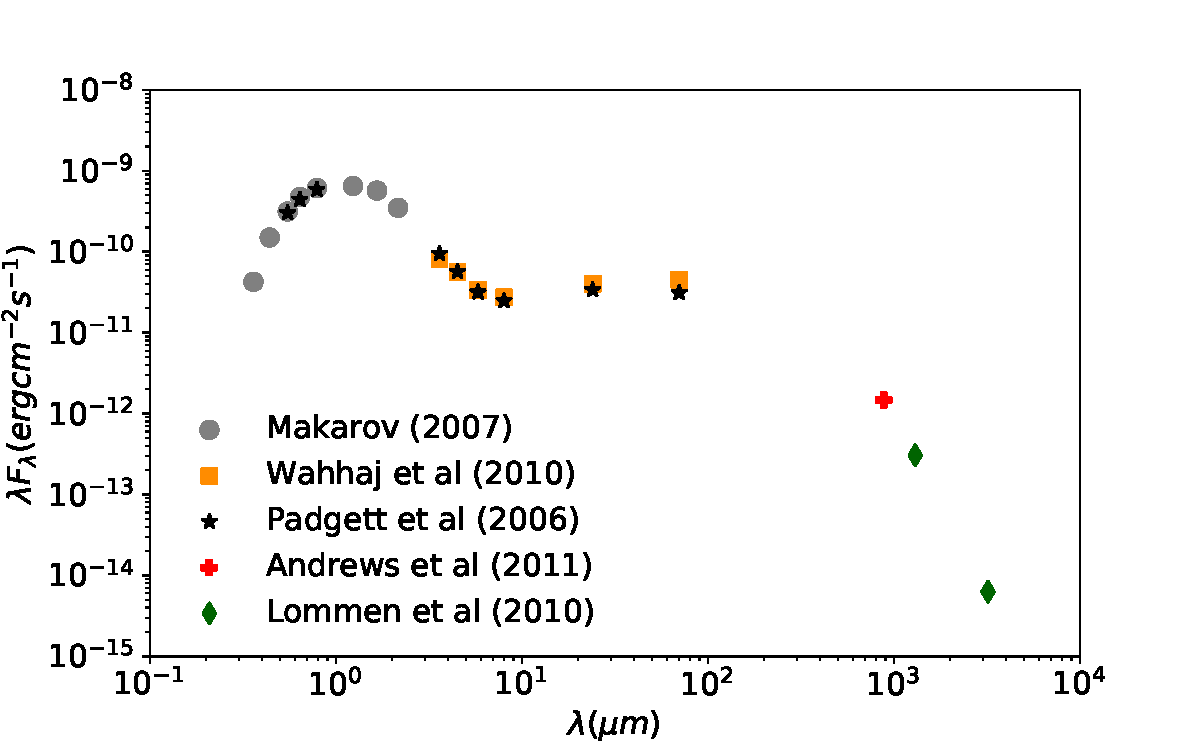
\includegraphics[width = \textwidth]{SEDnew.pdf}
\caption{The spectral energy distribution of RX J1615. The contribution on the left is due to stellar flux, the contribution at longer wavelengths is due to flux of surrounding structures \cite{Makarov2007}\cite{Wahhaj2010}\citep{Padgett2008}\citep{Andrews2011}\citep{Lommen2010}.}
\label{fig:SED}
\end{figure}

\chapter{Instrumentation}
\section{SPHERE}
\begin{figure}[hb]
\centering
\begin{subfigure}{.58\textwidth}
  \centering
  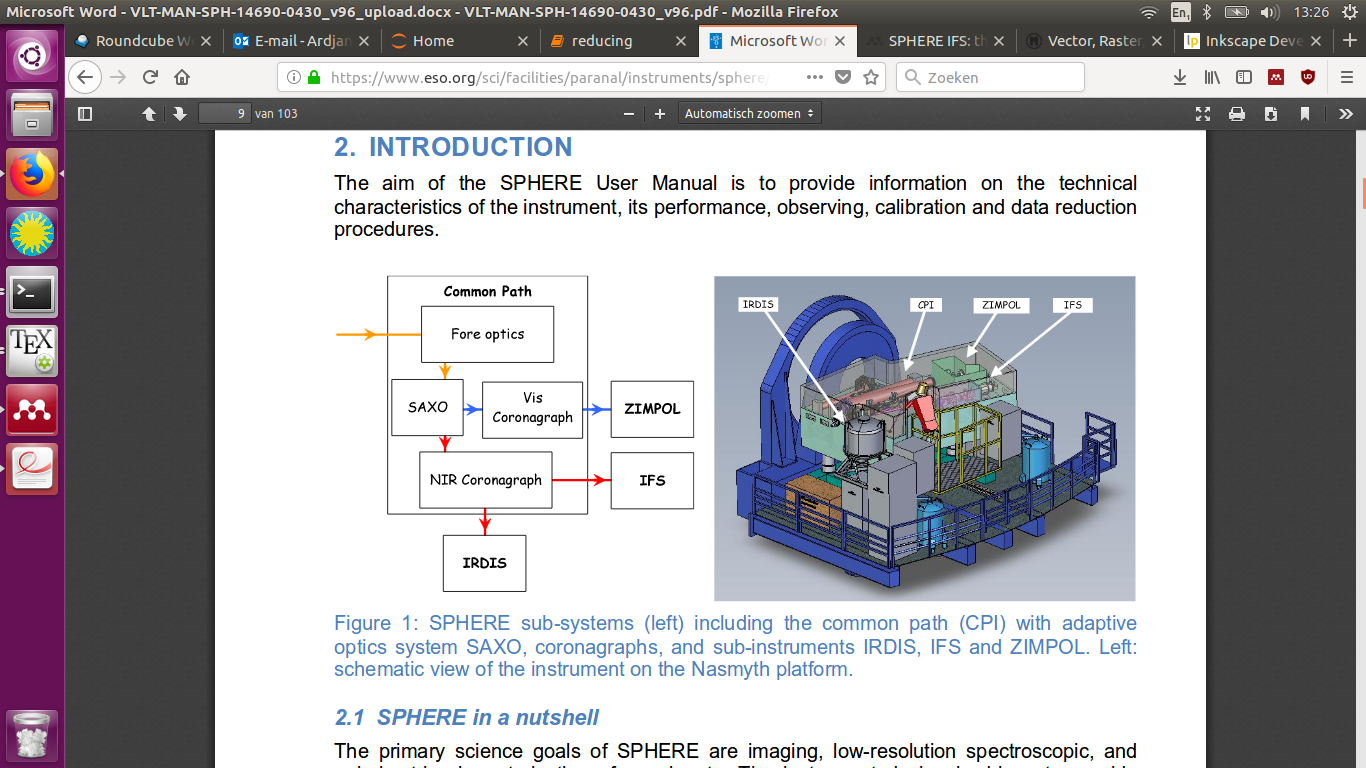
\includegraphics[trim={25cm 6cm 7cm 8.8cm},clip,width = 1\linewidth]{overviewSPHERE}
  \caption{Figure adapted from \citep{Observatory2007}}
  %\label{fig:sub1}
\end{subfigure}\hfill
\begin{subfigure}{.38\textwidth}
  \centering
  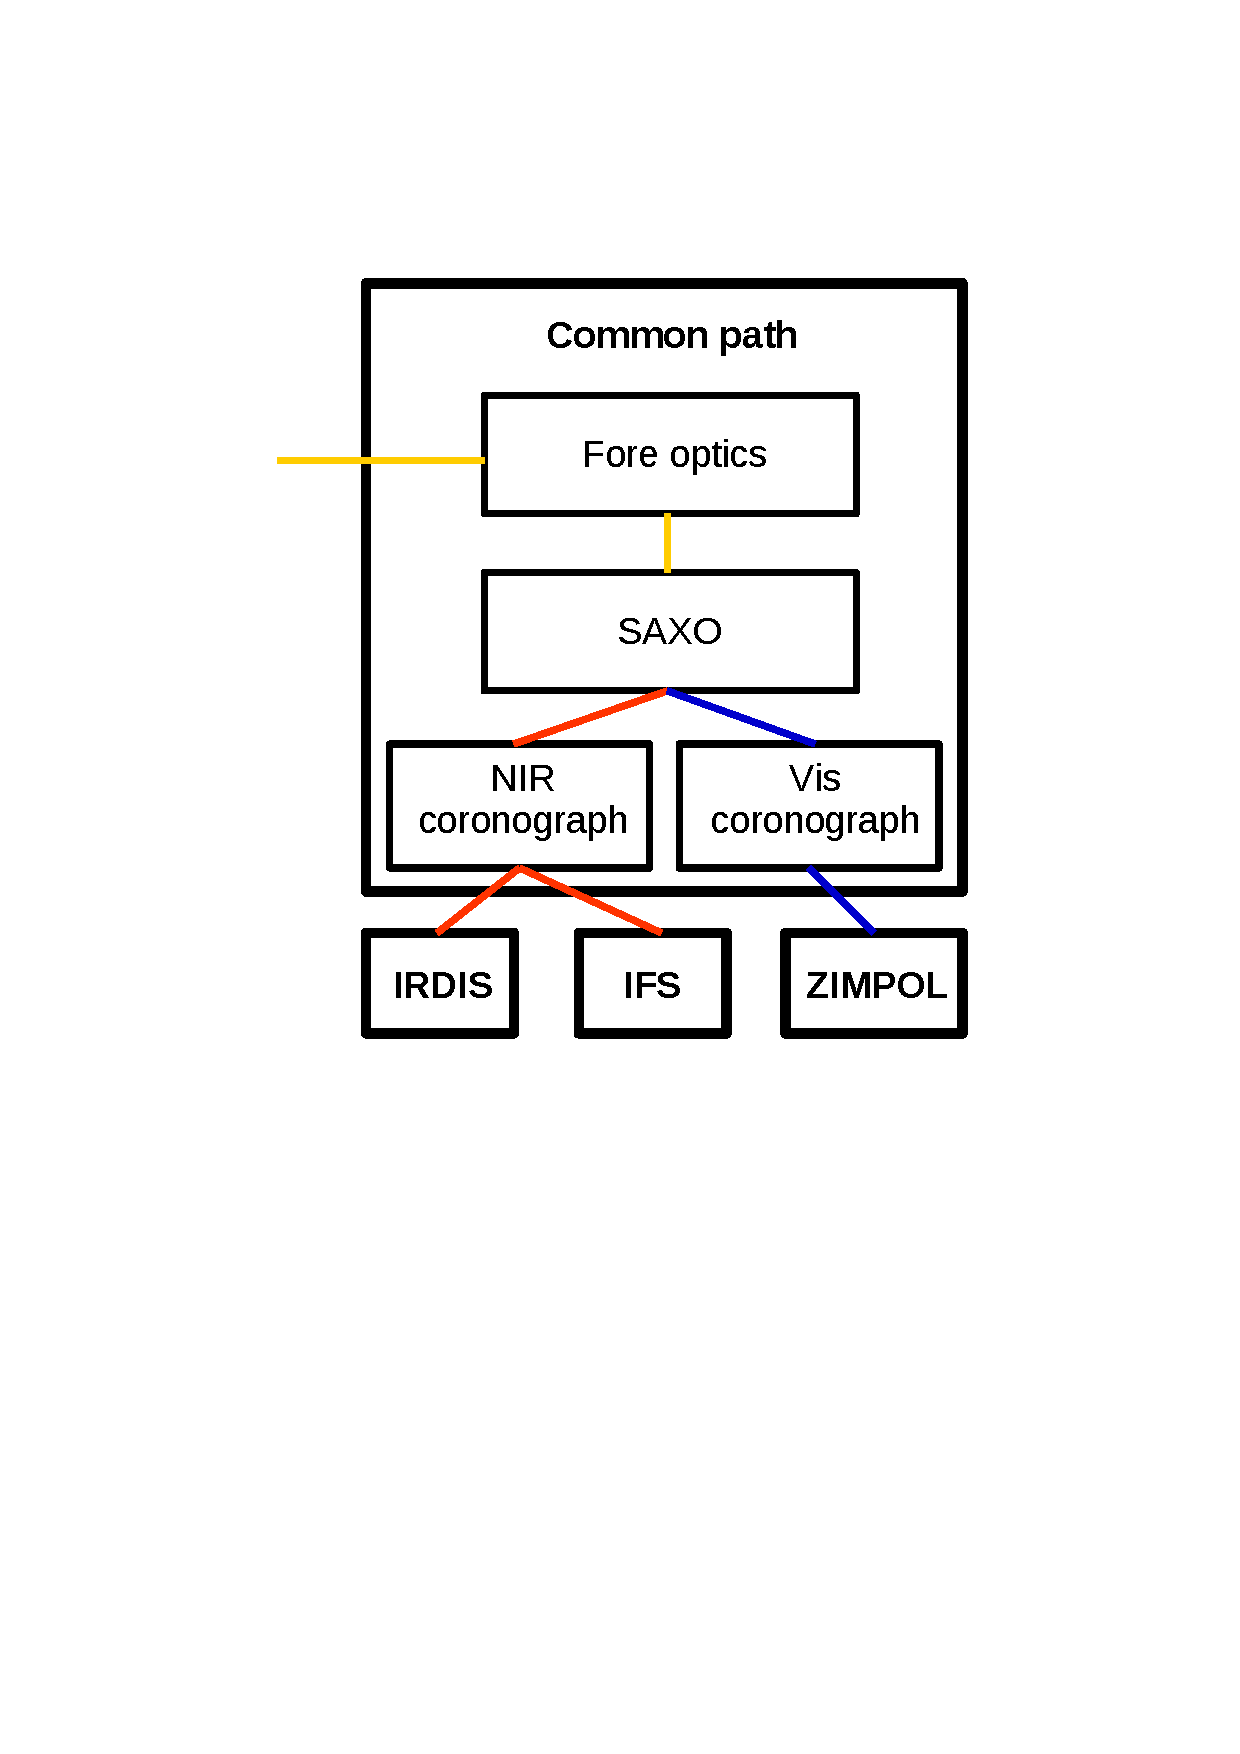
\includegraphics[trim={5cm 12cm 3.5cm 3.5cm},clip,width=1\linewidth]{overview_SPHERE}
  \caption{}
  %\label{fig:sub2}
\end{subfigure}
\caption{overview of SPHERE}
\label{fig:overviewSPHERE}
\end{figure}

SPHERE is an instrument for the VLT which is optimized for high contrast imaging. The instrument is placed in the Nasmyth of Unit Telescope 3 (UT3), one of the main VLT units, as illustrated in Figure \ref{fig:overviewSPHERE}. The instrument can be split up into four systems, the common path optics and the three subsystems: IRDIS, IFS and ZIMPOL. ZIMPOL (Zurich Imaging POL arimeter \cite{Thalmann2008}) uses visible light and IRDIS and IFS both near infrared light (NIR). Since IRDIS and IFS can work in parallel by use of a dichroic beamsplitter, we will discuss IRDIS briefly and take some time to look at the IFS in detail.

\subsection{Common path}
The common path (CPI) is the main system of SPHERE that powers all the cryostats and motors, corrects the light for many distortions and connects all the sub-systems to the light path. SAXO (Sphere Adaptive optics for eXoplanet Observation \citep{Sauvage2010}) plays an important role in the correction of the incoming light in CPI. Part of CPI are the coronagraphs that can be included in the light path to improve the contrast between the central star and surrounding structures.

\subsubsection{pupil stabilizing fore optics}
SPHERE has a derotater that is able to stabilize the field and the pupil on the detector. This stabilization is needed because of the rotation of the earth around its axis. The rotation of the earth causes a rotation of the field due to a change in parallactic angle and altitude of the object and a rotation of the telescope pupil with respect to the instrument due to the change in altitude of the object that is observed. In pupil stabilized mode, the field rotation is directly proportional to the change in parallactic angle of the object over time. The pupil has an offset with respect to the true north of -135.99$^o$, which means that all the data taken with SPHERE has to be rotated with that angle in order to make sure that north is pointing up. The field of view of the IFS is for technical reasons rotated with respect to the IRDIS field of view by 100.48$\pm$0.10 $^o$. The data in our dataset has hence to be rotated with a total offset of -35.51$^o$ in order to make sure that north is pointing up\cite{Maire2016}.
\bigskip

After entering the instrument, the light path is protected against many possible noise sources. The vibrations in the Nasmyth platform that are caused by seismic activity or other reasons are damped by use of servo-controlled pods and the whole instrument is protected against changes in temperature and dust by a protective cover. The light is then propagated in the complete spectral range from 0.450 $\mu m$ to 2.320 $\mu m$ to the first dichroic beamsplitter that splits the light. The visible part of the spectrum is used for ZIMPOL, the near infrared (NIR) part of the spectrum for both IRDIS and IFS. If ZIMPOL is not used, all visible light goes to the wavefront sensor that is used by SAXO to correct for the aberrations of the light in the atmosphere. After the first dichroic beamsplitter, the light is guided through an atmospheric dispersion corrector (ADC) that corrects for dispersion effects in the atmosphere that are caused by the change in altitude of the object over time.
\bigskip

\subsubsection{adaptive optics}
SAXO is the adaptive optics module of SPHERE. It is composed of different components, each correcting a part of the distortion of the light. The bundled information of these components is sent to the deformable mirror (DM), that corrects for phase perturbations of up to a frequency of 1.2 kHz by use of the 41x41 actuators that deform the mirror \citep{Hugot2012}. The phase perturbations are measured by different components.
\bigskip

\begin{figure}[htbp]
\centering
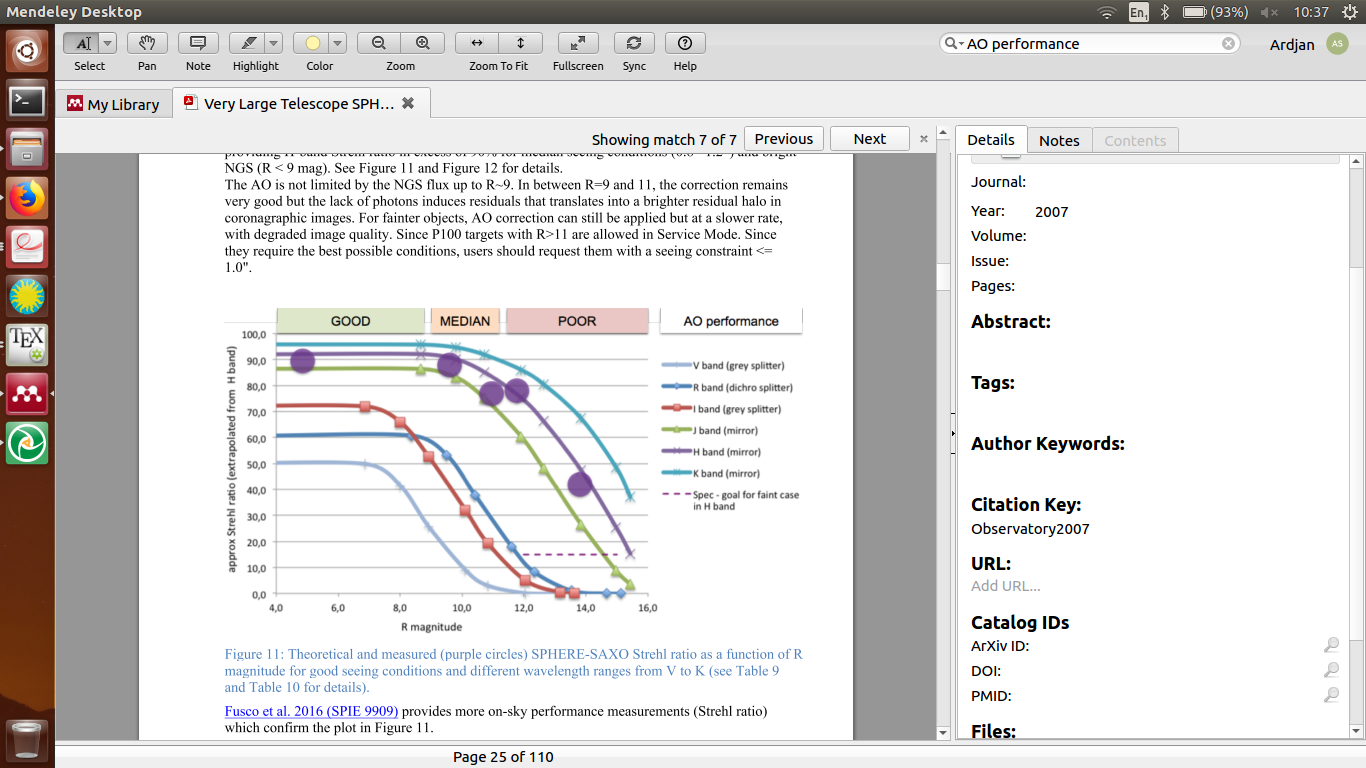
\includegraphics[trim={7cm 4.5cm 19cm 10cm},clip,width = 1\textwidth]{aoperformance}
\caption{Theoretical and measured (purple circles) SPHERE-SAXO Strehl ratio as a function of R magnitude for good seeing conditions and different wavelength ranges from V to K. Figure adapted from \citep{Fusco2014}}
\label{fig:aoperformance}
\end{figure}

The turbulence is measured by a wavefront sensor that transposes the phase shift to an intensity distribution on a detector. The wavefront sensor that is used is a Shack-Hartmann sensor \citep{Anugu2013}. This sensor uses a 40x40 lenslet array that produces a spot for each lenslet on a detector that has 240x240 pixels. A distorted incoming wavefront changes the position of the focal spot of the lenslets on the sensor, which can be used to calculate the local tilt of the wavefront. Other distortions such as image motion and pupil shift are measured with tip tilt sensors, correcting only the large scale variations that these distortions cause.
\bigskip

\begin{figure}[!b]
\centering
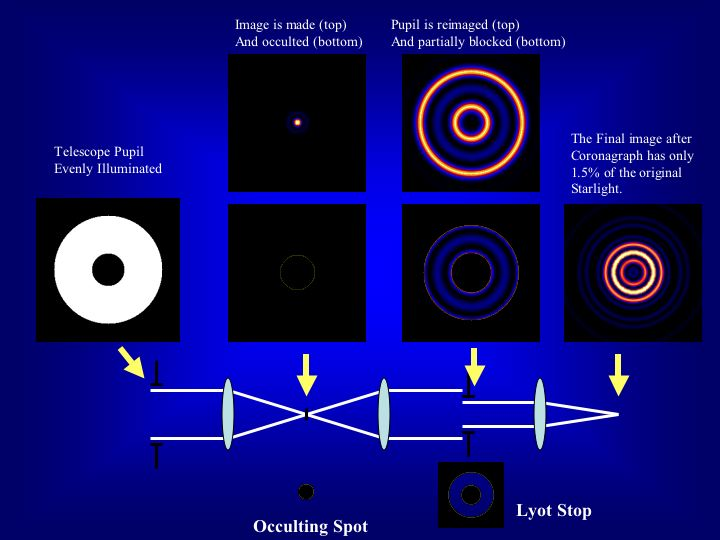
\includegraphics[trim={0cm 0cm 0cm 0.3cm},clip,width = 0.85\textwidth]{coronagraph}
\caption{Explanation of the working of a Lyot coronagraph. Figure adapted from \citep{Sivaramakrishnan2001}}
\label{fig:coronagraph}
\end{figure}

The incoming wavefront of the object is accurately corrected in a radius of about 20 $\lambda/D$ in the image plane. Further out, the PSF is still corrected, but not enough to suppress the stellar halo. The correction of the AO is dependent on the magnitude in the R-band (618nm-674nm \citep{Mouillet2013}), since the Shack-Hartmann sensor measures the perturbations of the wavefront in the range of the R filter. The more light is provided to the sensor, the more accurately the distortions of the wavefront can be measured, which drastically changes the overall performance of the AO system and hence the quality of the data. The performance of the AO as a function of R magnitude is illustrated in Figure \ref{fig:aoperformance}, where the performance is expressed in terms of Strehl ratio. Strehl ratio is roughly defined as the ratio between the peak of the measured PSF divided by the peak of an ideal PSF.

\subsubsection{coronagraphs}
A coronagraph is a device that increases the contrast between the star in the center and the background. SPHERE has several coronagraphs for different conditions the instrument can work in. All coronagraphs consist of three components. At the beginning of the light path an apodizer changes the beam profile and thus improves the dynamic range of the image. Further downstream in the focus of the secondary mirror, a focal plane mask absorbs most of the light from the center of the beam, which means that after reimaging the excess light of the center is concentrated around the edged of the telescope pupil. This excess light is absorbed by a lyot stop that blocks most of the light on the edges of the beam, but allows light from surrounding sources to pass. Different combinations of these three elements have different results on the final image and for all conditions there is a combination that works, think of the wavelength range that is used at that moment, seeing and needed inner working angle. An elaborate explanation of the working of the coronagraphs in SPHERE is illustrated in Figure \ref{fig:coronagraph}.

\subsection{IRDIS}
\begin{figure}[!b]
\centering
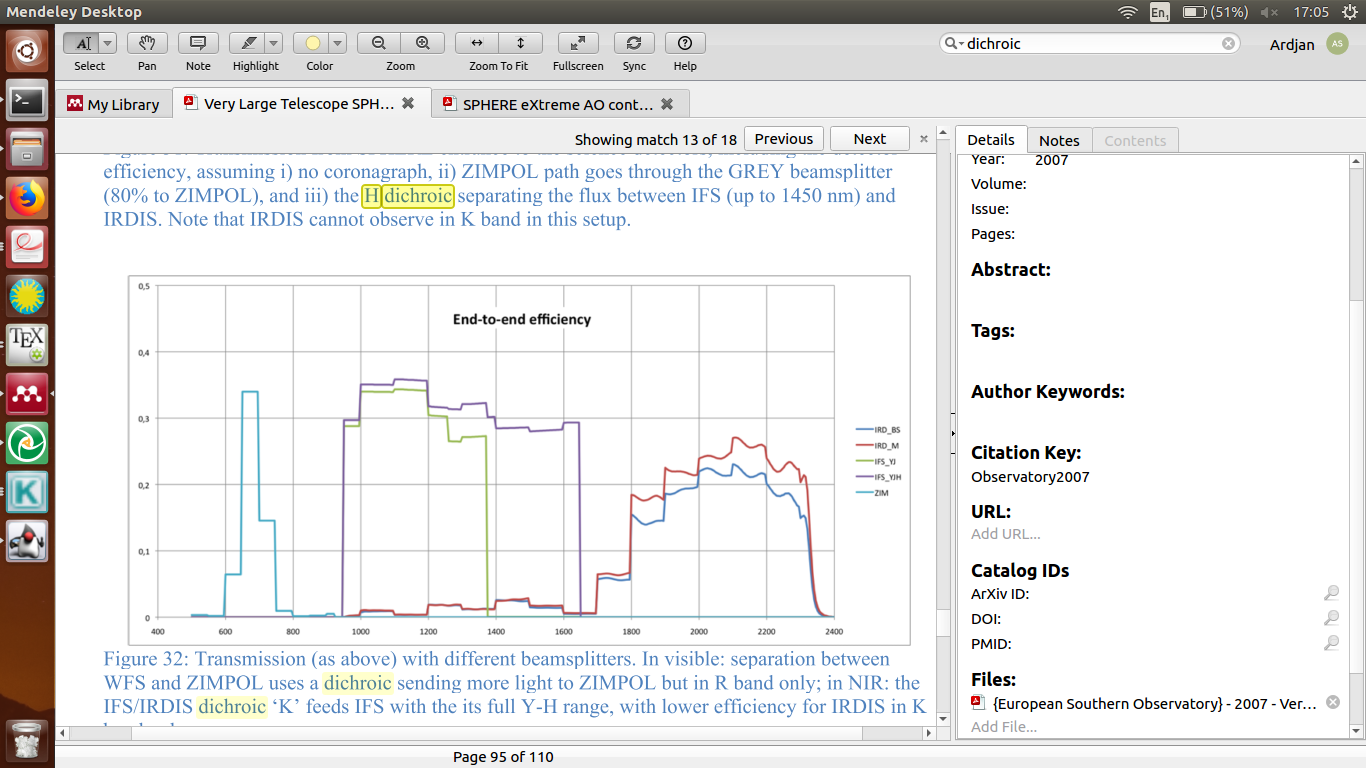
\includegraphics[trim={4cm 4.3cm 16cm 9cm},clip,width = \textwidth]{systemthroughput}
\caption{End-to-end efficiency if both IFS and IRDIS get light in parallel mode. The light of ZIMPOL is in this case for the AO system. Note that only the IRDIS curves are shown in case the instrument is set up in IRDIFS\_EXT mode. Figure adapted from \cite{Observatory2007}}
\label{fig:systemthrougput}
\end{figure}

IRDIS has a field of view of 11"x12.5" and has several modes in which data can be acquired. The NIR part of the beam that is seperated by the first dichroic beamsplitter can be used in two different way. All the light can be reflected on a mirror to IRDIS, which provides classical imaging, dual band imaging, dual-polarization imaging with the filters Y to Ks and long slit spectroscopy. Another possibility is to use a second dichroic beamsplitter that allows to use both IRDIS and IFS for longer and shorter wavelengths respectively. Two different dichroic beamsplitters are possible in this case. If the instrument is set up in IRDIFS mode, the IFS receives light in the Y-J band and IRDIS is able to do narrow band or broad-band H dual band imaging in parallel. In IRDIFS\_EXT mode, the IFS receives light in the range from the Y band to H band, leaving IRDIS with the possibility to get dual band imaging data with lower efficiency in a narrow-band filter or in broad-band K. The end-to-end efficiencies of both possibilities are shown in Figure \ref{fig:systemthrougput}. 

\section{Integral Field spectrograph}
\begin{figure}[hb]
\centering
\begin{subfigure}{.65\textwidth}
\centering 
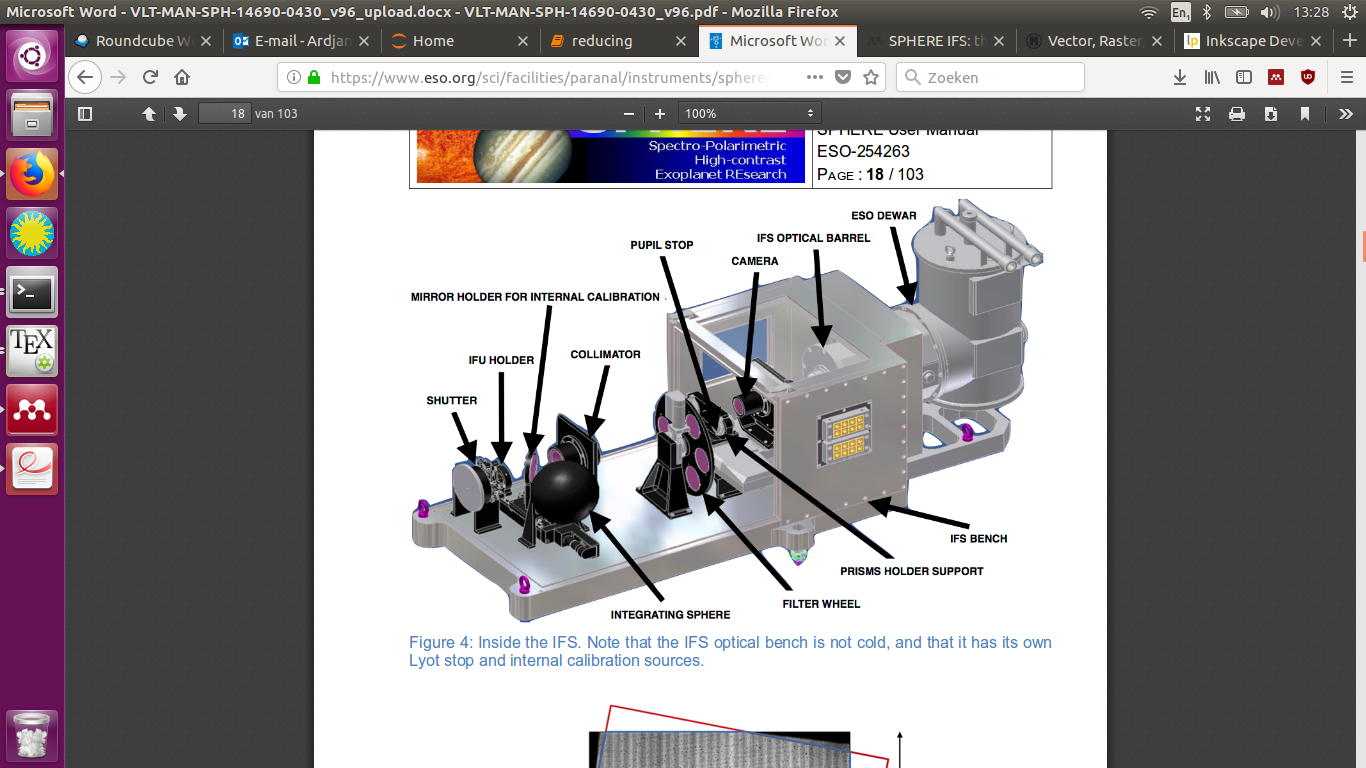
\includegraphics[trim={12cm 5cm 12cm 7cm},clip,width = 1\linewidth]{overviewIFS}
\caption{Figure adapted from \cite{Observatory2007}} 
%\label{overviewIFS}
\end{subfigure}\hfill
\begin{subfigure}{.30\textwidth}
  \centering
  %\begin{turn}{270}
  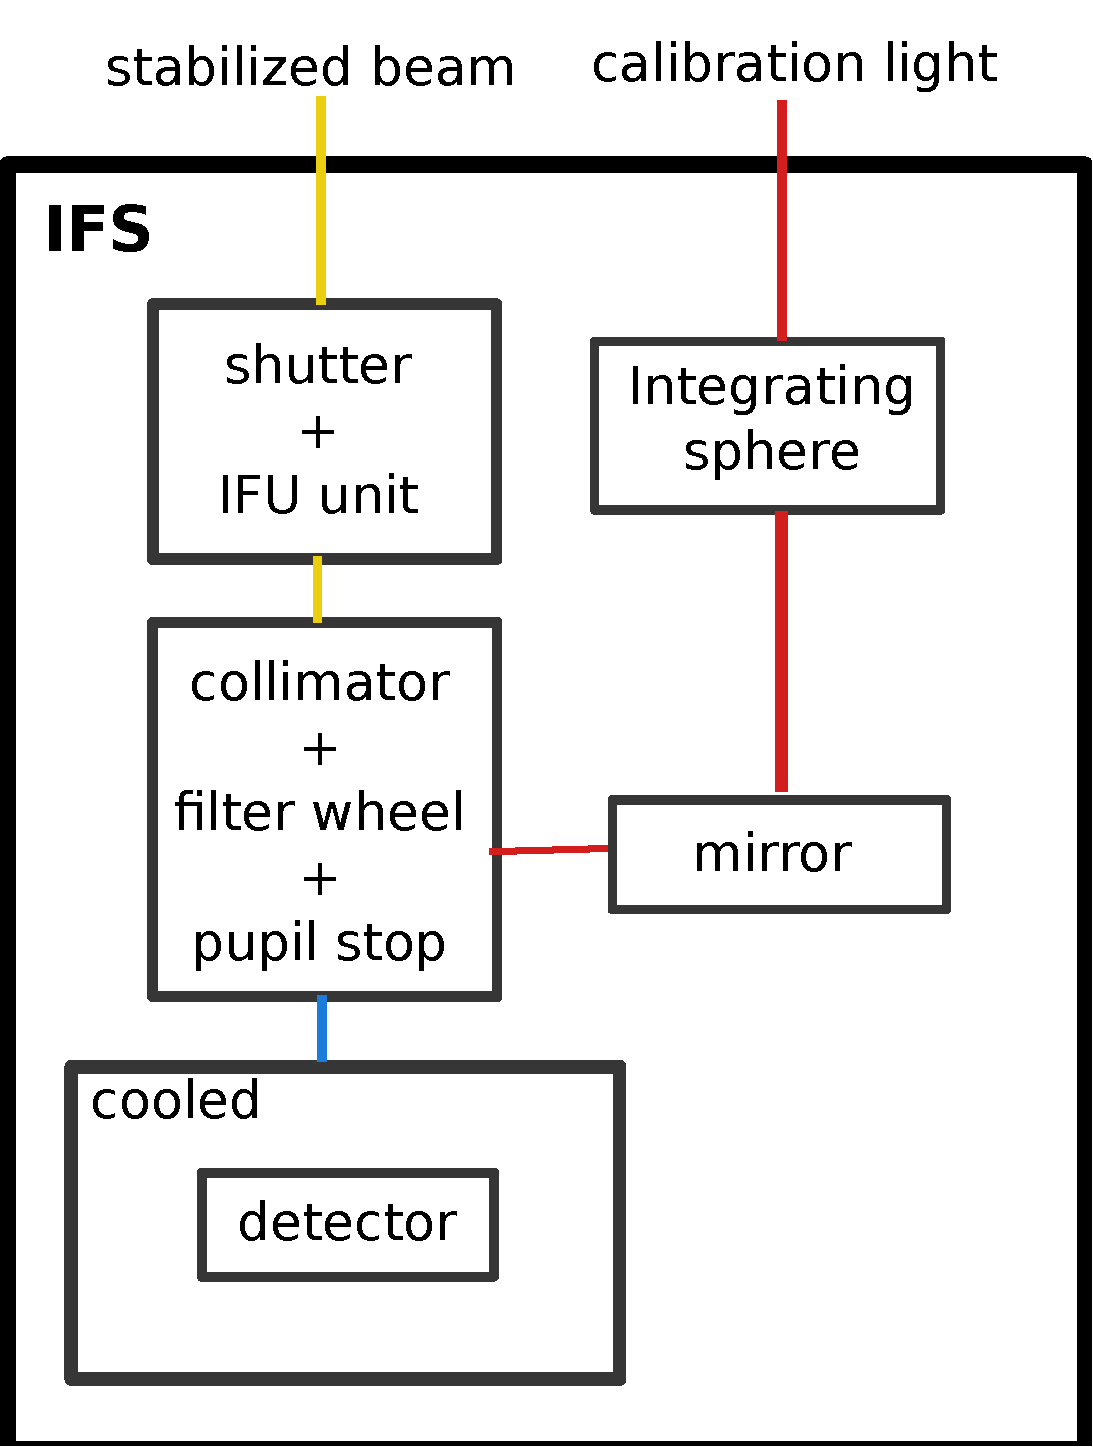
\includegraphics[trim={0cm 0cm 0cm 0cm},clip,width=1\linewidth]{overview}
  %\end{turn}
  \caption{}
  %\label{fig:sub2}
\end{subfigure}
\caption{overview of SPHERE/IFS}
\label{fig:overviewIFS}
\end{figure}

The integral field spectrograph is a subsystem of SPHERE that is able to collect data over a wavelength range from 0.95 $\mu m$ up to 1.346 $\mu m$ or 1.677 $\mu m$,  depending on the NIR dichroic beam splitter (Y-J or Y-H) that is used. The spectral resolution of the IFS is on average R = 55.1 in Y-J mode and R = 34.5 in Y-H mode. The IFS has a total field of view of 1.73"x1.73", which is much smaller than IRDIS's, but enough to be able to detect structures of protoplanetary disks close to the star.
\clearpage 

\subsection{IFU unit}
\begin{wrapfigure}{R}{0.5\textwidth}
\centering 
\vspace{-9mm}
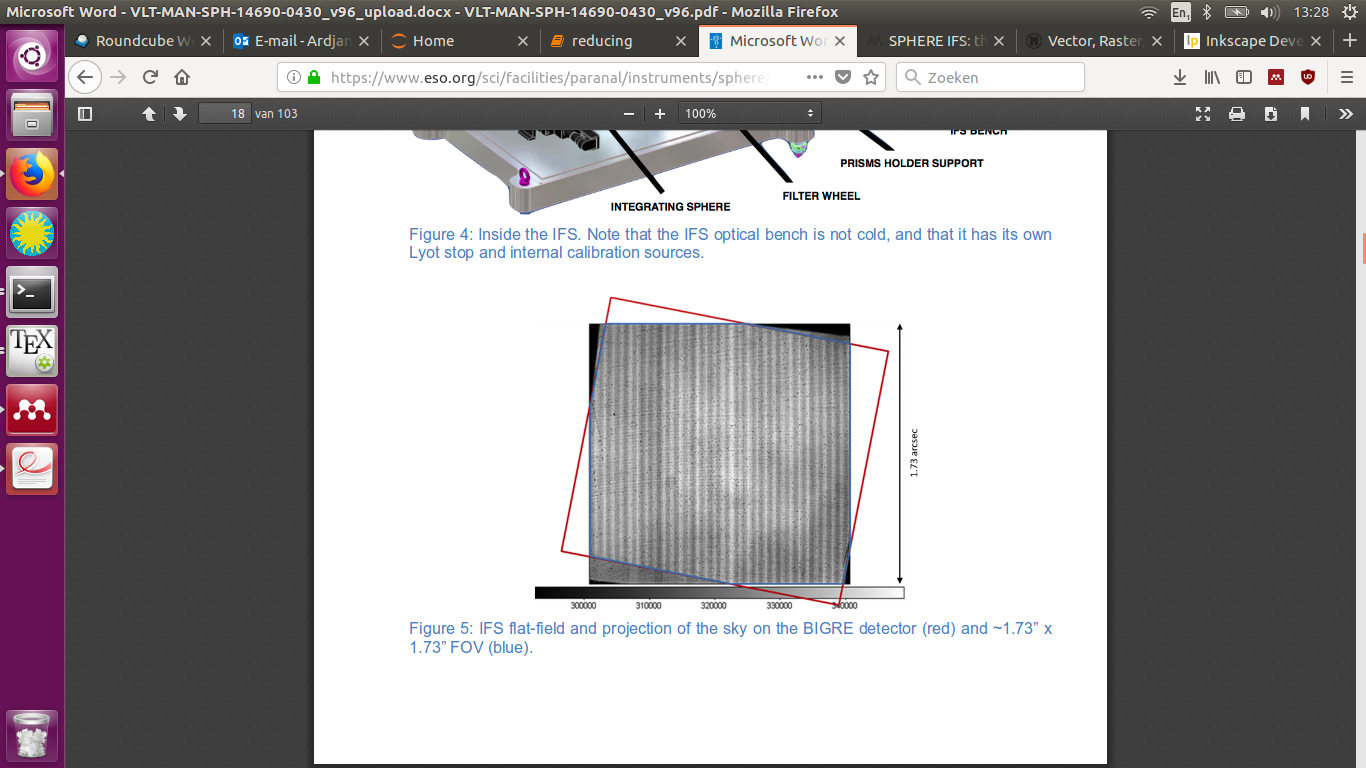
\includegraphics[trim={19cm 5.5cm 14cm 10cm},clip,width = 0.9\linewidth]{biggre}
\caption{IFS flat-field and projection of the sky. In red the arrangement on the BIGRE detector and in blue the useful FOV. Figure adapted from \citep{Observatory2007}}
\label{fig:bigre}
\vspace{-7mm}
\end{wrapfigure}

The IFS is able to obtain spectral information by use of BIGRE \cite{Antichi2009}, an integral field unit consisting of 122x122 microlenslets with a diameter of 150 $\mu m$, in a hexagonal grid, as illustrated in Figure \ref{fig:bigregrid}. This grid is rotated by $10.7^o$ with respect to the dispersion in order to get the most lenslets stacked on the grid. This results in a small section of the detector to be meaningless, as illustrated in Figure \ref{fig:bigre}. The FWHM of these spectra is at the middle of the spectral range 29.6 mas. The spatial sample scale of the detector is 12.3 mas, which increases the angular resolution, and has still a good enough signal to noise ratio (SNR) on the detector. The spectra of these lenslets are projected on the detector in a rectangular area with dimensions 5.1x41 pixels \citep{Claudi2006}.
%\vspace{0.5cm}

\subsection{Detector}
\begin{figure}[!b]
\centering 
\vspace{-0.5cm}
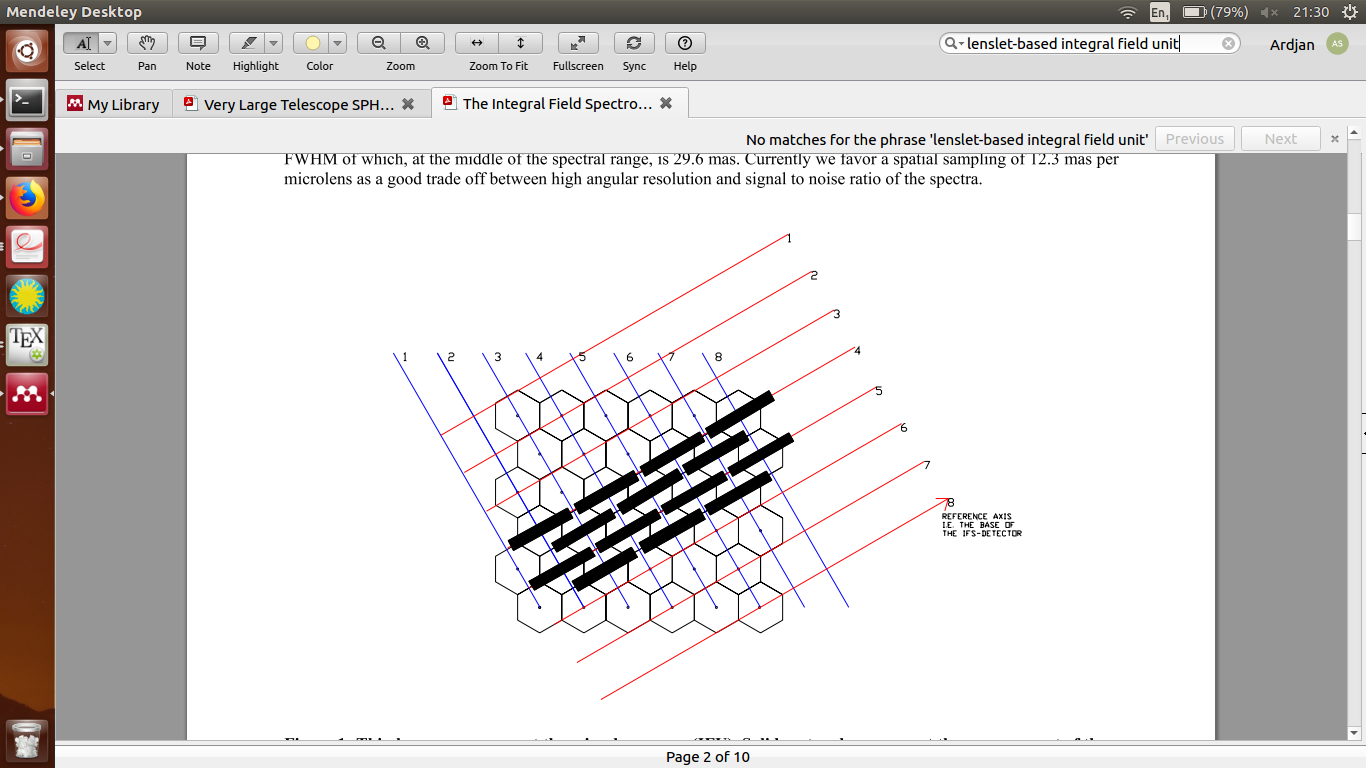
\includegraphics[trim={13cm 1.7cm 10cm 8cm},clip,width = 0.65\linewidth]{bigregrid}
\caption{The hexagonal lines represent the different microlenses of the IFU, the solid rectangles represent the spectra of the lenslets on the detector, the numbered lines  represent the orientation of the IFS Detector. Figure adapted from \cite{Claudi2006}} 
\label{fig:bigregrid}
\vspace{-0.5cm}
\end{figure}

The detector of the IFS is 2048x2048 pixels big, each pixel corresponding to (7.46 mas)$^2$. The incoming light of the IFS is filtered by an additional filter that has a sharp cut-off at the desired wavelength, which allows the detector to be a standard infrared detector. It is technically possible to block longer wavelengths by use of the cut-off wavelength at which an HgCdTe detector is no longer sensitive, but this would make the instrument unnecassary complex and would increase the readout noise drastically from ~10 $e^-$ to ~25 $e^-$ \citep{Claudi2006}. This cut-off allows cooling only the detector, keeping the optics at room temperature. The contribution of the thermal background to the noise is nigligible since all radiation at wavelengths longer than 1.35 $\mu m$ is blocked. The detector is cooled with liquid Nitrogen, which reduces the thermal noise of the detector\citep{Claudi2006}. The detector is static and does not need to be rotatable since the rotation of the field and the pupil are corrected in the derotator. 

\subsection{Calibration devices}
The IFS has two calibration arms to provide a proper calibration of the instrument. The first arm is mounted in the common path and consists of a few calibration lamps. These lamps can be used to measure the throughput of the lenslet grid and the different optical components of the IFS. Four additional lasers with wavelengths of respectively 0.9877, 1.1237, 1.3094 and 1.5451($\mu m$) are also provided on this calibration arm for the wavelength calibration. Each of the lasers is focused on a different part in the spectra on the detector by the IFU. Interpolation between these points gives an accurate model for the wavelength solution for each pixel, which can be used to reduce the data.
\bigskip

The second calibration arm is mounted internal to IFS, after the IFU, such that flats can be taken that measure the sensitivity of the whole detector. This is not possible with the external calibration lamps, since the detector has bigger dimensions than the FOV of the lenslet grid. Decoupling the noise of the IFU and the detector makes the calibration slightly better and this allows to take calibration frames in parallel with IRDIS taking calibration frames, making the calibration process for both subsystems much faster. The internal calibration arm consists of five calibration lamps: four narrowband lamps, centered around 1.0, 1.2, 1.3 and 1.5 $\mu m$, with a full width half maximum (FWHM) of about 0.01-0.04 $\mu m$ and one broadband white lamp\citep{Desidera2008}. An integrating sphere is also provided that spreads the light of the different lamps evenly over the whole detector. An elaborated description of the different calibration steps is given in the methodology chapter.

\chapter{Methodology}
\section{IFS reduction for dummies}
\begin{figure}[!b]
\centering
\begin{subfigure}{.48\textwidth}
  \centering
  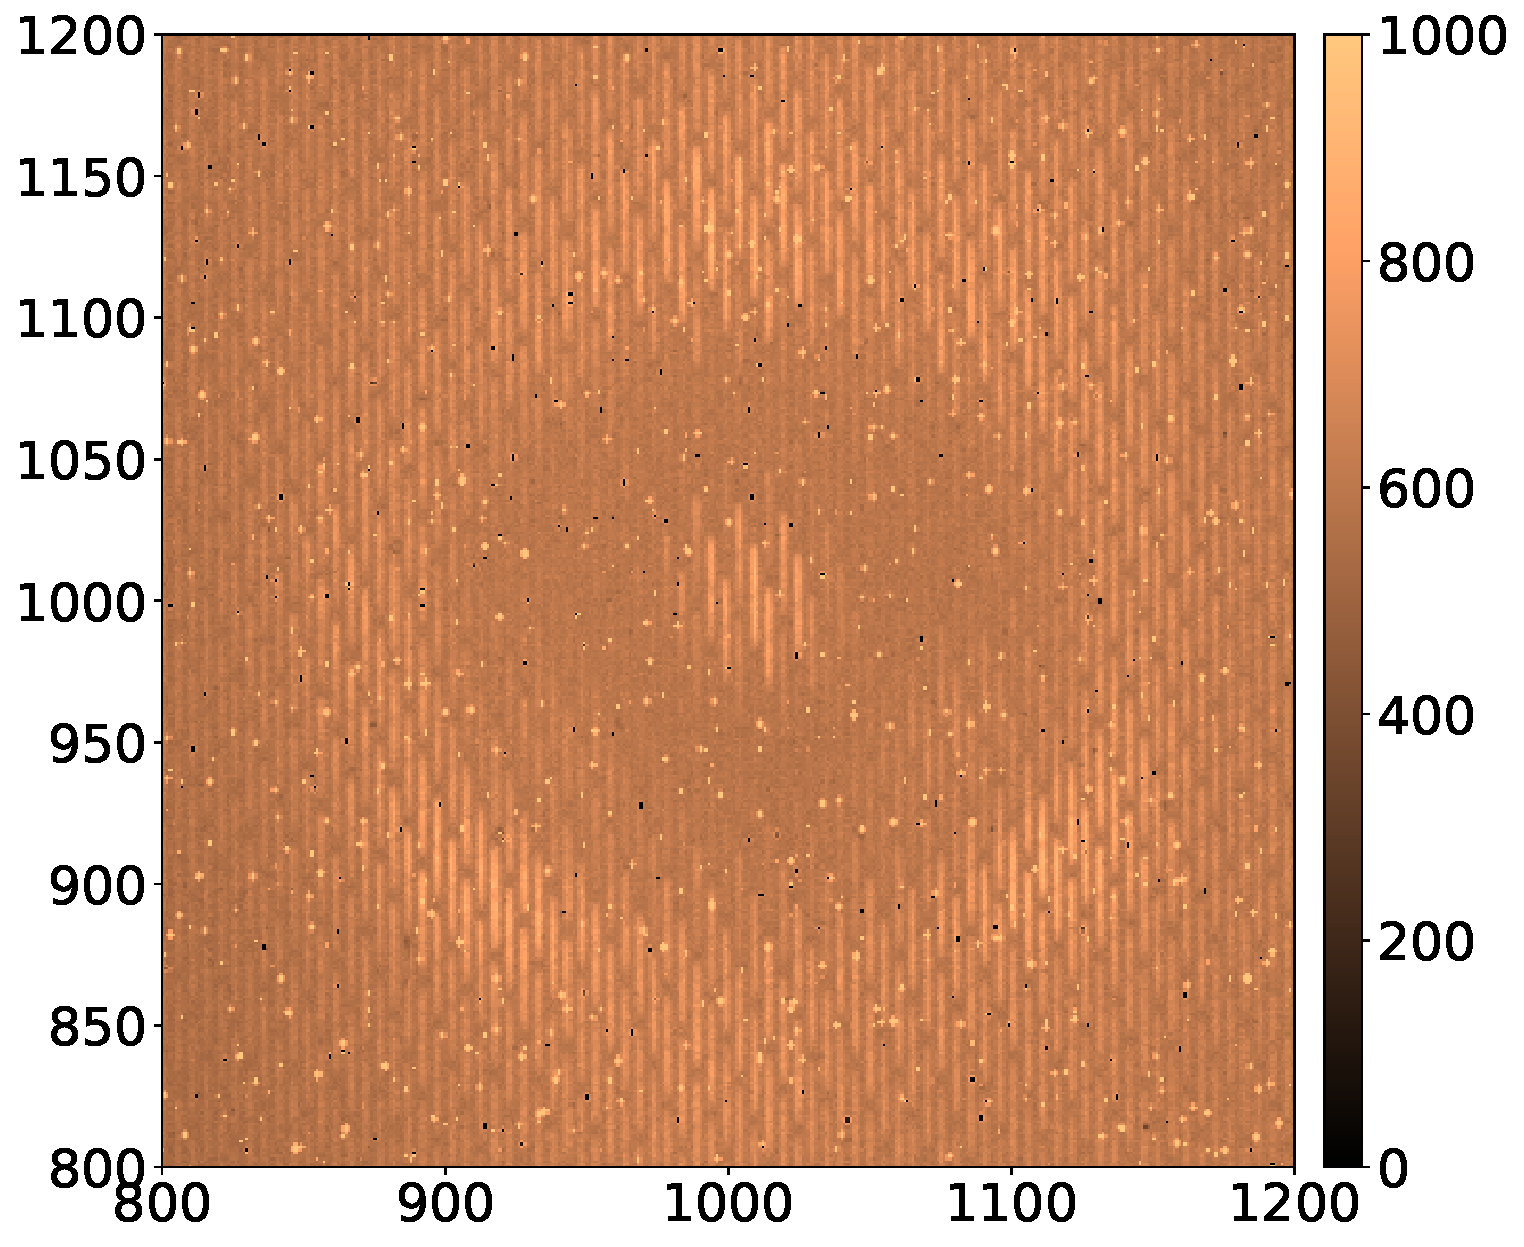
\includegraphics[width=1\linewidth]{rawframe}
  \caption{zoom of one of the raw science frames}
  \label{fig:rawdata}
\end{subfigure}\hfill
\begin{subfigure}{.48\textwidth}
  \centering
  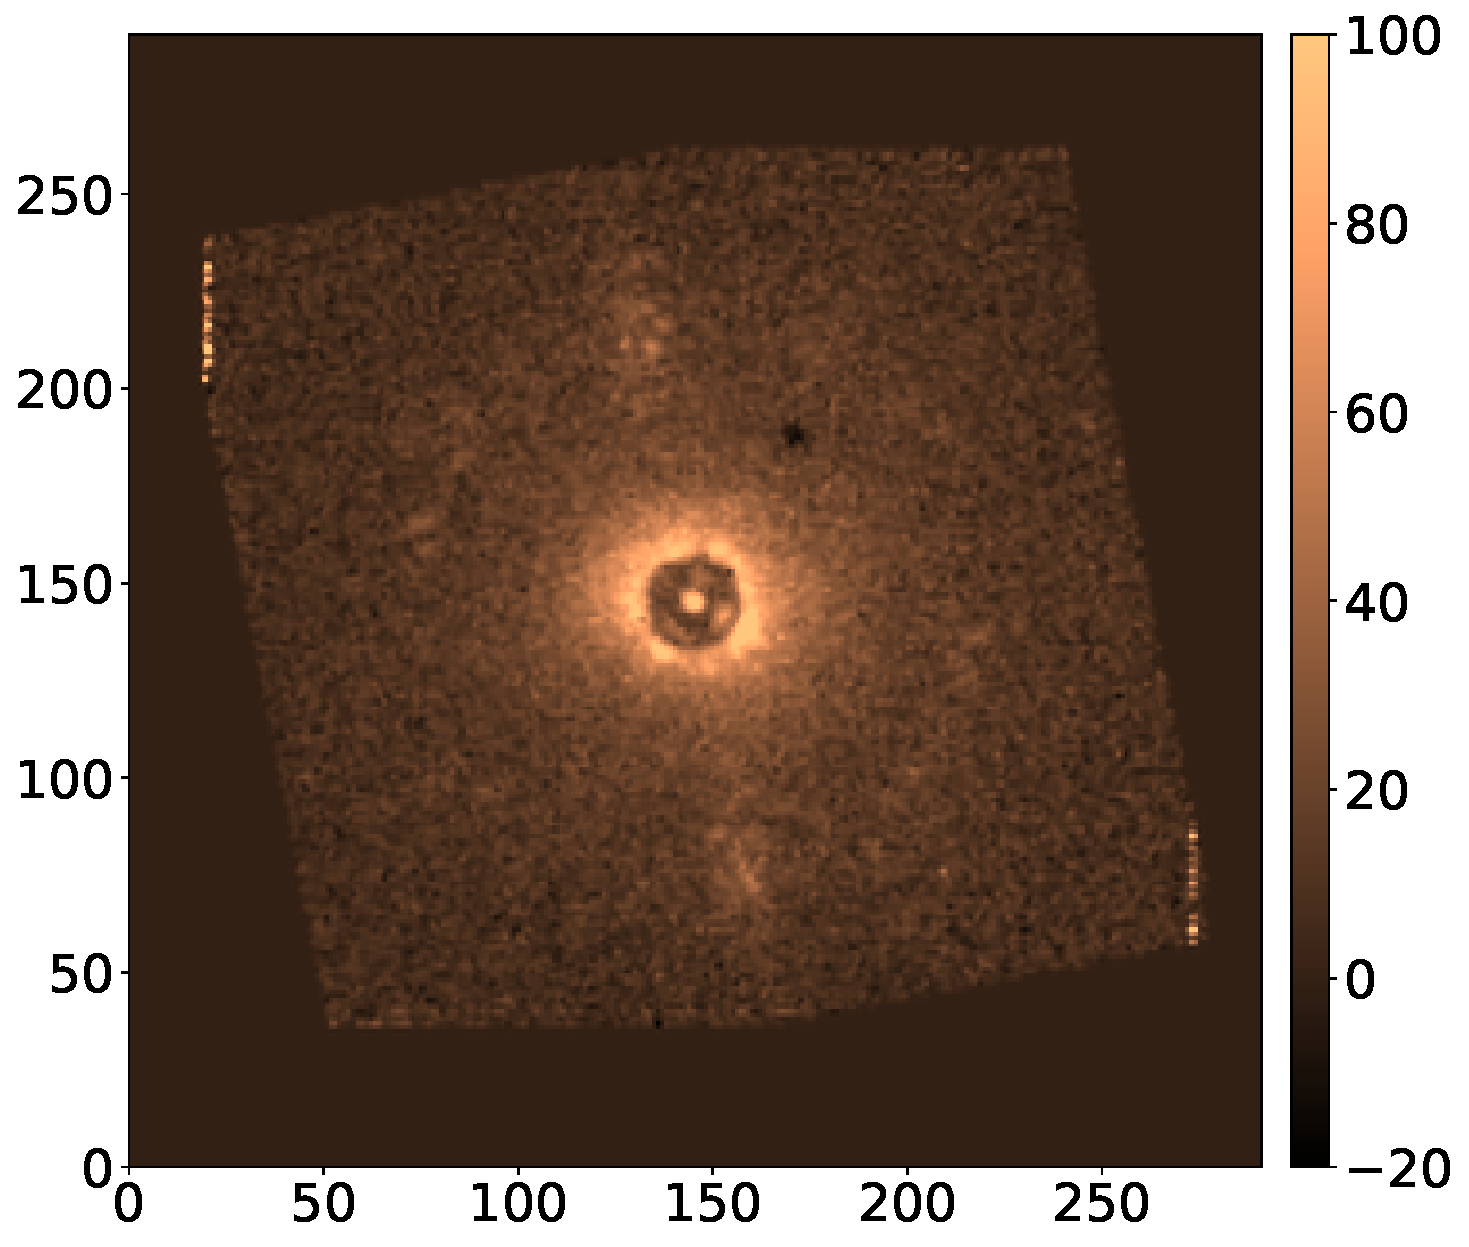
\includegraphics[width=1\linewidth]{reducedframe}
  %\hspace{7 mm}
  \caption{one of the 39 wavelength slices of a reduced science frame}
  \label{fig:reduceddata}
\end{subfigure}
\caption{the result of the basic reduction}
\label{fig:datareduction}
\end{figure}
Data taken with an integral field spectrograph contains a spectrum for each pixel, called a spaxel. A raw data file is illustrated in Figure \ref{fig:rawdata}. To reduce this to a cube with a frame for each spectral channel as illustrated in Figure \ref{fig:reduceddata}, several calibrations are needed. At first the dark current has to be subtracted and pixel-to-pixel sensitivity of the detector has to be normalized using detector flat frames. After that the different spectra have to be located and the wavelength of all pixels calibrated, whereafter the science reduction produces the resulting datacube that consists of 39 spectral channels, each with a dimension of 291x291 pixels.
\bigskip

The Common Pipeline Library (CPL)\citep{Observatory2007} is a library of commands that is able to do the basic reduction steps of SPHERE data. Running the CPL can be done by use of Esorex, which is a commandline driven package, or EsoReflex. Esorex requires the use of a set of frames (sof) file for each recipe. This can easily be automatized, but since it is much work to write a code that identifies the different calibration data and mistakes can easily be made in the selection of the required data, we used EsoReflex for the reduction, which provides an easy and flexible way to run the different recipes of the pipeline. EsoReflex provides a user interface in the form of a workflow with a setup of a basic reduction pipeline in advance, which can be adapted in an easy way. It identifies all the required data that is unsorted stored in the input directory and gives a warning if something is missing. The workchart of EsoReflex that is used to reduce the data is added as an appendix.
\bigskip

The data needed for a basic reduction is listed in table \ref{Tab:data}. Note that all the data has to be taken in the same mode as the science frames. All calibration data needs a corresponding dark frame with the same exposure time. The detector flats however are taken with many different exposure times. In order to deal with this, two detector flats are needed per calibration lamp with different exposure times. The flat with shortest exposure time acts in the reduction as a dark and bias frame for the other one. This is possible since the flats give relative values by which the pixels have to be divided to measure uniform light, which means that the values are also typically close to one. 
\bigskip

All individual reductions of calibration data have an own recipe in the common pipeline. A good understanding of these recipes and the corresponding calibration files is useful to get clean results in the end. The floatchart that summarizes the steps we took to reduce the data is appended together with the corresponding sof files.

\begin{longtable}{| p{.20\textwidth} | p{.12\textwidth} | p{.58\textwidth }|}
\hline
\textbf{data type} & \textbf{number} & \textbf{comments}\\\hline
science frames&  &can be multiple frames stacked together as a single file with .fits extension.\\\hline
spectral positions & 1 & exposure time of 1.6507260s$^*$	\\\hline	
wavelength calibration & 1 & exposure time of 1.6507260s$^*$ \\\hline
detector flat lamp 1 & 2 & two different exposure times\\\hline
detector flat lamp 2 & 2 & two different exposure times\\\hline
detector flat lamp 3 & 2 & two different exposure times\\\hline
detector flat lamp 4$^{**}$ & 2 & two different exposure times\\\hline
detector flat lamp 5 & 2 & two different exposure times\\\hline
instrument flat & 1 & \\\hline
background calibration & 1 & same exposure time as the science frames\\\hline
dark & & for all calibration frames one with corresponding exposure time\\\hline
\caption*{\\$^*$ shortest exposure time possible\\ $^{**}$ only if science data is taken in YH mode}\\% needs to go inside longtable environment
\caption{Data needed for the reduction of a science frame}%
\label{Tab:data}
\end{longtable}%

\subsection{Master dark}
The master dark recipe median combines multiple raw dark frames into one master dark. From the master dark, this recipe determines the position of pixels that give strange results in all measurements, which are called static bad pixels. It returns both a file that contains a master dark frame, consisting of the image, bad pixels, the rms and the weightmap and a file that contains a static bad pixel map, which has the same content as the second extension in the master dark frame. An example of a master dark image is illustrated in Figure \ref{fig:masterdark}. 
\bigskip

If a background calibration file is provided to the final science reduction, the background calibration file is used to correct for the dark current. The difference between these two is small. The only difference is that a normal dark is taken in N\_NS\_OPAQUE infrared IRDIS coronagraph combination mode and a background calibration in N\_NS\_CLEAR, meaning that the combination of coronagraphs used to take the data has changed\cite{Mouillet2013}.

\begin{figure}[!t]
\centering
\begin{subfigure}{.48\textwidth}
  \centering
  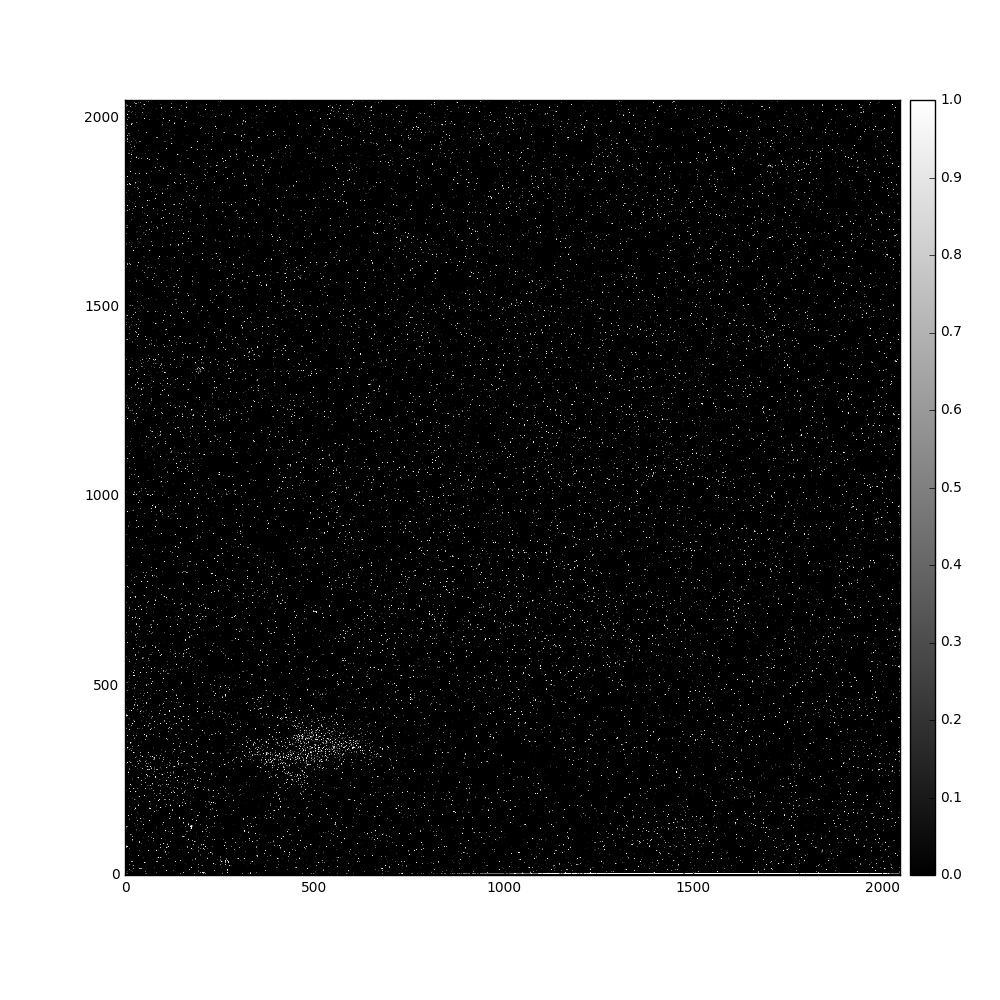
\includegraphics[width=1\linewidth]{badpixelmap}
  \caption{bad pixel map}
  %\label{fig:sub1}
\end{subfigure}\hfill
\begin{subfigure}{.48\textwidth}
  \centering
  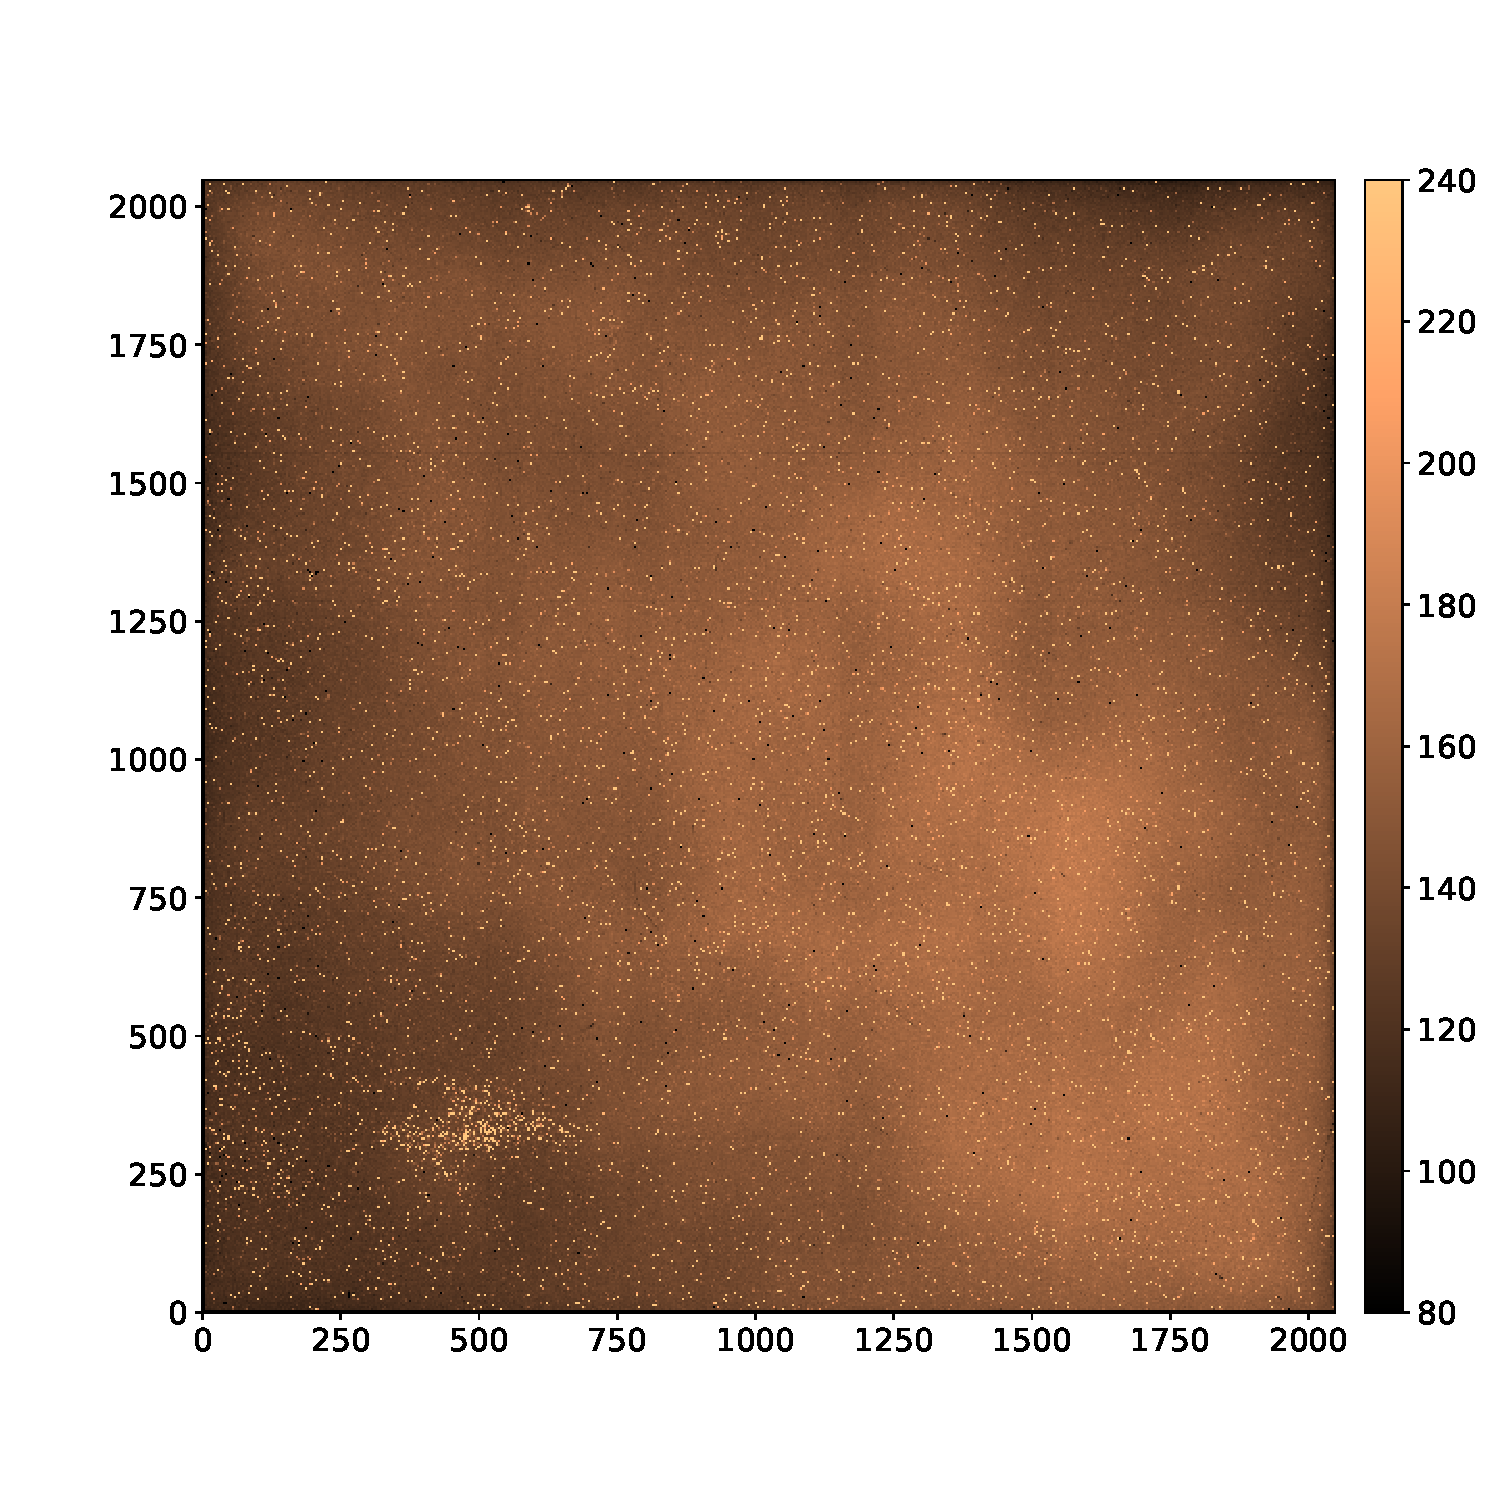
\includegraphics[width=1\linewidth]{dark}
  \caption{master dark}
  %\label{fig:sub2}
\end{subfigure}
\caption{result of the master dark recipe}
\label{fig:masterdark}
\end{figure}

\subsection{Detector flat}
At this step, the variation in sensitivity of the different pixels on the detector is measured. This can be done by using the extremely useful ability of the IFS to obtain flats with the shutter of the instrument closed and one of its internal calibration sources turned on. This means that the detector can be illuminated directly, which enables us to correct for the distortions of the detector itself. The distortions in the optical path are measured in the recipe that produces the instrument flat, described in the next paragraph. 
\bigskip

\begin{figure}[!b]
\centering
\begin{subfigure}{.48\textwidth}
  \centering
  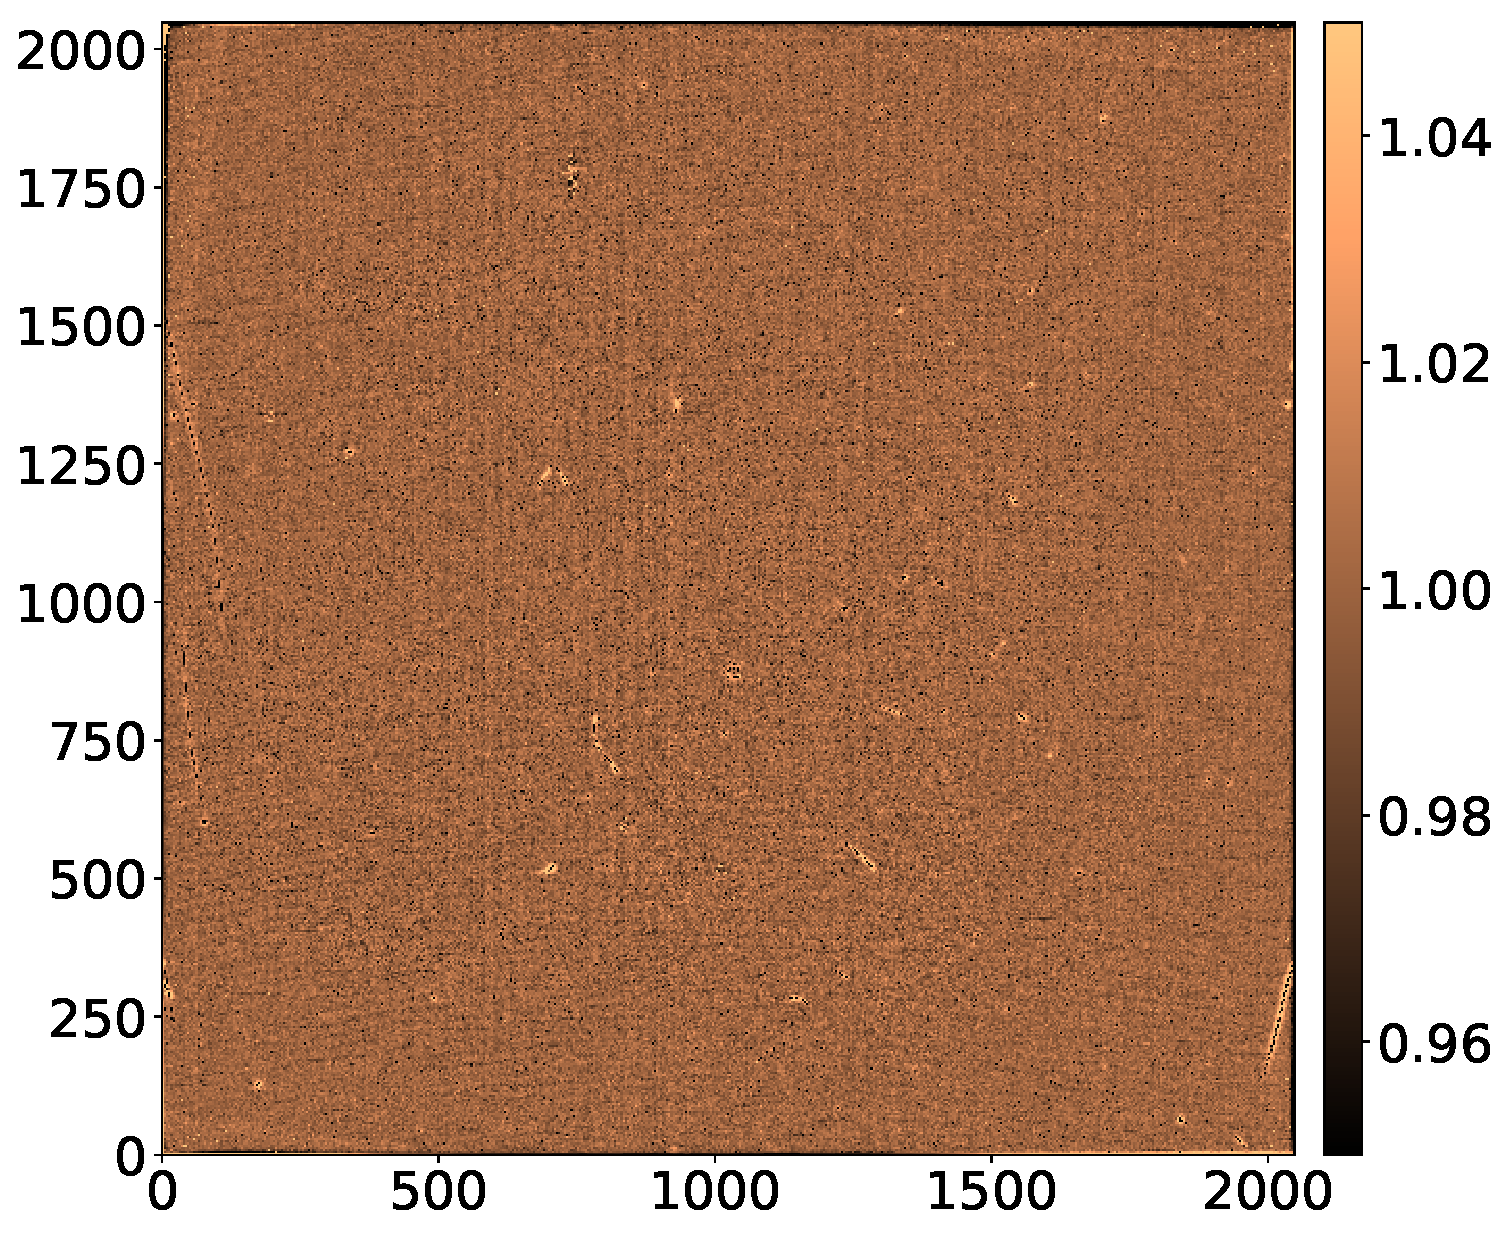
\includegraphics[width=1\linewidth]{masterdetectorflat}
  \caption{master detector flat}
  \label{fig:masterdetectorflat}
\end{subfigure}\hfill
\begin{subfigure}{.48\textwidth}
  \centering
  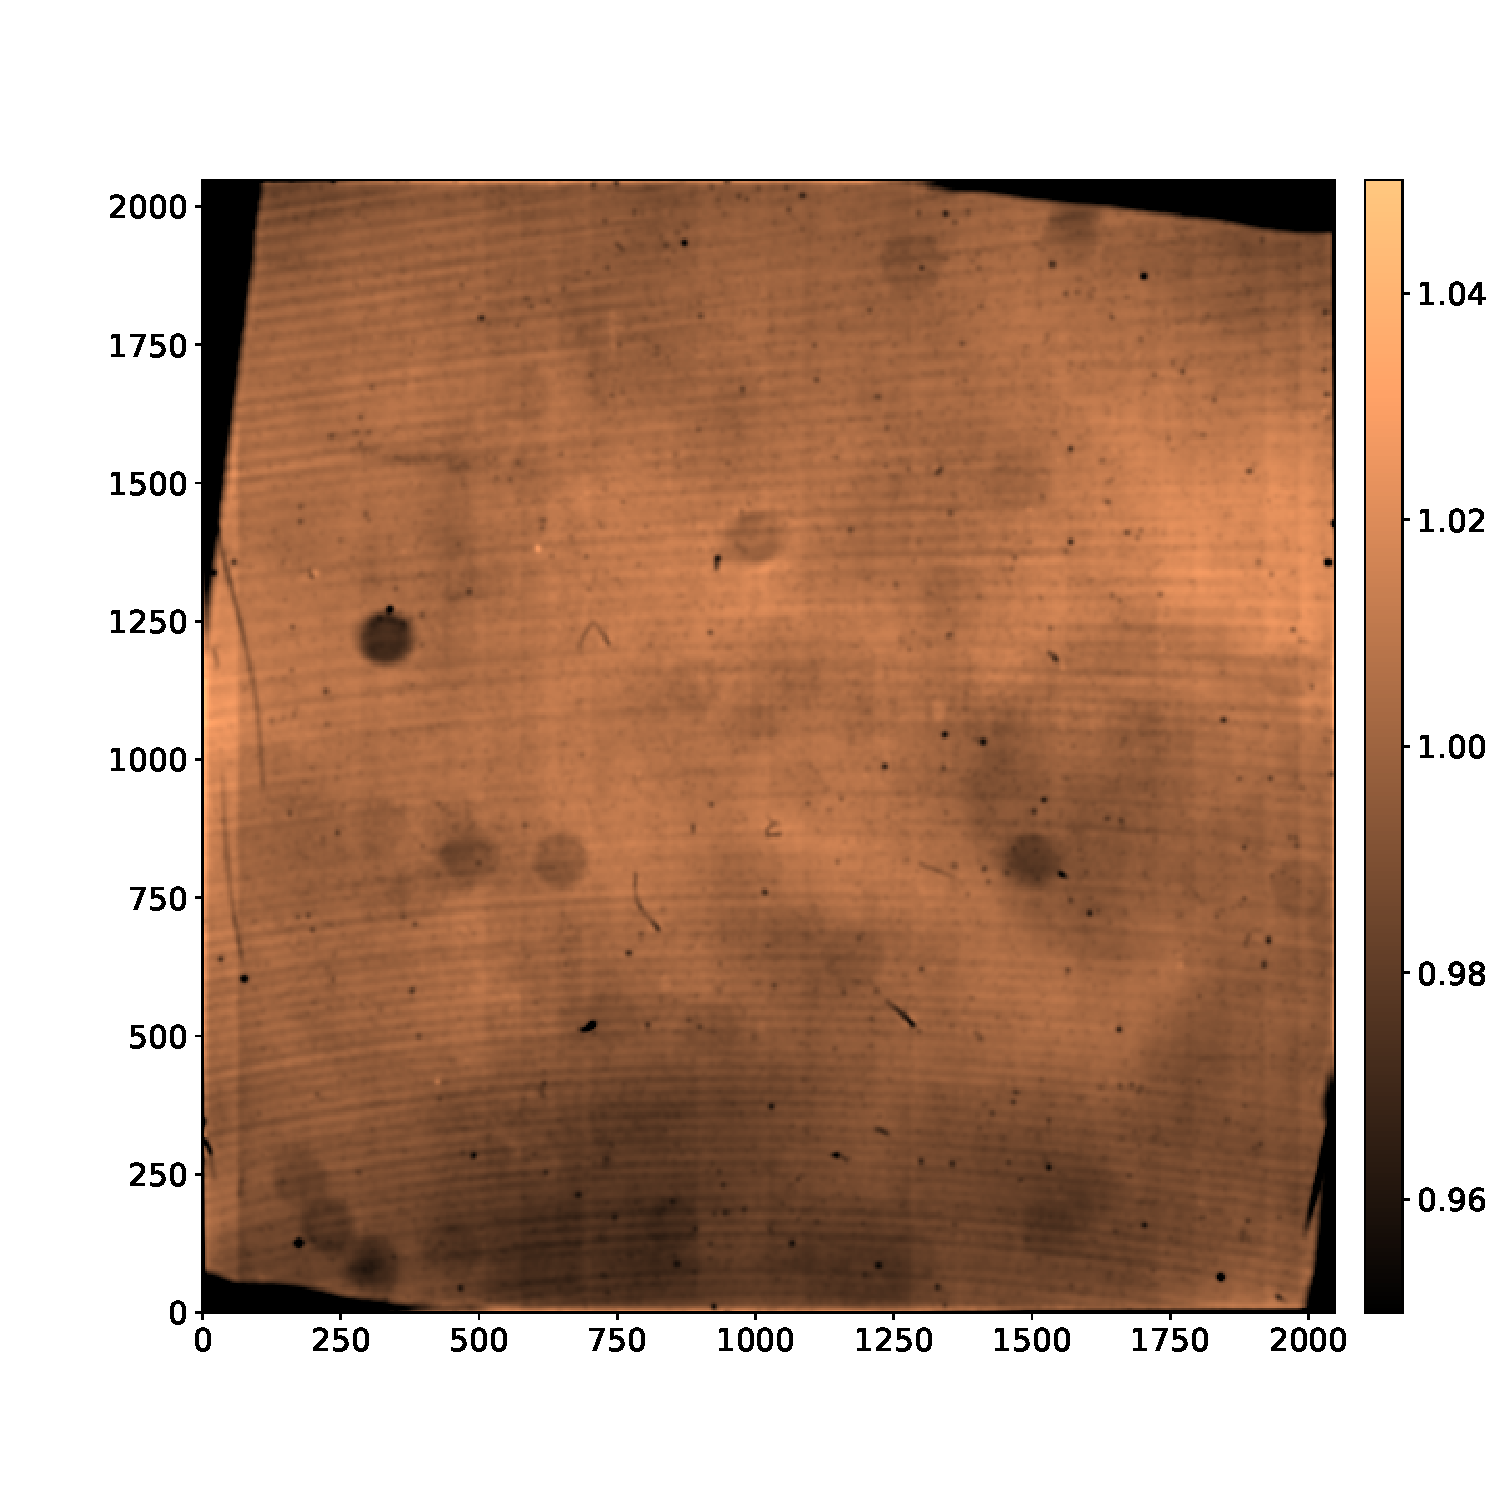
\includegraphics[width=1\linewidth]{largescaleflat}
  \caption{large scale flat}
  \label{fig:largescaleflat}
\end{subfigure}
\caption{result of the detector flat recipe}
%\label{fig:masterdark}
\end{figure}

Since the IFS uses a range of wavelengths, different detector flats are needed to calibrate all pixels properly. The recipe returns the master flat frames for the different lamps that are used. The best flat to use in the rest of the recipes are the master detector flats Figure \ref{fig:masterdetectorflat}. Large scale flats are master flat frames that are smoothed with a gaussian. On this images the large scale structures in pixel-to-pixel variation in the signal response of the detector get visible, such as ghosts. Large scale flats and pre-amplifier flats can be used as a calibration file for the actual detector flat recipe, but if they are not provided, they are created from the raw data. One of the large scale flats is illustrated in Figure \ref{fig:largescaleflat}

\subsection{Instrument flat}
\begin{figure}[!b]
\centering
\begin{subfigure}{.48\textwidth}
  \centering
  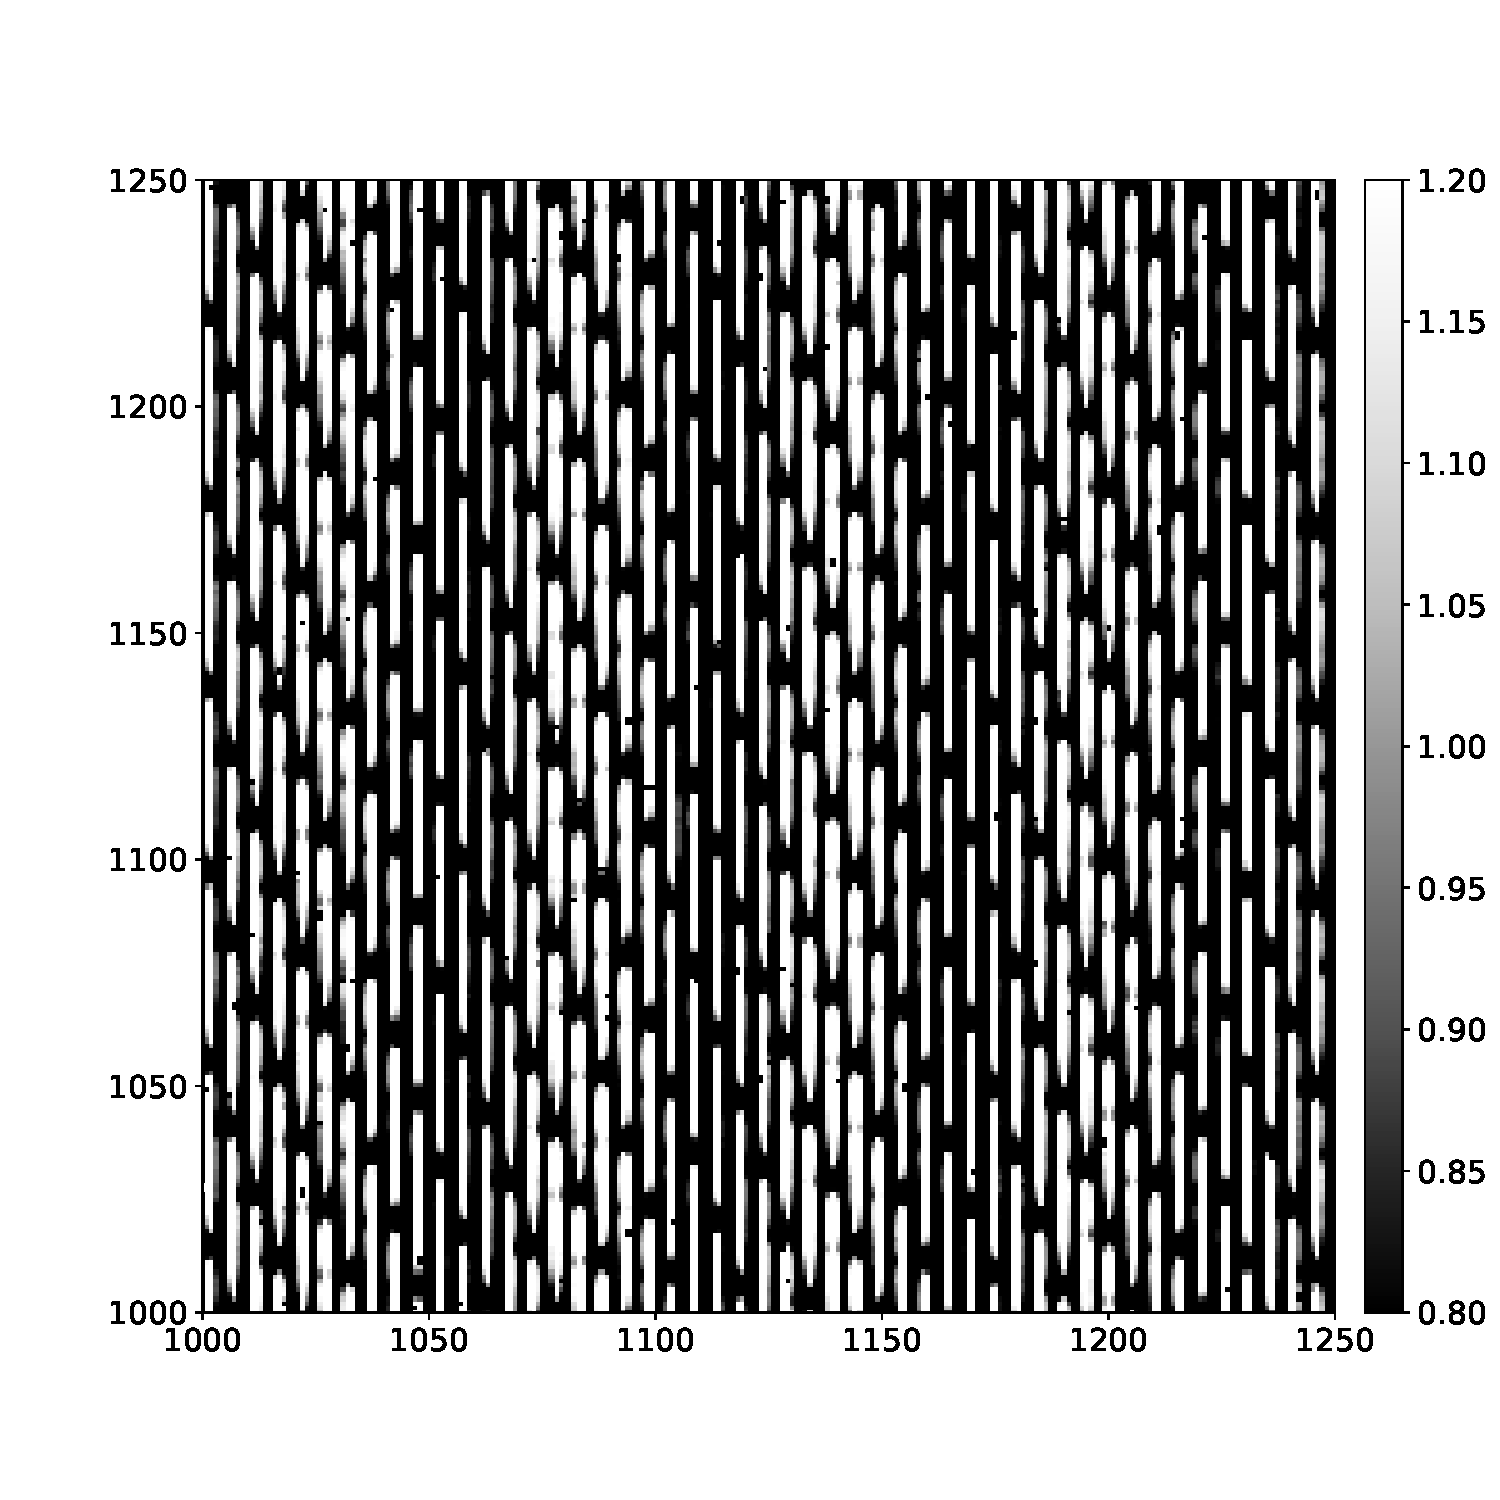
\includegraphics[width=1\linewidth]{instrumentflat}
  \caption{zoomed instrument flat}
  %\label{fig:preampflat}
\end{subfigure}\hfill
\begin{subfigure}{.48\textwidth}
  \centering
  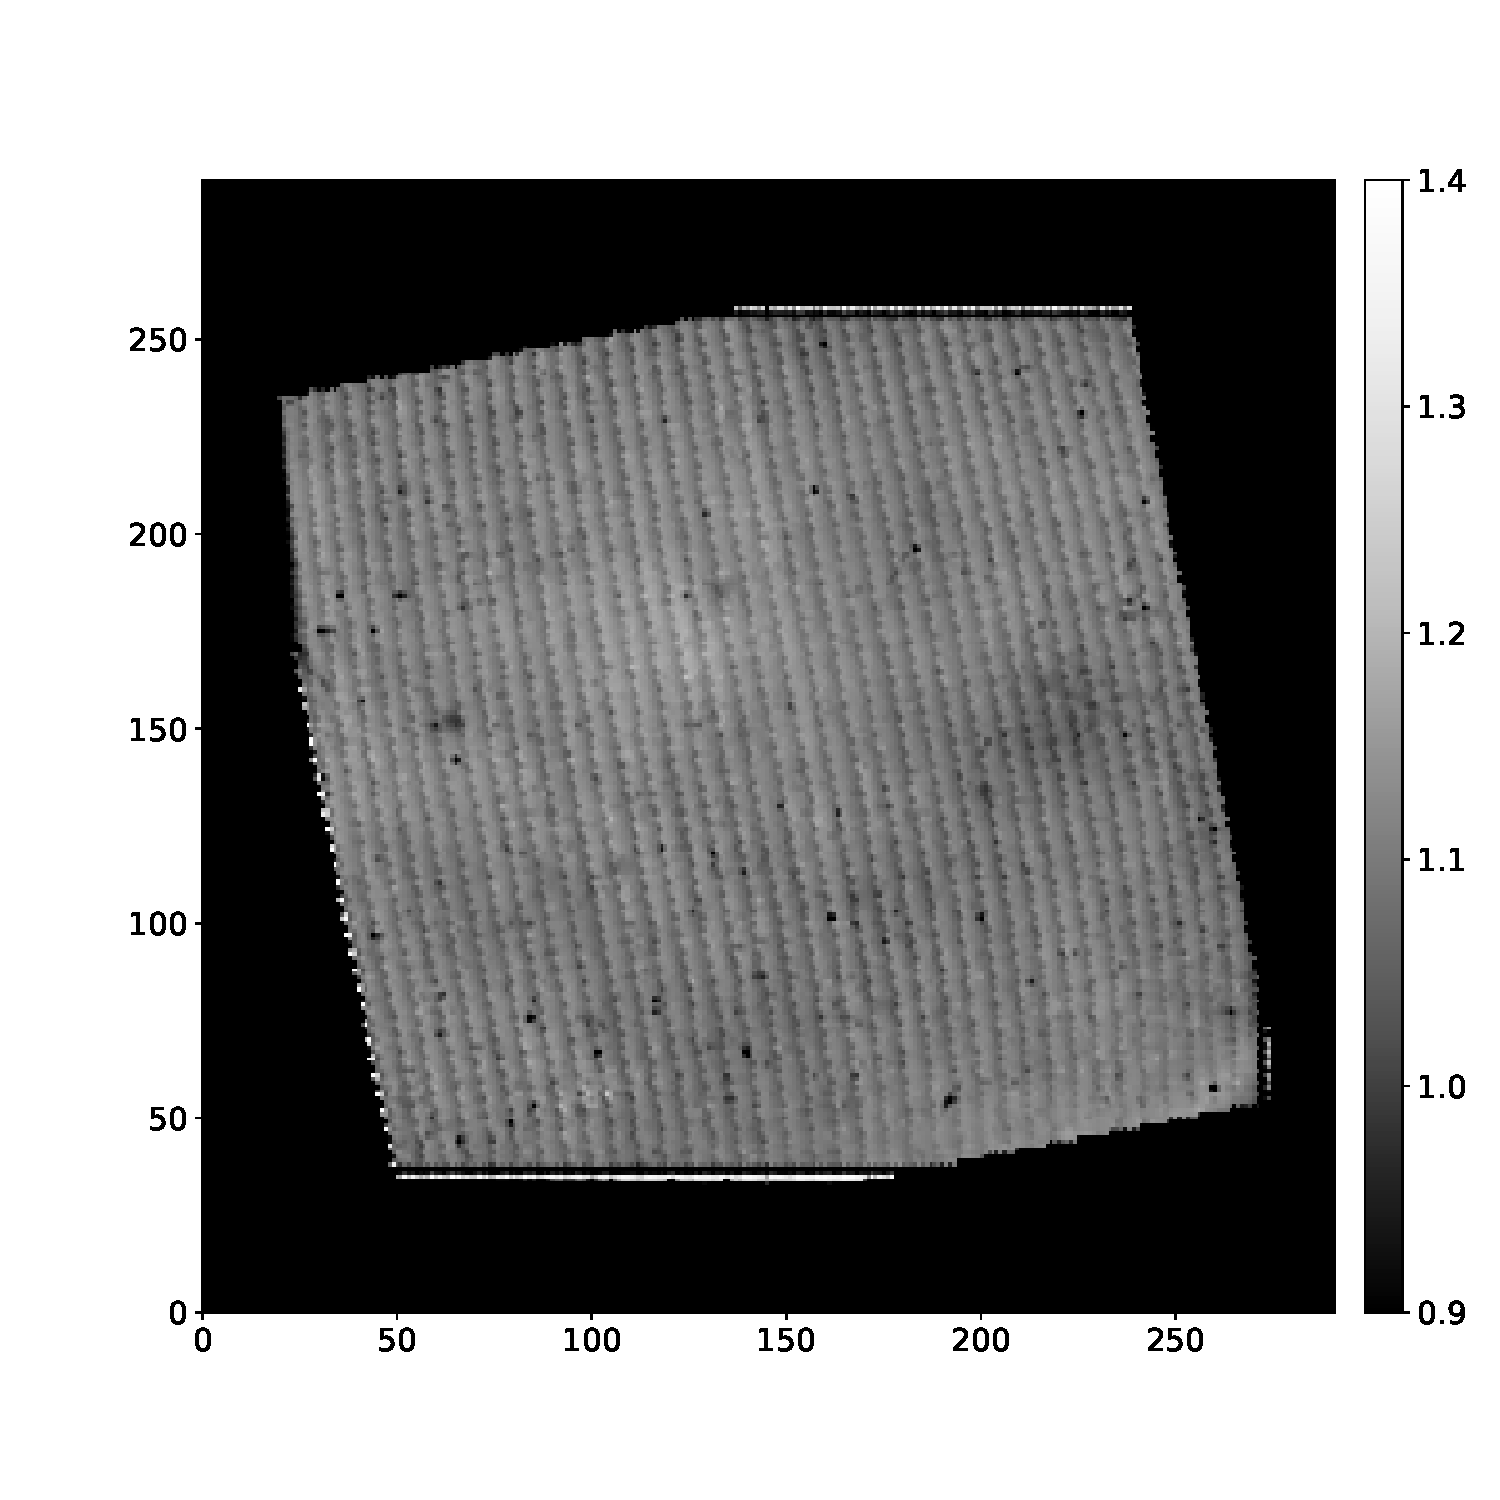
\includegraphics[width=1\linewidth]{IFU_flat}
  \caption{IFU flat}
  %\label{fig:largescaleflat}
\end{subfigure}
\caption{result of the instrument flat recipe}
\label{fig:instrumentflatrecipe}
\end{figure}
Instrument flats are obtained by taking a flat with three or four of the external calibration lamps switched on and is used to correct for the varying througput in the common path of the telescope and the instrument. After the dark subtraction, the flat field is divided by the detector flat, which removes the detector response. This recipe returns both an instrument master flat which is the combined and reduced flat field before removing the detector response and the response of the integral field unit (IFU), which is the flat field after removing the detector response. The first can be used only for calibrating other calibration data, the latter can be used to reduce science data. The IFU flat field can be produced only if a reduced wavelength calibration is given. The production of the instrument flat is already possible with the positions of the spectrums only and is used to correct for the distortion of the lenslet grid in the wavelength calibration. The IFU flat does not give all pixels a sensitivity value, but assuming that most of the spatial distortion is due to the lenslet grid, the recipe returns the response of each individual lenslet. It gives a median value for all pixels in the same spectrum. This is why the IFU flat contains a typical stripe like feature. Both the IFU flat and the instrument flat are shown in Figure \ref{fig:instrumentflatrecipe}. 

\subsection{Positioning spectra}
\begin{figure}[!b]
\centering
\begin{subfigure}{.48\textwidth}
  \centering
  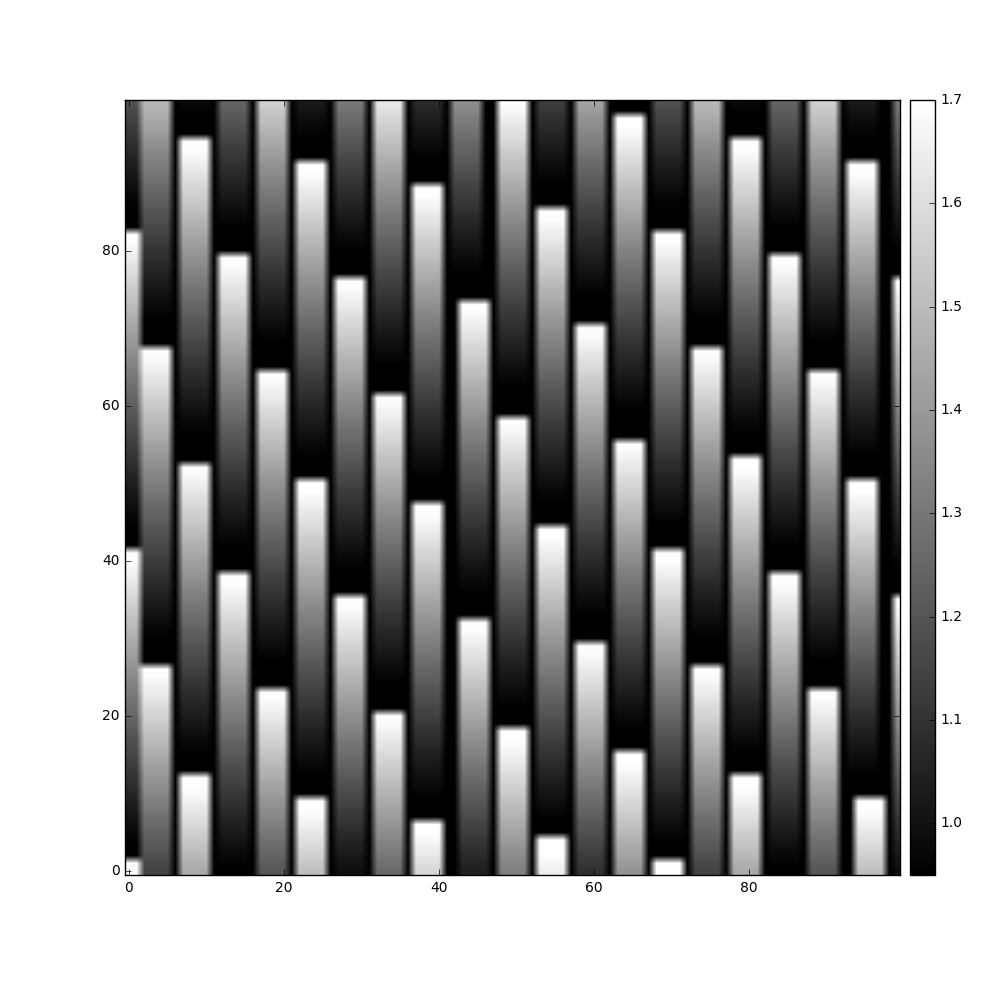
\includegraphics[width=1\linewidth]{specpos}
  \caption{zoomed positions of the spectra}
  \label{fig:specpos}
\end{subfigure}\hfill
\begin{subfigure}{.48\textwidth}
  \centering
  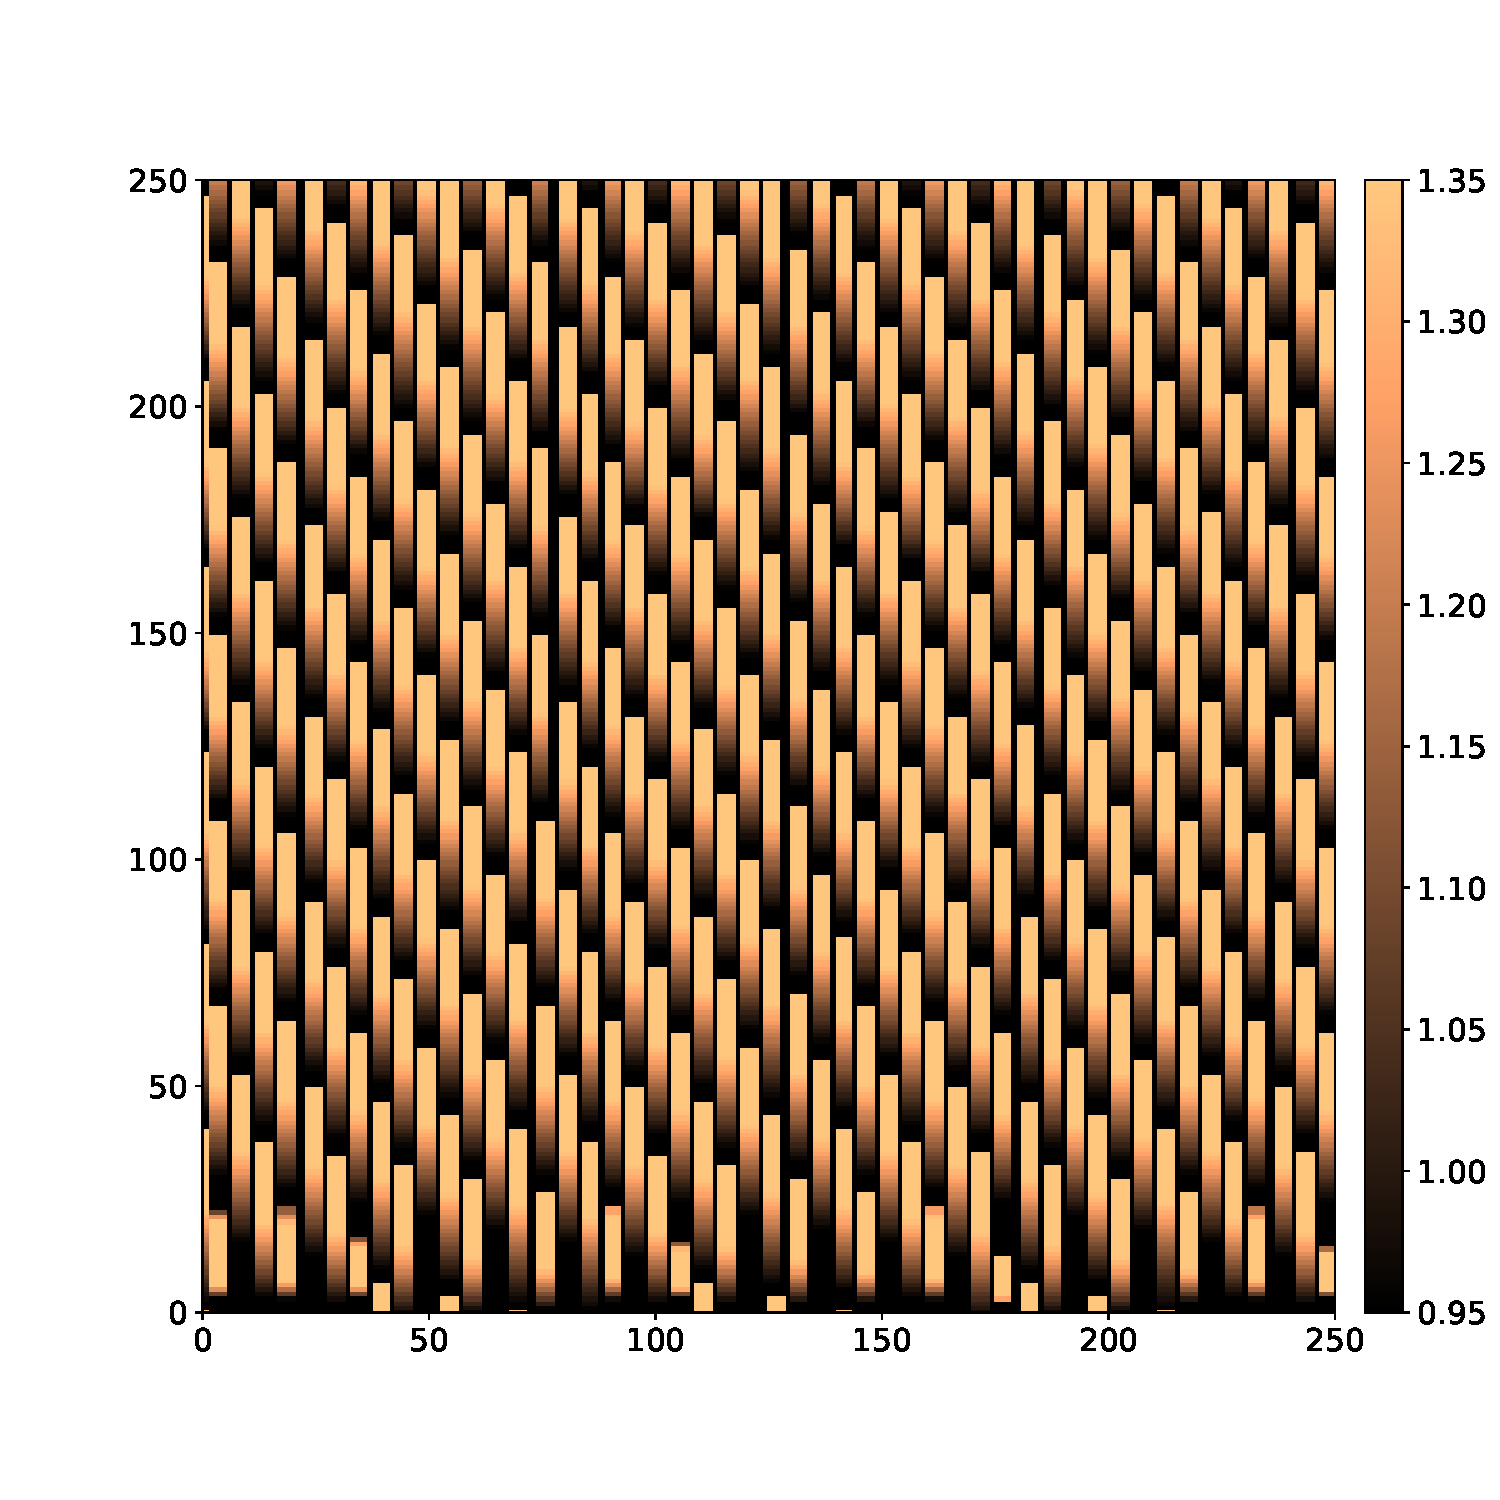
\includegraphics[width=1\linewidth]{wavecalib}
  \caption{zoomed wavelength calibration}
  \label{fig:wavecal}
\end{subfigure}
\caption{}
%\label{fig:masterdark}
\end{figure}

The spectra positioning recipe determines the exact position of the different spectra on the detector with an accuracy of about 4 $\mu m$, which corresponds to 0.2 pixels on the detector \citep{Desidera2008}. This is enough to build a map with the location of the spectra, associating each pixel to an individual lenslet. It associates pixels with wavelengths according to a lenslet model. Note that this is a non-linear model, as is noticeable in \ref{fig:specpos}. Each pixel in this image has the value of the corresponding wavelength in micron. This model is just a good guess, the exact wavelength can be obtained by running the wavelength calibration. The seperation between the positioning of the spectra and the wavelength calibration makes the positioning of the spectra much better, which is the reason why they have split these steps in two different recipes. The raw calibration data for the spectra positioning recipe is obtained by illuminating the instrument with an external white calibration light source. A zoomed piece of the spectra positioning image is shown in Figure \ref{fig:specpos}

\subsection{Wavelength calibration}
The wavelength calibration recipe refines the wavelength of the different pixels, by using data that is obtained by illuminating the instrument with three or four external lasers, emitting at 0.9877, 1.1237, 1.3094 and 1.5451($\mu m$). The recipe tries to fit a spectrum on the positions that are determined in the spectra positioning recipe. Note that if a part of the spectrum does not fit on the detector, the recipe is unable to fit a spectrum, as illustrated in Figure \ref{fig:wavecal}.

\subsection{Science reduction}
In the science reduction recipe the science frames are finally calibrated. This recipe needs all the output of the different calibration recipes as input alongside the raw science frames, in order to reduce the data properly and asign pixels of the detector to pixels of the result in the end: a 39x291x291 datacube.

\section{Post-processing methods}
After the basic science reduction, the disk around the star is still not visible to the naked eye, because of the bright stellar PSF that dominates the image. Post processing techniques, based on subtracting a model of the stellar PSF from the data were needed to recover the disk signal the best. Three different methods are used to make a model for the stellar PSF: angular differential imaging (ADI), spectral differential imaging (SDI) and reference star differential imaging (RDI). But before constructing a model for the PSF, the data needs to be centered correctly.

\subsection{Centering}
The telescope is calibrated such that the star is about in the center of the image, but there is always a slight offset. Center frames can be used to determine the center of the images on a level of up to tenths of a pixel. These center frames are science frames containing four artificial satellite spots, created by the adaptive optics system, with the center of the star exactly in the middle of the four satellite spots, as illustrated in Figure \ref{fig:centerframe}. These center frames are usually taken before, during and after the science run to be able to correct for small changes of the position during the run.
\begin{figure}[!t]
\centering
\begin{subfigure}{.48\textwidth}
  \centering
  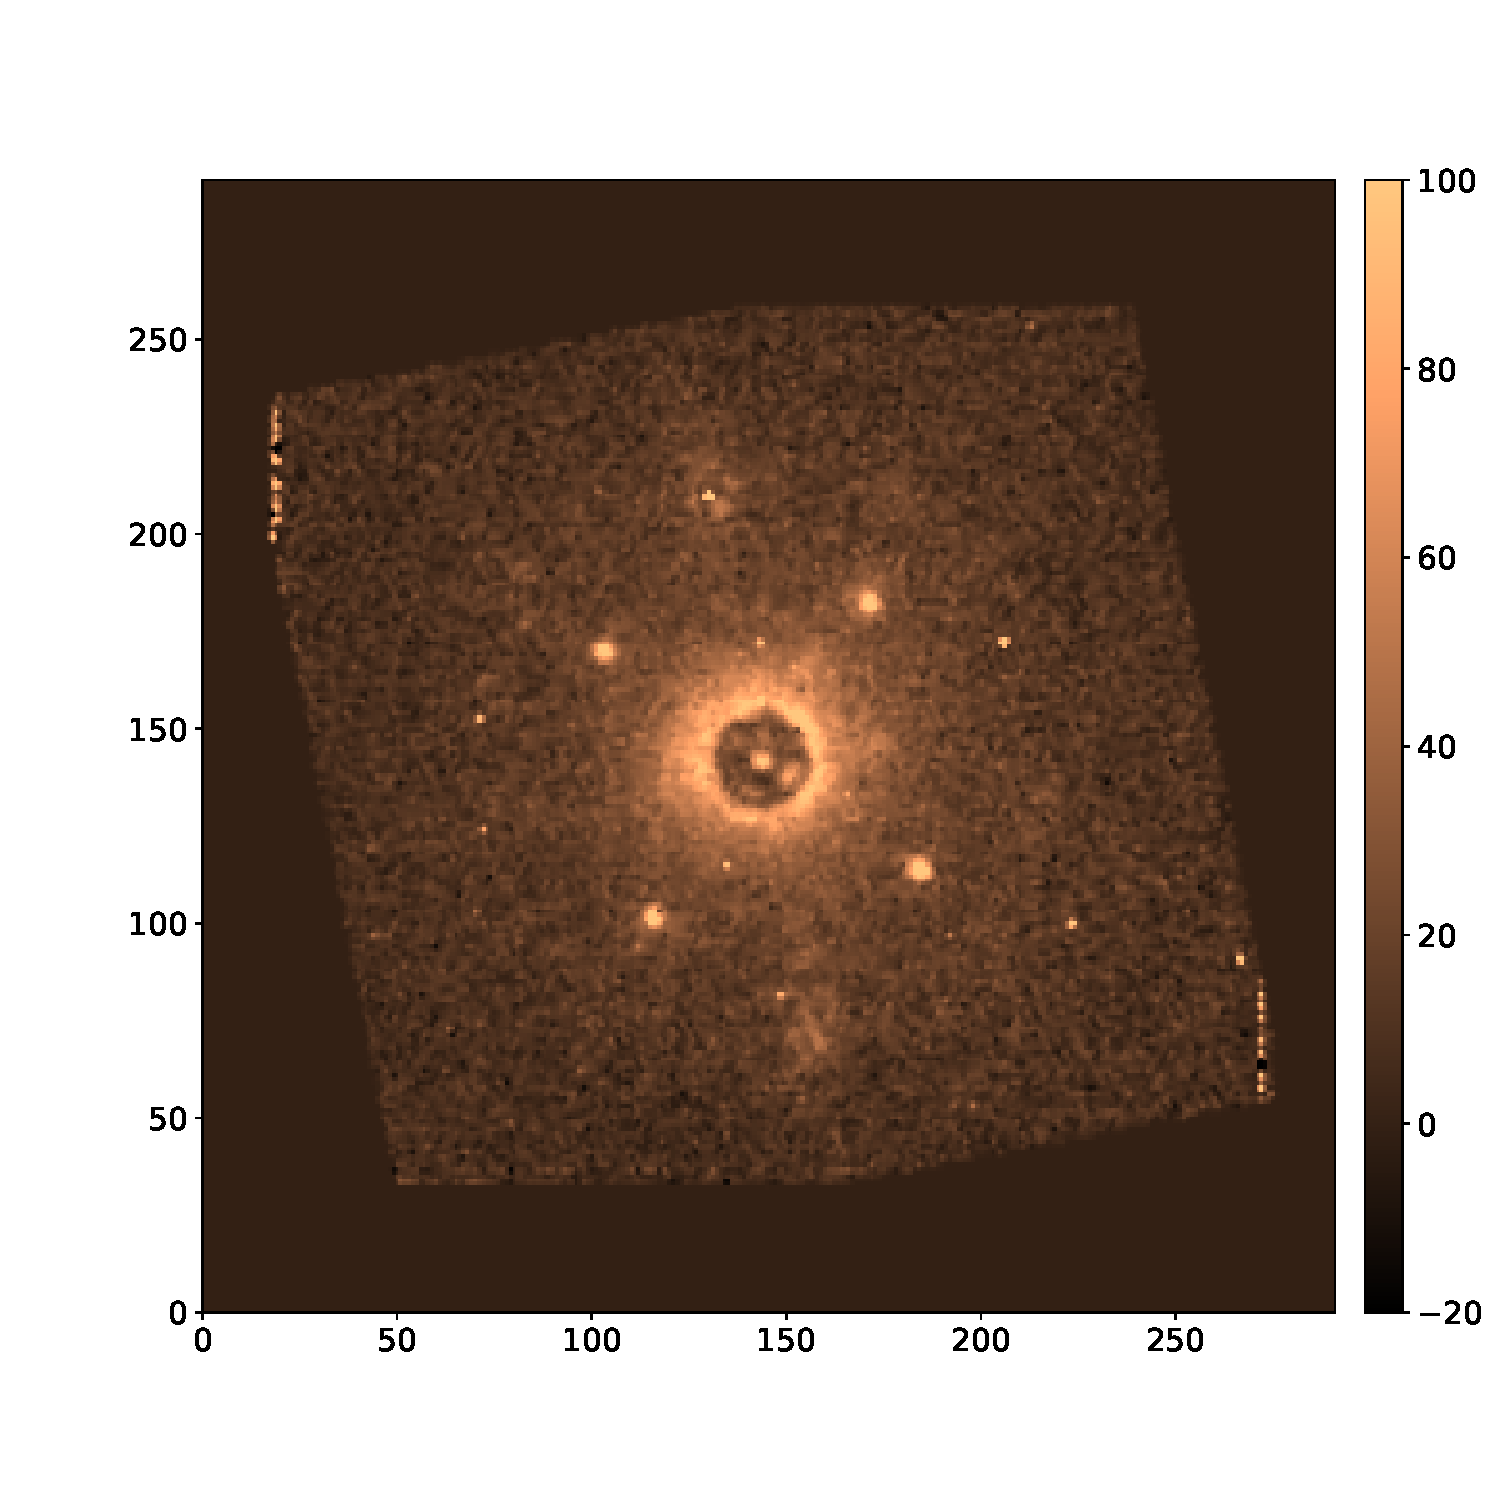
\includegraphics[width=1\linewidth]{centerframe}
  \caption{one of the 39 wavelength slices of a reduced center exposure\\}
  \label{fig:centerframe}
\end{subfigure}\hfill
\begin{subfigure}{.48\textwidth}
  \centering
  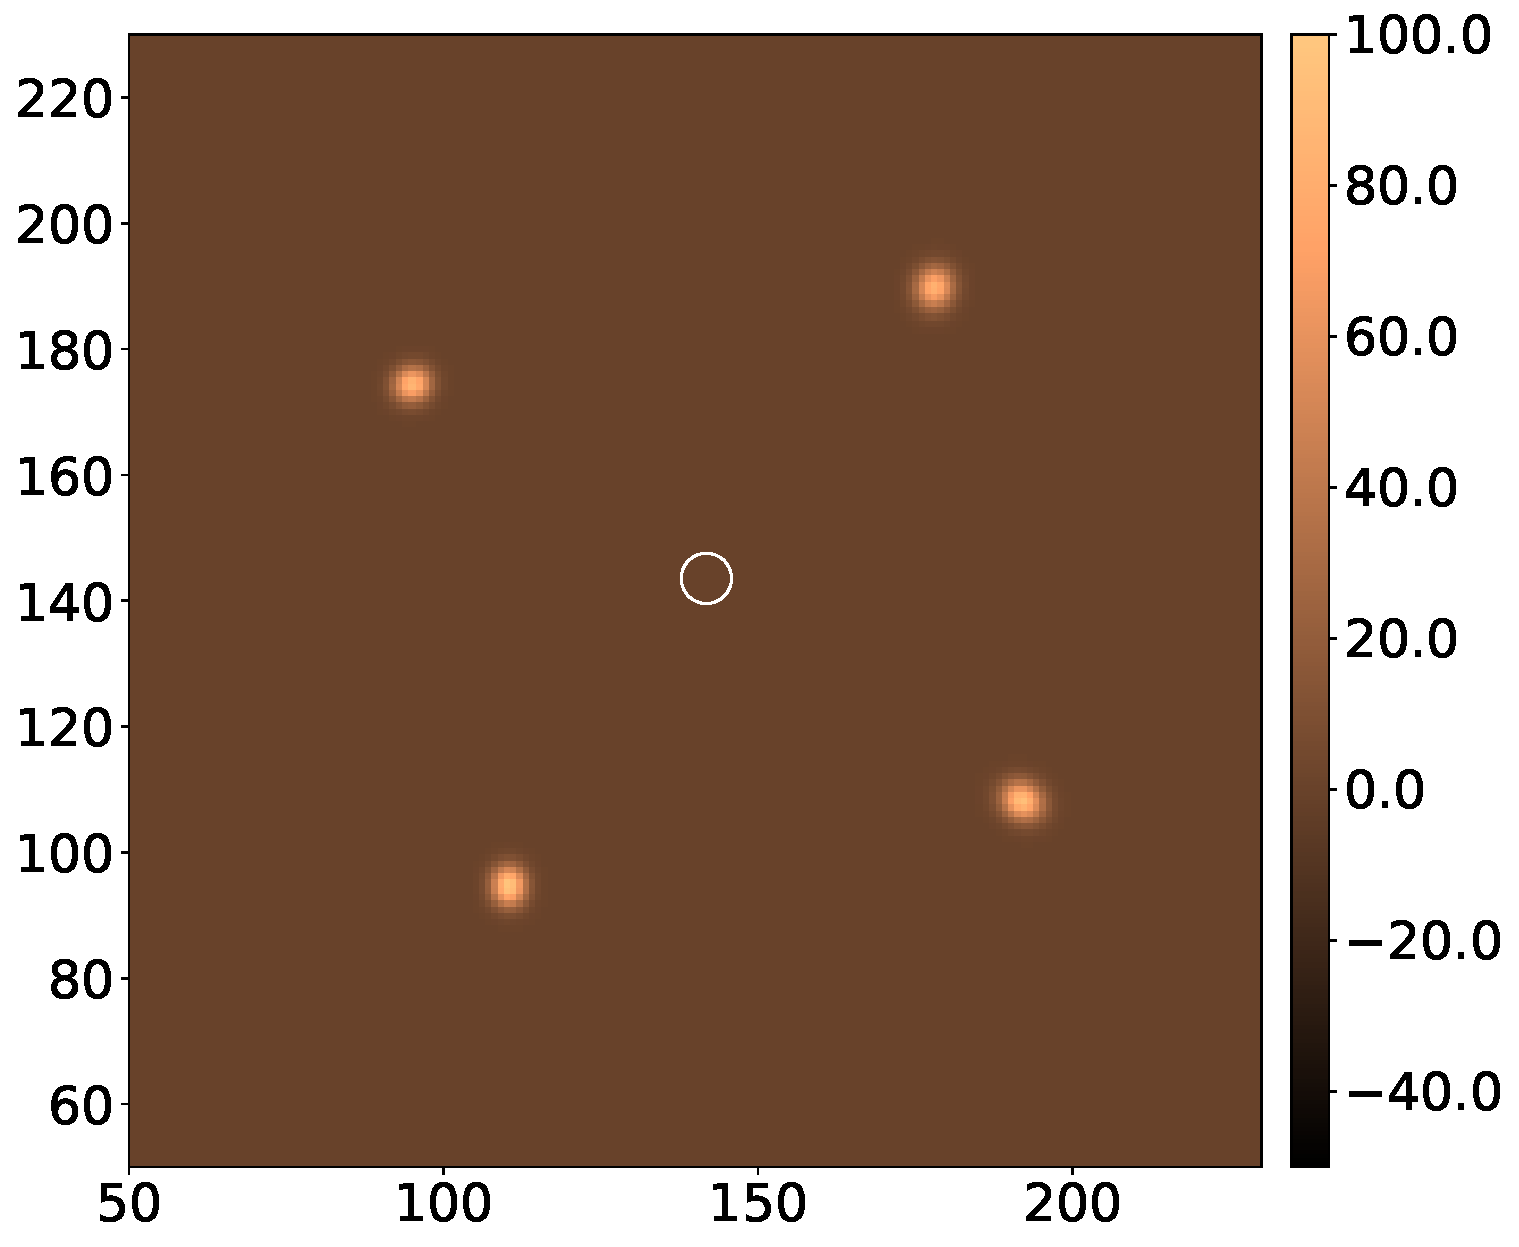
\includegraphics[width=1\linewidth]{centermodel}%
  \caption{model of the four satellite spots with the center of the star marked with a white circle}
  \label{fig:centermodel}
\end{subfigure}
\caption{results of the centering routine: four gaussians are fitted over the satellite spots in order to determine the exact position of the center of the frame.}
%\label{fig:masterdark}
\end{figure}

\begin{figure}[!b]
\centering
\vspace{-0.4cm}
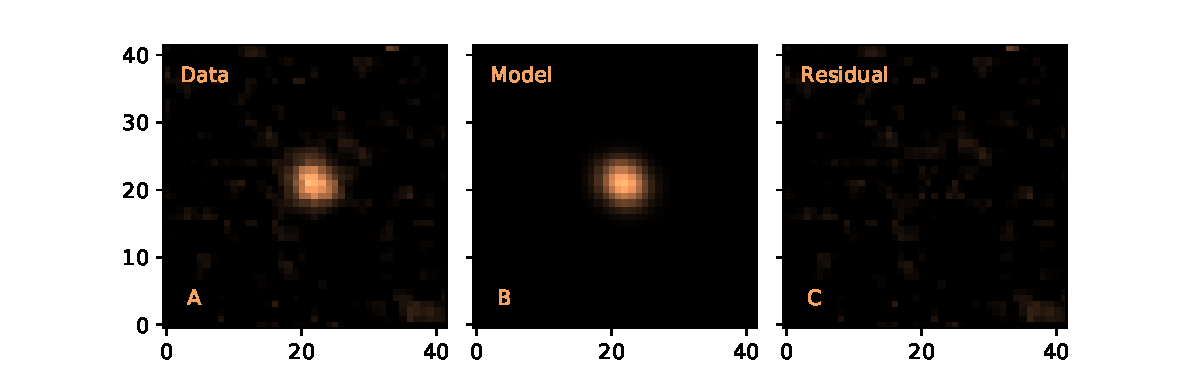
\includegraphics[width = \textwidth]{resultmodel}
\caption{\textbf{A:} one of the raw satellite spots, \textbf{B:} model of the satellite spot,\\ \textbf{C:} residual after subtracting the model of the data} 
\label{fig:resultmodel}
\end{figure}
\bigskip
Center frames are reduced in the same way as normal science frames, using the same dark and flat frames. The image is first smoothed with a gaussian with a standard deviation of 25 that filters all the high frequency noise out and leaves a clean image of the four satellite spots. After that a single gaussian is fitted over each of the four satellite spots and a model is created for the combined satellite spots. The position of the center can be determined from the positions of the fitted gaussians. 
\bigskip

The fit of all the satellite spots on the centerframes were good, leaving almost no residual signal after subtracting the model from the data, as illustrated in Figure \ref{fig:resultmodel}. The positions of the satellite spots are accurately measured with an uncertainty on the fit of each individual satellite spot between 0.40 and 0.45 pixels for both the x and y coordinate. Since we have six independent distances, four with an x component and four with a y component, the uncertainty on both the x and y coordinate of the center is 0.2 pixels.

\subsection{Angular differential imaging}
\begin{figure}[!b]
\centering 
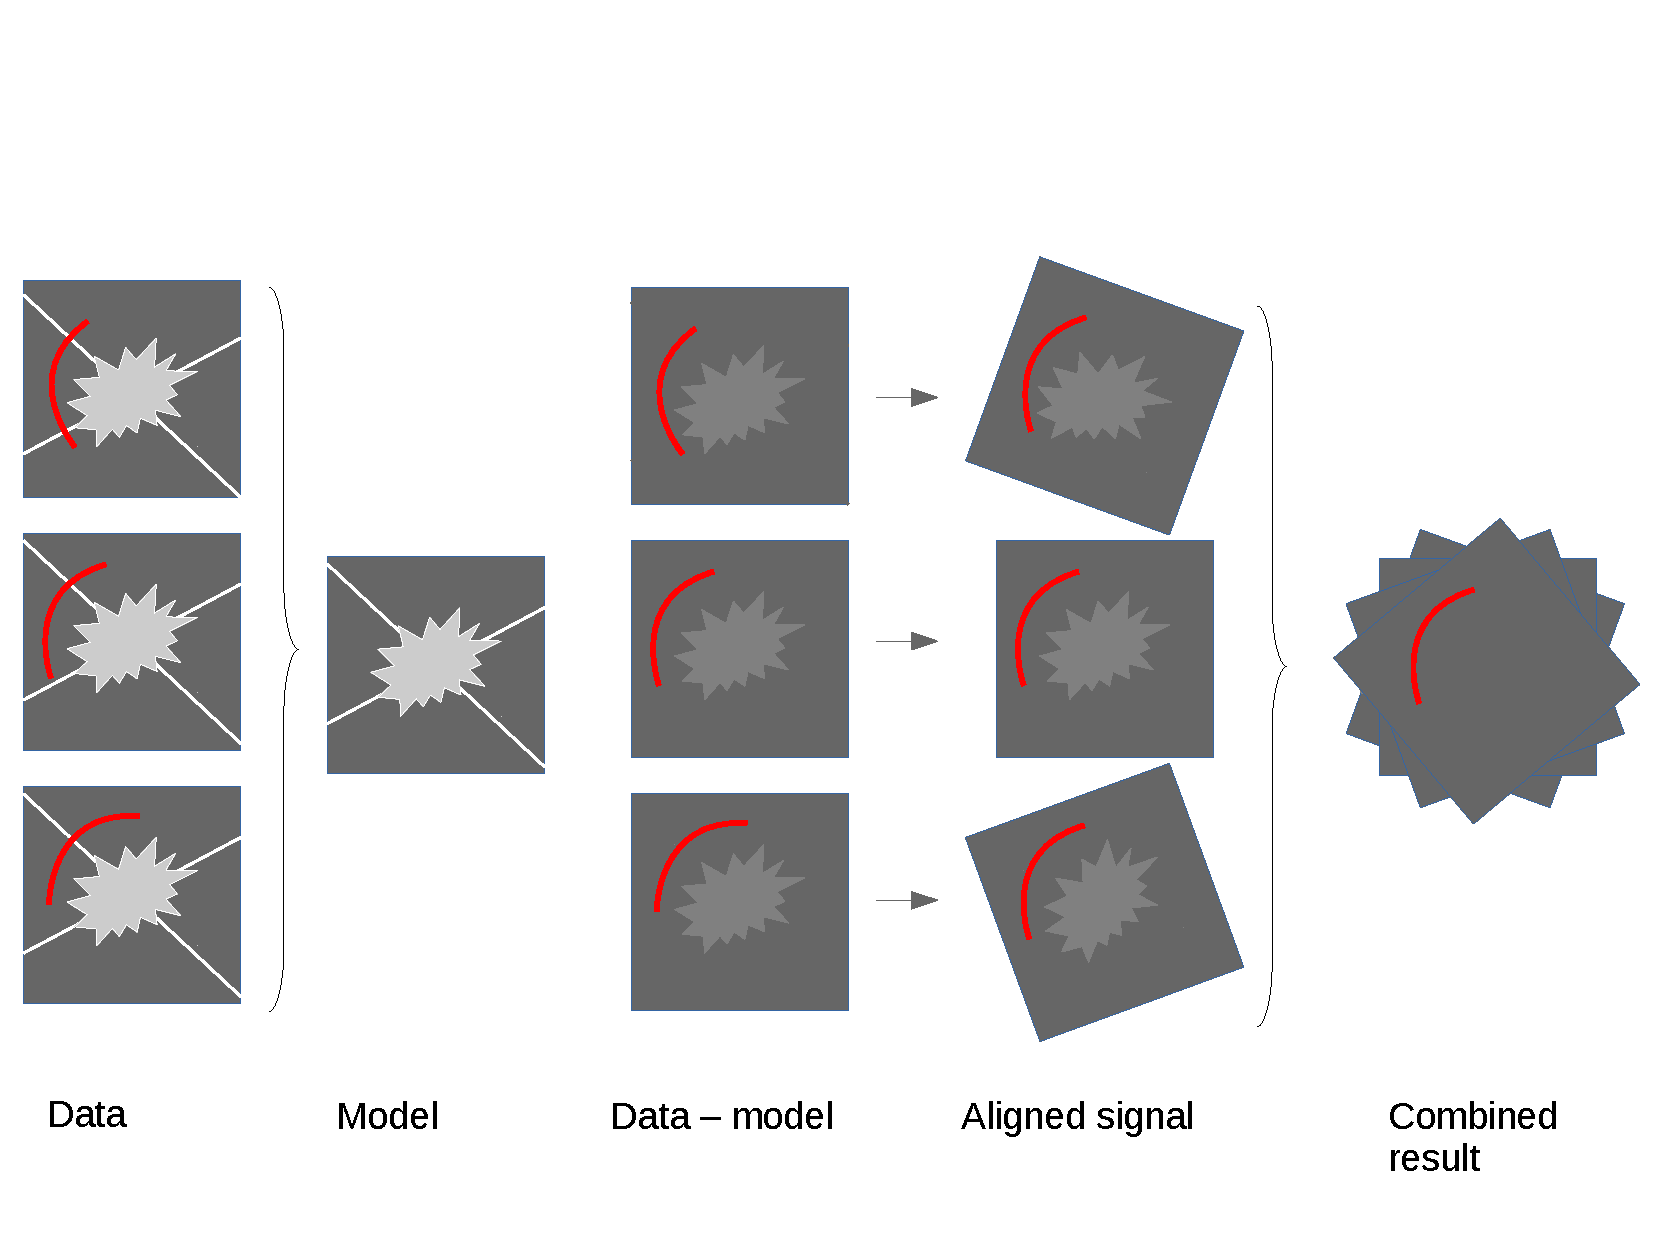
\includegraphics[trim={0cm 1cm 0cm 4cm},clip,width = \textwidth]{adiexplanation}
\caption{Explanation of the ADI procedure. Data with a certain amount of field rotation is median combined into a model for the fixed stellar PSF, with the least amount of disk signal in it, which is subtracted from the original data, leaving after combination a resulting image of the disk with high SNR} 
\label{fig:adiexplanation}
\end{figure}

ADI is a post-processing method that constructs a model for the stellar PSF by using the rotation of the field during the night \cite{Marois2006}. The star can be considered as a point source that does not change under rotation. This implies that the stellar PSF remains stable on the detector and at the same orientation all the time, since we observe in pupil stabilized mode. Astrophysical signal around the primary star, however, is rotating by the amount of the change in parallactic angle. The total field rotation during the observation run was 69 degrees, in 16 different exposures, meaning that the signal has changed significantly on the detector over time. Taking the median per pixel, per wavelength over the whole time should hence give a model for the PSF of the star, with the least amount of disk signal in it. Subtracting this model from each individual frame and realigning the disk singal with each other by rotating each frame with the known rotation of the field gave good results. A detailed explanation of the ADI procedure is also given in Figure \ref{fig:adiexplanation}.
\bigskip

\begin{wrapfigure}{R}{0.6\textwidth}
\centering
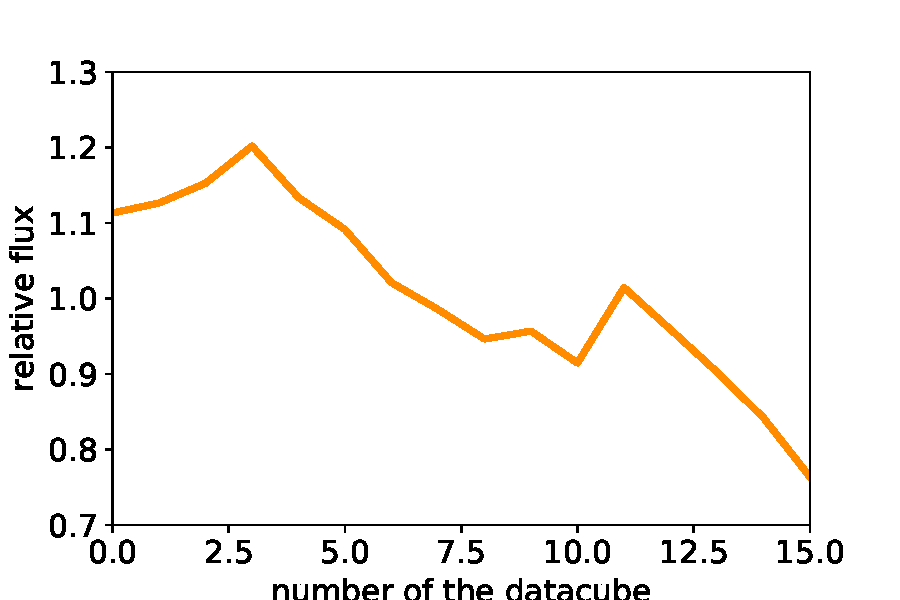
\includegraphics[width = 0.56\textwidth]{aonorm}
\caption{Relative flux of the different datacubes over time. This is used to normalize the data between different exposures.}
\label{fig:aonorm}
\end{wrapfigure}

Since the data was taken with more than an hour between the first and last exposure, the flux of the object on the detector changes. This is due to changes of conditions in the sky during the night and in the performance of the AO system. To correct for this, the median amount of flux in an annulus that grows linearly in size with wavelength is measured. This annulus has an inner radius that is located in each frame just outside the outer ring of flux that is created by the coronagraph. Since the PSF scales with $ \propto\lambda/D$, the radii of the annulus has to change for different wavelengths, to measure the flux in the same region of the PSF. The measured flux over wavelength is illustrated in Figure \ref{fig:aonorm}. With this relative flux the PSF of the star in different exposures can be normalized so that it is correctly subtracted in each frame in the procedure. After the subtraction and before combination of the different frames, the normalization is reversed, so that the disk signal is not amplified in certain frames.

\subsection{Spectral differential imaging}
\begin{figure}[h]
\centering 
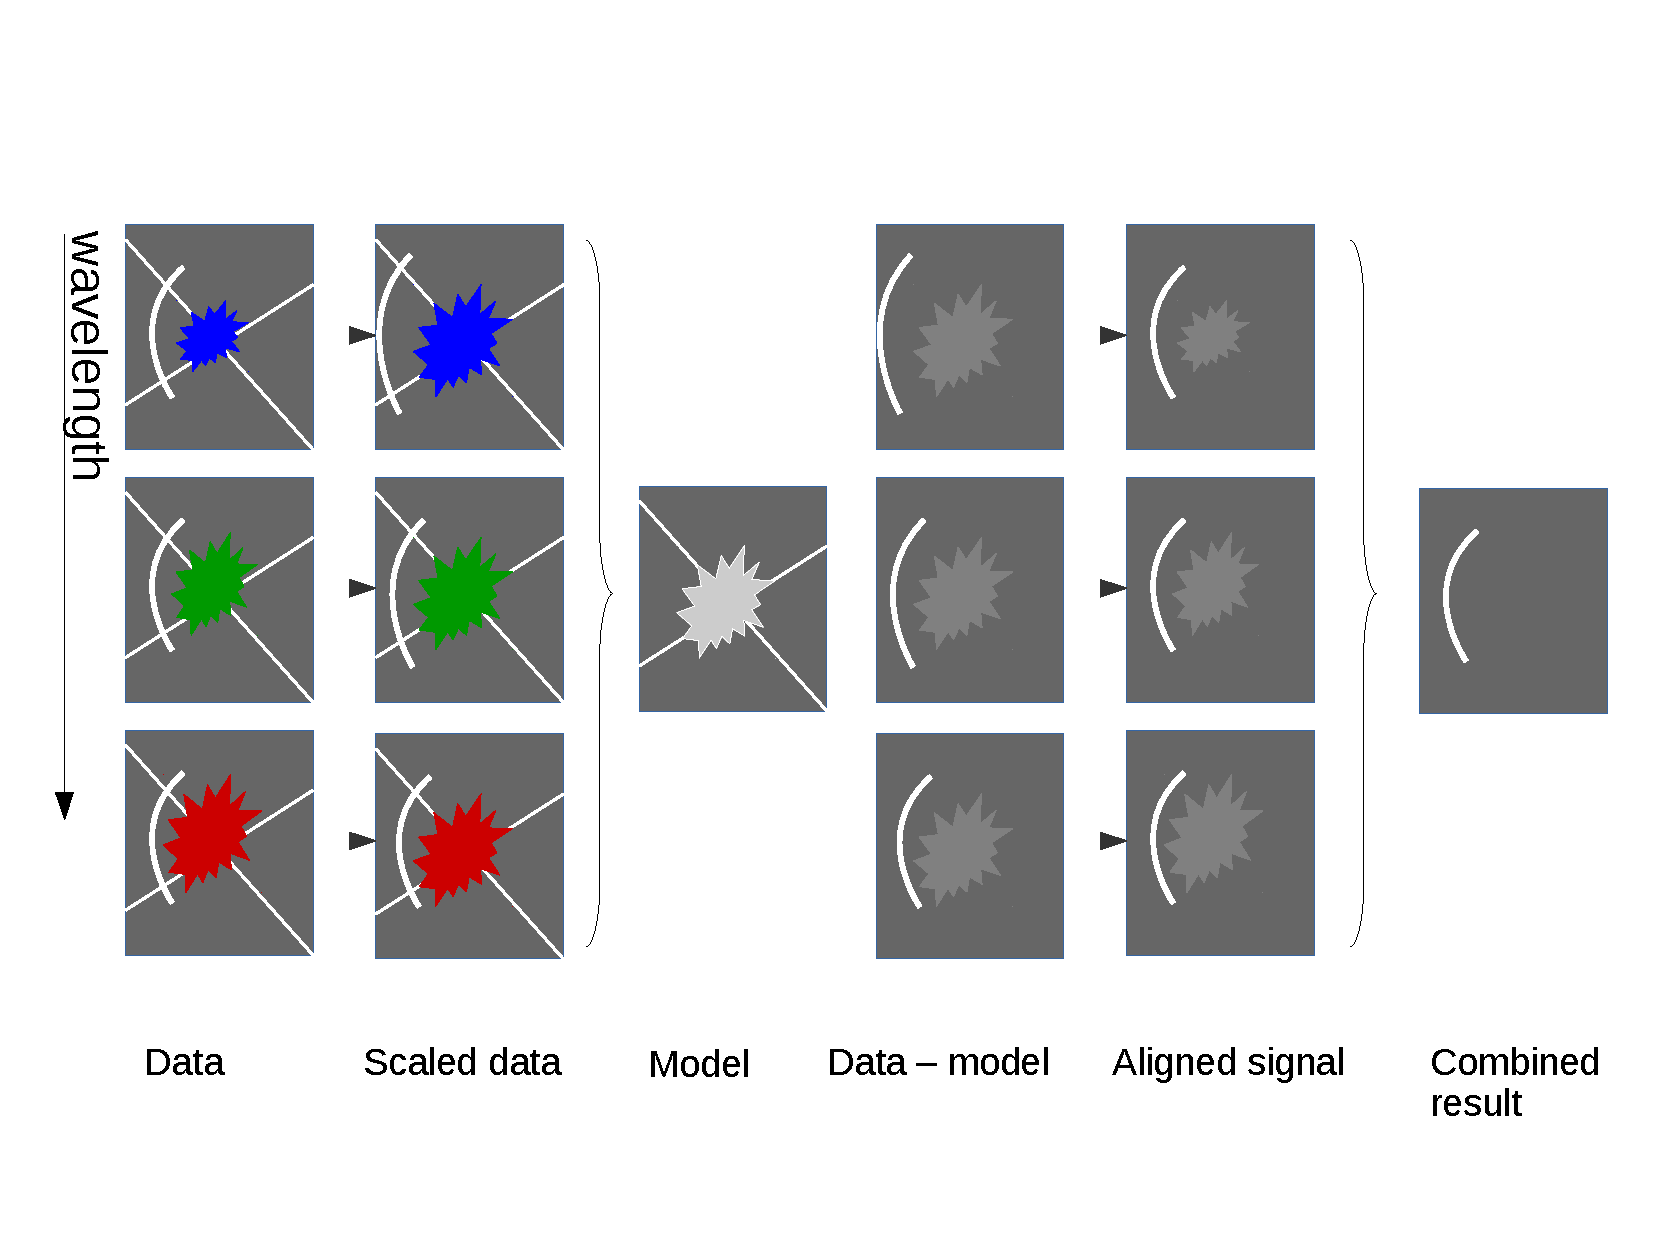
\includegraphics[trim={0cm 1cm 0cm 3cm},clip,width = \textwidth]{sdiexplanation}
\caption{Explanation of the SDI procedure. Data of different wavelength channels have a different PSF size, while the disk signal is fixed. Median combination of the different spectral channels, after scaling all the images such that the PSFs are the same size in each channel, gives a model for the stellar PSF with the least amount of disk signal in it. This model is subtracted from the data, after which the images are rescaled to their initial size, which results in an image of the disk with high SNR after median combination of the different channels.} 
\label{fig:sdiexplanation}
\end{figure}

SDI is a post-processing method that constructs a model for the PSF of the star by use of the wavelength dependency of the PSF. The PSF of a star scales with $ \propto\lambda/D$, which means that the resolution and hence the scale of the PSF is directly proportional to the wavelength. We expect therefore that the PSF of the star increases linearly with wavelength. The signal of the disk however does not. This means that this should leave us with a model for the PSF, after taking a median over all 39 spectral channels, that {\parfillskip0pt\par}


\begin{wrapfigure}{!bR}{0.6\textwidth}
\centering
%\vspace*{-0.5cm}
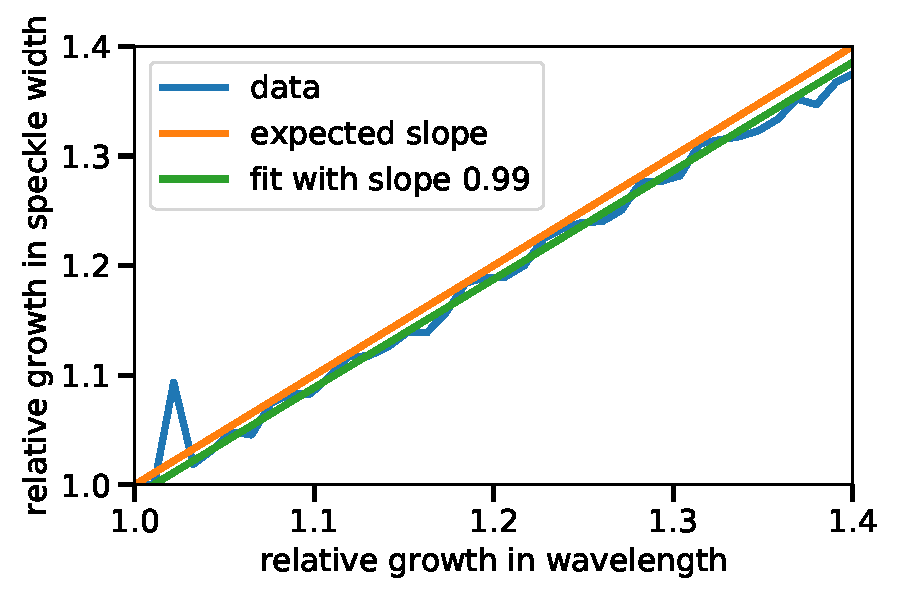
\includegraphics[width = 0.58\textwidth]{specklegrowth}
\caption{Relative growth in the size of the PSF of the star versus wavelength. Note that the data follows almost exactly the expected slope.}
\label{fig:specklegrowth}
\vspace*{-0.5cm}
\end{wrapfigure}

\noindent
does contain the least amount of disk signal. A detailed explanation is also given in Figure \ref{fig:sdiexplanation}.
\bigskip

In order to check if the scale of the PSF is directly proportional to the wavelength, we measured the distance between the different artificially created satellite spots in the center image, using the same model as in the frame centering procedure. The result of this measurement and the expected slope are plotted in Figure \ref{fig:specklegrowth}. This result indicates that the size of the PSF is indeed directly proportional to the wavelength, which means that the throughput of the instrument does not spatially distort different wavelengths and that the wavelength calibration and positioning of the spectra is done correctly.
\bigskip

Just as in the angular differential imaging, the data needs to be normalized before we take the median in order to get a good model of the PSF in each spectral channel. Since the throughput of the atmosphere, the instrument and the common path of the telescope is wavelength dependent, we had to normalize the flux in the different spectral channels. Our first try was to average the amplitude of the four fitted gaussians over the satellite spots in the center frames. Secondly, we tried to measure the flux in a fixed annulus around the center, after scaling the different spectral channels so that the PSFs lined up. The different scaling factors are illustrated in Figure \ref{fig:throughputnorm}.
\bigskip

\begin{wrapfigure}{R}{0.6\textwidth}
\centering
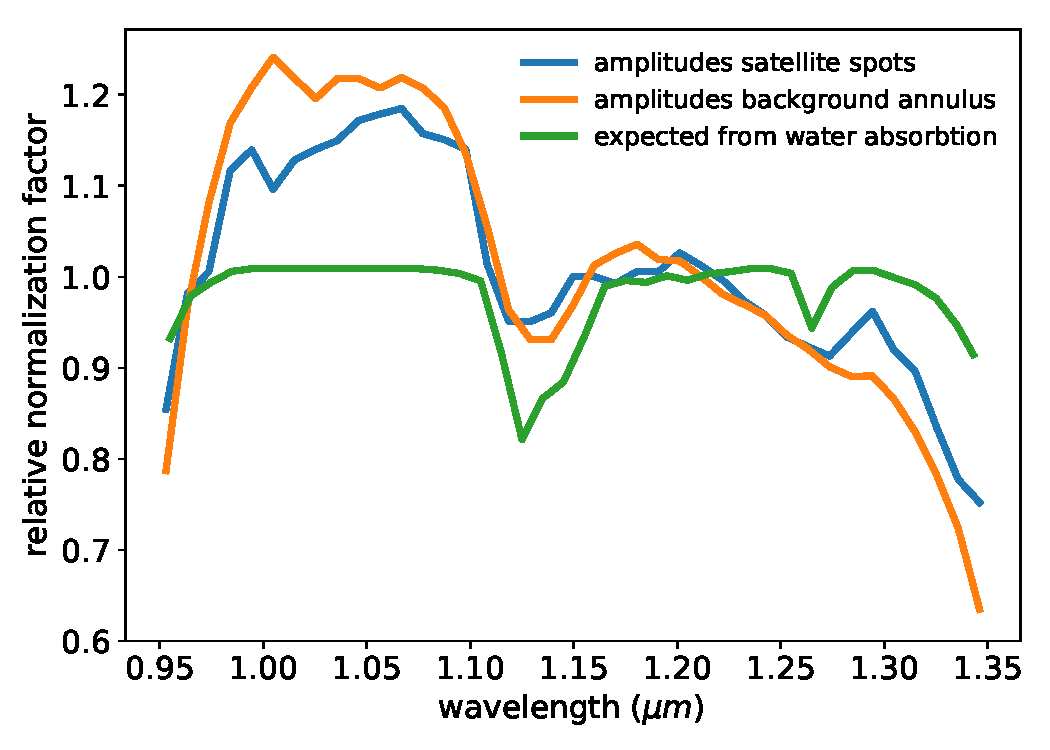
\includegraphics[width = 0.57\textwidth]{allnormalization}
\caption{The normalization factors used to normalize the data between different spectral channels. In green the expected correction due to water absorption in the atmosphere.}
\label{fig:throughputnorm}
\vspace{-5mm}
\end{wrapfigure}
The normalization factor as derived in the second way mentioned, differed slightly from the one using the center frames, especially at shorter wavelengths. This normalization left us with smaller subtraction residuals. The dips in the normalization factors line up with the expected dips in the throughput of the atmosphere due to absorbtion, since there is a big abundance of strong absorbtion lines of water in that part of the spectrum. The general trend is a decreasing flux over wavelength. The SED of the star peaks in the H band, as discussed in section 2.2 and illustrated in Figure \ref{fig:SED} \citep{Padgett2008}. This would indicate that the total incoming flux of the star should slighty increase over the range of the IFS. The fact that we see a decrease in flux instead is definitely due to wavelength dependencies in the throughput of the instrument as illustrated in Figure \ref{fig:systemthrougput}.
\bigskip

After subtracting the created model from the data, we scaled everything back to the original dimensions, so that the signal of the disk lines up in each spectral channel. The different exposures have been combined by rotating them with the corresponding field rotation, after which a median for each pixel in each spectral channel over the different exposures is taken. This provides an image with the highest SNR.

\subsection{Reference star differential imaging}
RDI is a post-processing method that uses the PSF of a reference star that is comparable to the observed star as a model to subtract the stellar PSF, but leaves the signal of the disk in the data. By the selection of a reference star, the following points have to be taken in consideration. Firstly, the throughput of the atmosphere varies over direction and time, which means that the reference star should be located close to the object of study and that the data of the reference star should be taken as close as possible to the data of the object of study, preferably during the same night. Secondly, SAXO performs better at lower R-band magnitudes, which means that the R-band magnitude of the reference star has to be from the same order as RX J1615. Thirdly, the spectral type has to the spectral type of the observed star, to be able to use its PSF as a model that can be subtracted from the reduced RX J1615 dataset. 
\bigskip

\begin{wrapfigure}{R}{0.6\textwidth}
\centering
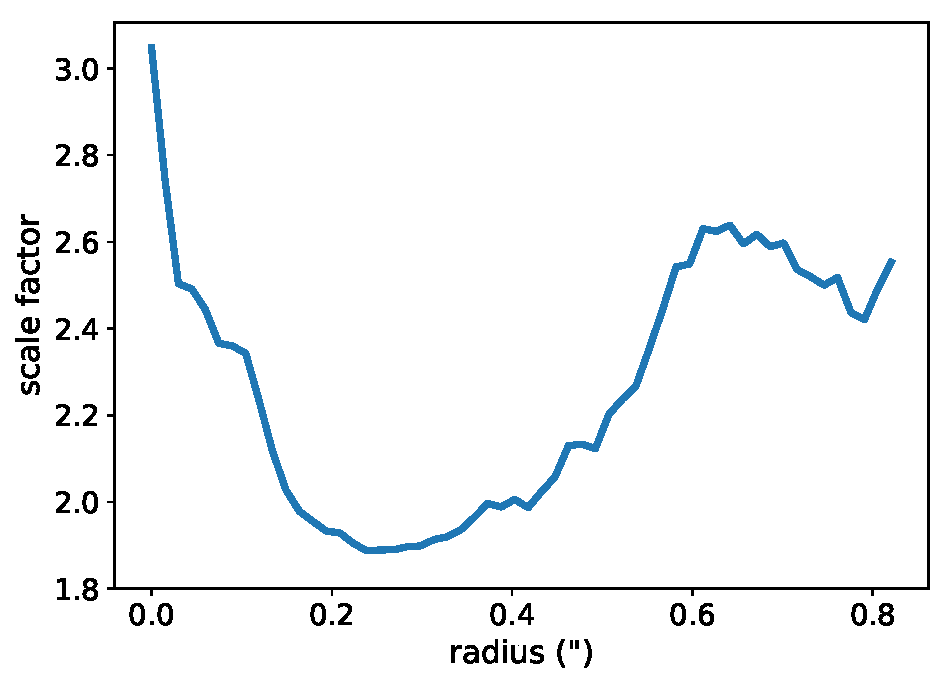
\includegraphics[width = 0.57\textwidth]{normfac}
\caption{The normalization factor against the range of the used annulus, that are used to scale the PSF of the reference star, before subtraction it from the data.}
\label{fig:rdinorm}
\vspace{-5mm}
\end{wrapfigure}

\noindent
The star TYC\_7408\_0054\_1 is used as a reference model to subtract the stellar PSF from the total signal. This star is located at 18 50 44.4873 -31 47 47.332 \cite{Gaia2016}, so close to RX J1615, has spectral type K8Ve \cite{Torres2006}, which is close to K5D, the spectral type of RX J1615 \cite{Krautter1997} and has an R-band magnitude of 10.745 \cite{Gaia2016}, which is close to 11.21, the R-band magnitude of RX J1615 \cite{Makarov2007}. Together with the fact that there is data of this star available that is taken in the same night as the RX J1615 dataset, these three parameters make this star to be a good choice for a reference star.
\bigskip

The properties of the reference star are comparable with the properties of the object, but there is still a little difference between the two PSFs. The reference star is a bit brighter than the object, which means that we have to correct for that by dividing the PSF of the reference star by a certain scale factor to reduce over subtraction. We first tried to scale the whole PSF with a scale factor, but it turned out that the PSF of the reference star differs too much from the PSF of the object, leaving both under subtracted and over subtracted parts in the image. This is probably due to a combination of the slightly different spectral type and the degrading weather conditions, which causes the PSF of the reference star to be more extended. To correct for this, the PSF of the reference star was at first spatially scaled to line up better with the stellar PSF of the object, but this did not work out good enough. Therefore, an annulus with increasing inner radius, but with a fixed width of 2 pixels is moved over both PSFs, measuring for each radius the scale factor at the part of the image where no signal is present. Only the signal of the PSF model in the corresponding annulus is then scaled with the corresponding scale factor. The change in scale factor over radius is illustrated in Figure \ref{fig:rdinorm}.

\chapter{Results of post-processing methods}
\section{ADI}
\begin{figure}[!b]
\centering 
\vspace{-0.5cm}
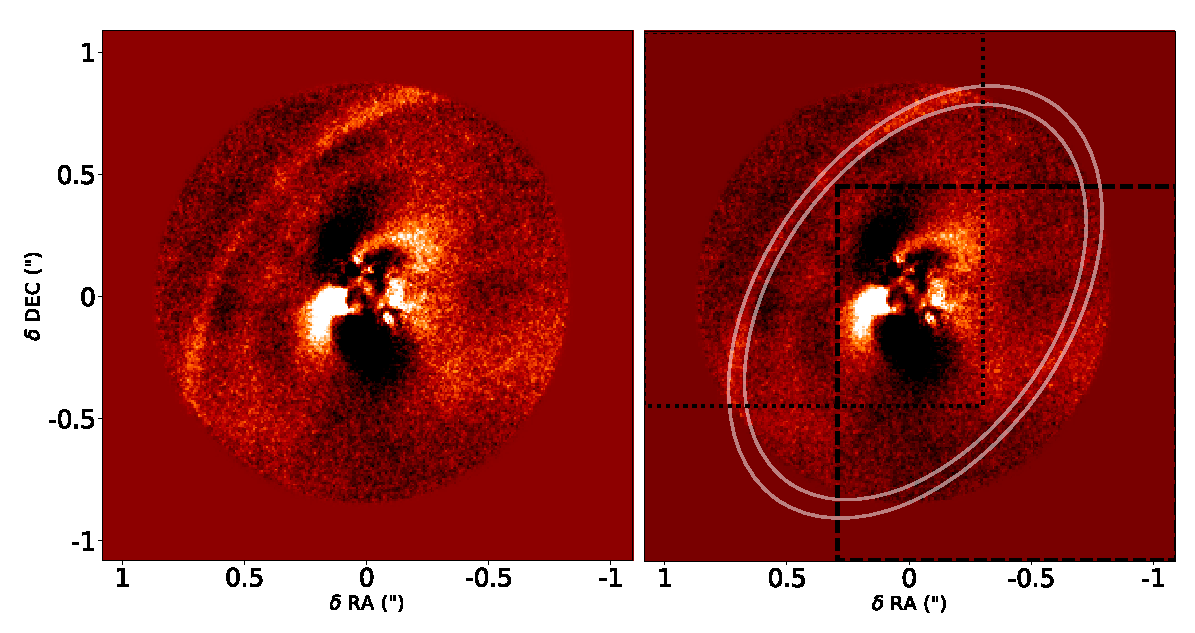
\includegraphics[trim={0cm 0cm 0cm 0cm},clip,width = \textwidth]{twoADIS}
\caption{On the left the median ADI image of all exposures over the whole Y-J wavelength range, on the right the same image together with the fitted ellipse with a semi-major axis of 0.92", semi-minor axis of 0.61" and a width of 0.067" together with the two masks that are used to select the region with the signal and the background region on the other side of the star.} 
\label{fig:aditot}
\vspace{-0.3cm}
\end{figure}

One of the rings (R2 as defined in Figure \ref{fig:irdisjos}) is well detected after the ADI reduction of the data. We determined that the ring has an elliptical shape with semi-minor axis of 0.61", semi-major axis of 0.92" and a full width half maximum of 0.067", rotated over $55^o$ as illustrated in Figure \ref{fig:aditot}. The total amount of flux of the ring in the ADI image is $437\pm 10$ counts. A similar flux calculation of the region in the fit on the other side of the star, selected with a different mask as displayed in Figure \ref{fig:aditot}, gives an estimate of the background signal of $-6\pm 9$ counts. The background signal is close to zero as expected, it being negative is a side effect of the differential imaging, due to both self-subtraction from the disk signal and oversubtraction from the flux scaling. 
\bigskip

The arc just inside this ring (A2) is visible but the signal to noise ratio of this arc is not sufficient to do any analysis on this. There are some signs for a gap between A2 and the innermost disk structures. Due to the structures of the noise in that region, it is impossible to tell the exact radius where this gap is present directly from the data. 
\bigskip

The position and shape of the disk signal in the data after the ADI reduction do not change with increasing wavelength as illustrated in Figure \ref{fig:ADIcolor}. As visible in Figure \ref{fig:aditot}, the ring gets fainter when it approaches the minor axis of the fitted ellipse. This is due to selfsubtraction of the ring in the ADI routine, since the ring approaches a circular shape at that point as seen from the center of rotation. The total signal of the disk does increase towards longer wavelenghts. The shape of the ring and the variations in flux, however, do not change with wavelength. The large scale structures in the background do not change as well between the different wavelength bins.

\begin{figure}[htb]
\centering
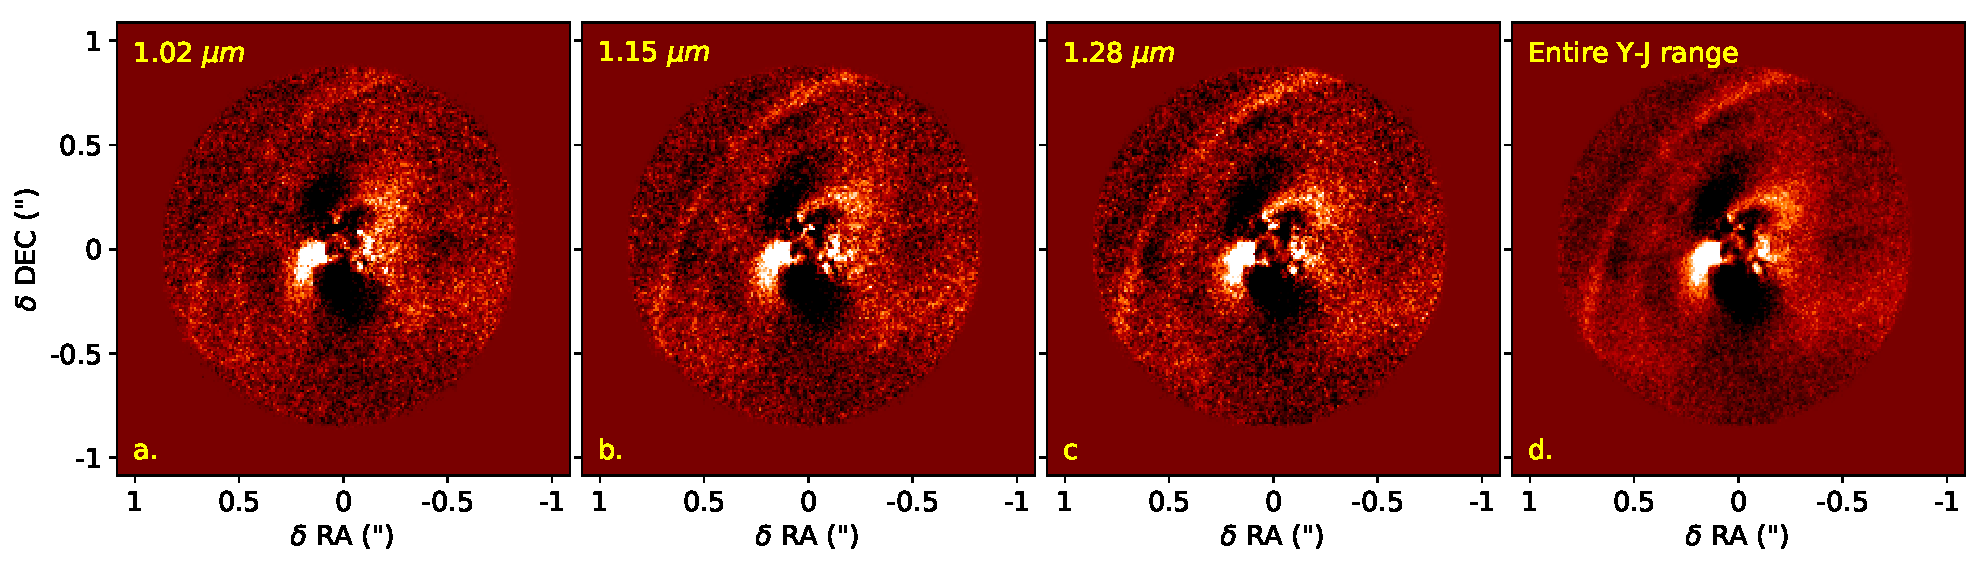
\includegraphics[trim={0cm 0cm 0cm 0cm},clip,width = \textwidth]{ADIwavelplot}
\caption{Reduction of IFS ADI data. From left to right: \textbf{a:} median of 13 channels (0.96-1.07$\mu m$) \textbf{b:} median of 13 channels (1.08-1.21 $\mu m$) \textbf{c:} median of 13 channels (1.22-1.33 $\mu m$) \textbf{d:} median of the entire YJ range}
\label{fig:ADIcolor}
\end{figure}

\clearpage
\section{SDI}
\begin{wrapfigure}{R}{0.5\textwidth}
\vspace{-0.5 cm}
\centering
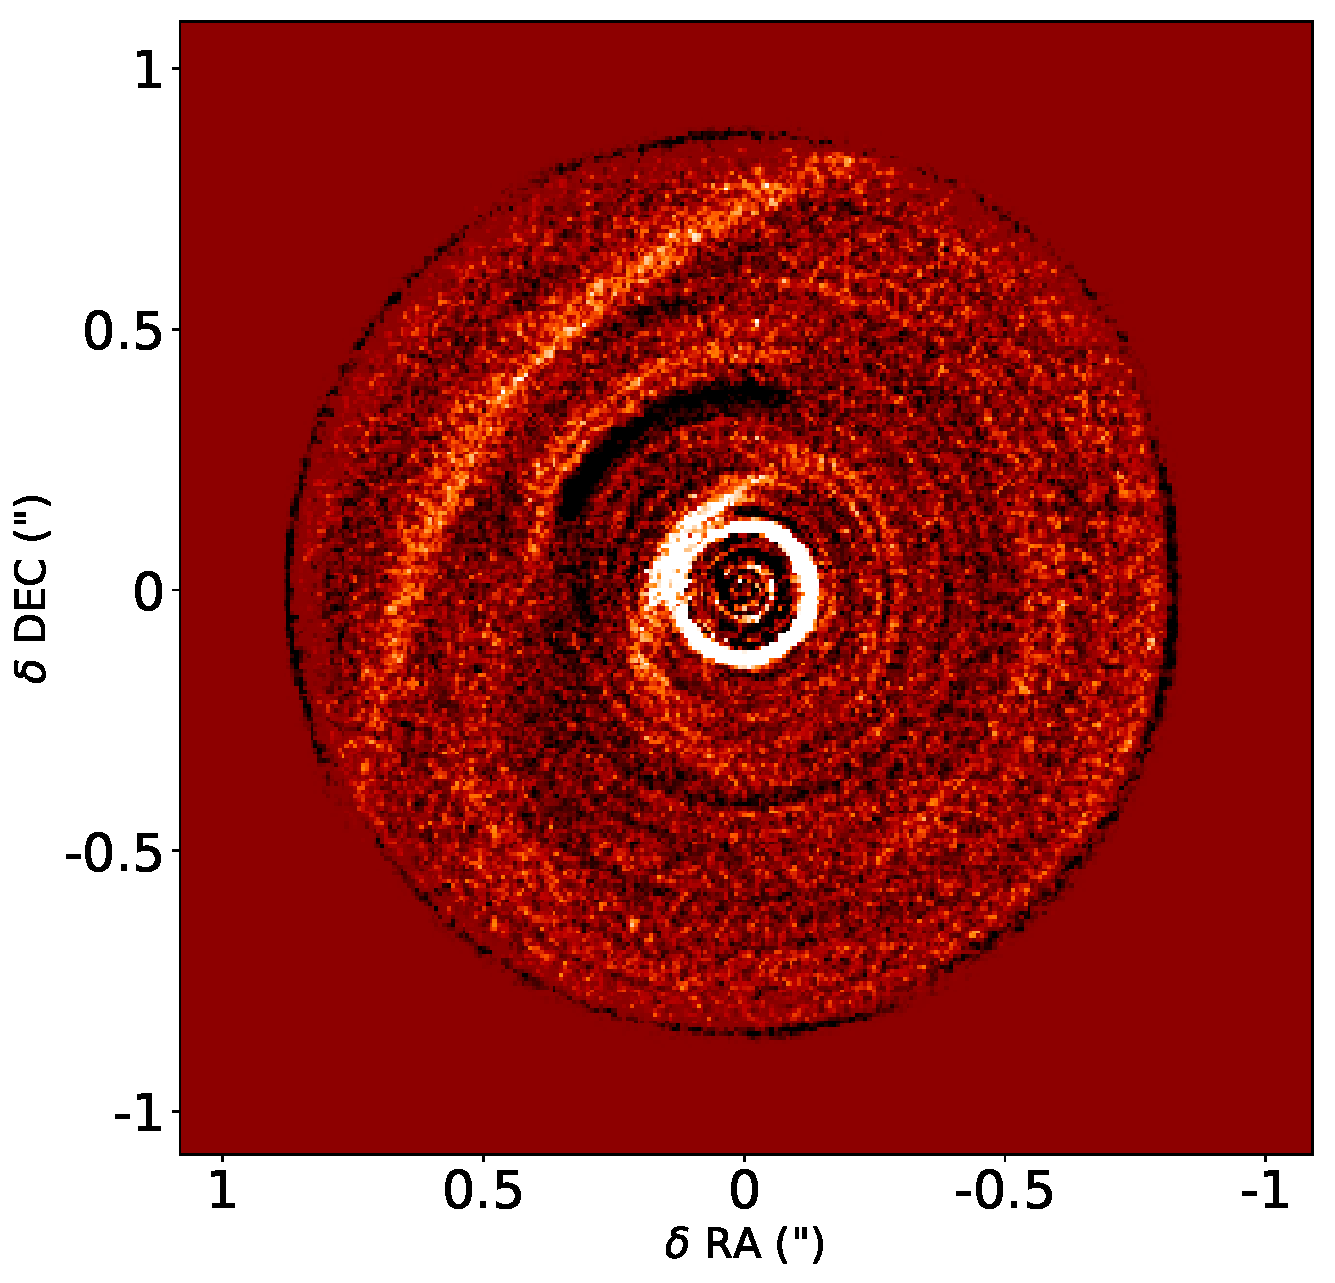
\includegraphics[width=\linewidth]{SDI_tot}
\caption{The median SDI image of all exposures over the whole Y-J wavelength range of RX J1615}
\label{fig:SDI_tot}
\vspace{-0.7 cm}
\end{wrapfigure}

The outermost ring segment (R2) that is visible after the ADI reduction is also visible after the SDI reduction. By using the same aperture as in the analysis of the ADI image, we measured the total flux of the ring after applying SDI on the data to be 644 $\pm 13$ counts. This is a bit more than the total flux of the ring after applying ADI. The flux in the background, measured in the same aperture over the same area on the other side of the star, is 73 $\pm 11$ counts. This is also more than after applying ADI, leaving slightly more signal of the disk in the SDI image after subtraction of the total flux of the background.  
\bigskip

A2, the arc just inside R2, is visible as well, but its shape has changed with respect to the ADI reduction. This is probably due to the dark region just inside A2, which is caused by a bad spot on the detector, that ends up as an arc in the data due to the field rotation between the different exposures. This bad region could distort the model for the PSF of the star after scaling the whole image according to its wavelength, as mentioned in chapter 4. The bad region is then smeared out over a larger region of the image, leaving some negative signal in that region for certain wavelengths before taking the median to build a model for the stellar PSF. This could cause A2 to be more prominent above the bad region and look much more circular than after applying ADI. 
\bigskip

The innermost disk structure (I1) is much more prominent in the SDI data than in the ADI data. It is clearly visible that this has a ringlike shape over a range of almost $180^o$. The closed circular ring at an angular separation of 0.15" is an artefact of the reduction method, probably due to the structure in the raw signal that is caused by the coronagraph, as displayed in Figure \ref{fig:reduceddata}. Furthermore, the SDI image does show much less large scale structures in the background than the ADI image. This could either mean that these structures are created during the ADI procedure, but cancelled more efficiently in the SDI data, or that this is astrophysical data which is picked up in the ADI data, rather not in the SDI data.
\bigskip

From Figure \ref{fig:SDIcolor} it becomes clear that the signal of the disk increases with increasing wavelength, just as the signal after applying ADI does. The disk signal being positive at longer wavelengths and negative at shorter wavelengths is an artefact of the classical SDI routine. {\parfillskip0pt\par}

\begin{figure}[htb]
\centering
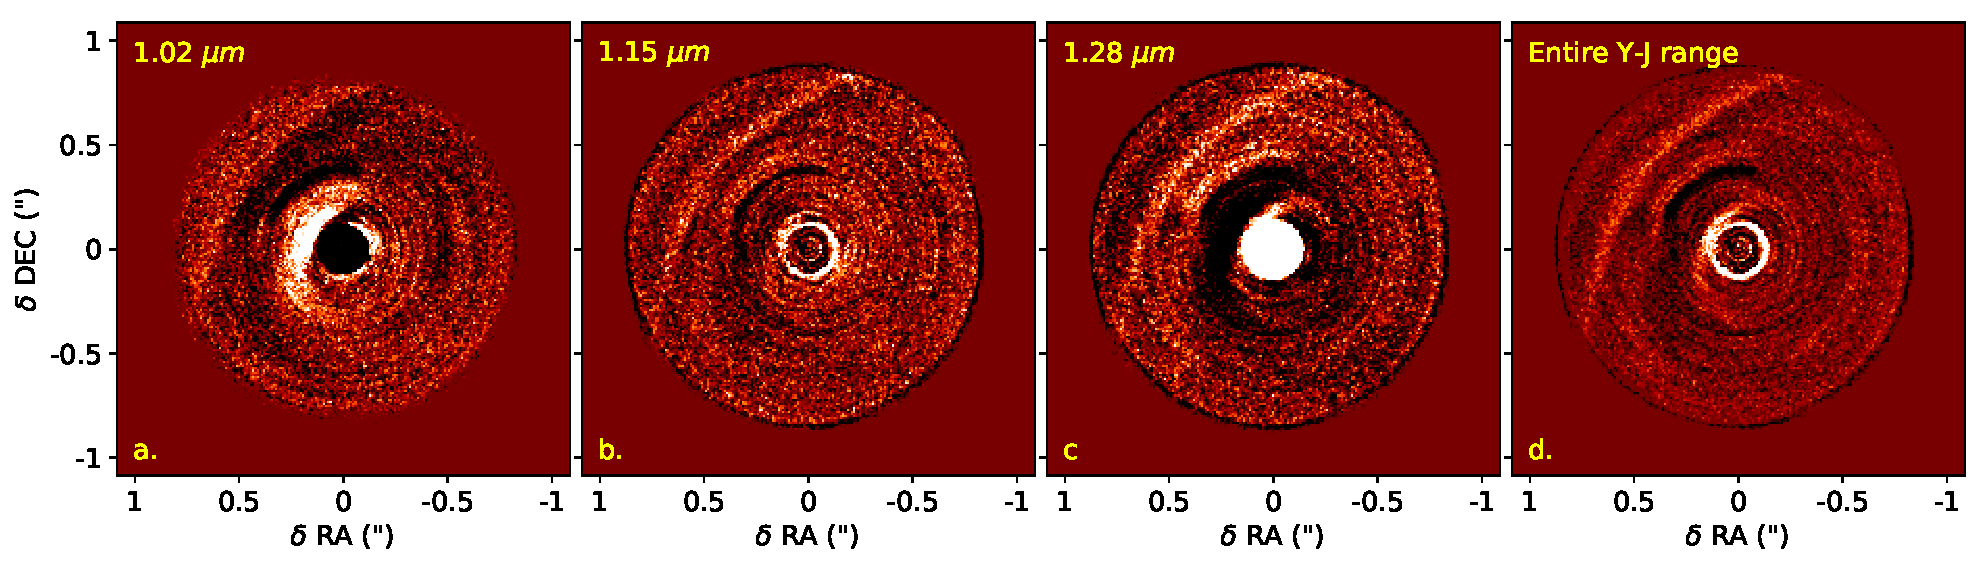
\includegraphics[trim={0cm 0cm 0cm 0cm},clip,width = \textwidth]{SDIwavelplot}
\caption{Reduction of IFS SDI data. From left to right: \textbf{a:} median of the first 13 channels (0.96-1.07$\mu m$) \textbf{b:} median of 13 channels (1.08-1.21 $\mu m$) \textbf{c:} median of 13 channels (1.22-1.33 $\mu m$) \textbf{d:} median of the entire YJ range}
\label{fig:SDIcolor}
\end{figure}

\noindent
Taking just the median over wavelength per pixel leaves some signal of the disk in the model of the PSF, causing some areas to be over-subtracted and other areas to be under-subtracted. This changes over wavelength since the signal of the disk in the model for the PSF in the SDI routine is rescaled corresponding to the wavelength.
\clearpage

\section{RDI}
\begin{wrapfigure}{R}{0.5\textwidth}
\vspace{-6mm}
\centering
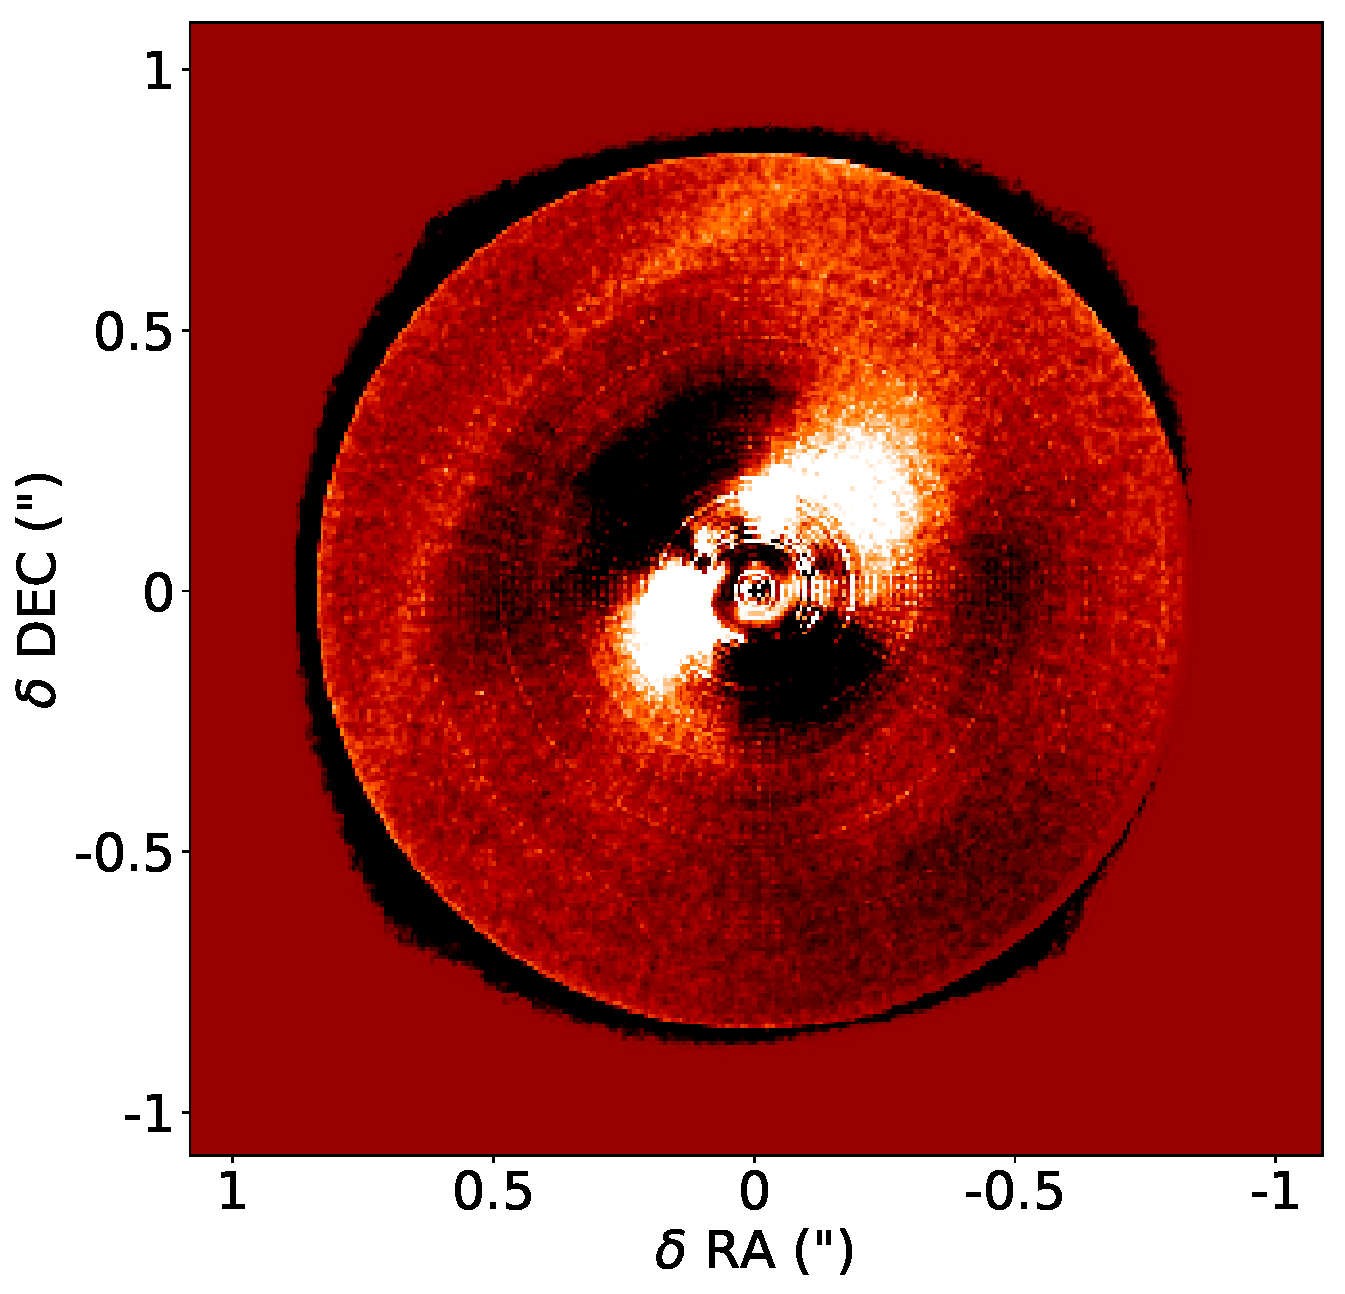
\includegraphics[width=\linewidth]{RDI_tot_smallimcon}
\caption{The median RDI image of all exposures over the whole Y-J wavelength range of RX J1615}
\label{fig:RDI_tot}
\vspace{-4mm}
\end{wrapfigure}

R2 is detected in the RDI image as well, as illustrated in Figure \ref{fig:RDI_tot} and has a total flux of $915 \pm 56$ counts and a total flux in the background of $-599 \pm 40$ counts. This is much more than the flux in the ADI and SDI image, probably because ADI and SDI have to deal with a lot of self-subtraction. RDI is a much more reliable measure for the total disk brightness. A2 is not recovered in the RDI image, since the parts closest to the center are affected the most by small differences between the two PSFs. Additionally, A2 is  already hardly visible in the ADI and SDI image. It is noticeable that the PSFs were not exactly the same, since we have unexpected darker regions and negative values in the final image.
\bigskip

The variations in the disk surface brightness over wavelength are illustrated in Figure \ref{fig:RDIcolor}, where the data is median combined in three wavelength bins. These images have the same color scale as the ADI and SDI images, for a good comparison. The signal of the disk is already well recovered at shorter wavelength and increases to longer wavelengths, just as we expected from the ADI and SDI reduction.

\begin{figure}[htb]
\centering
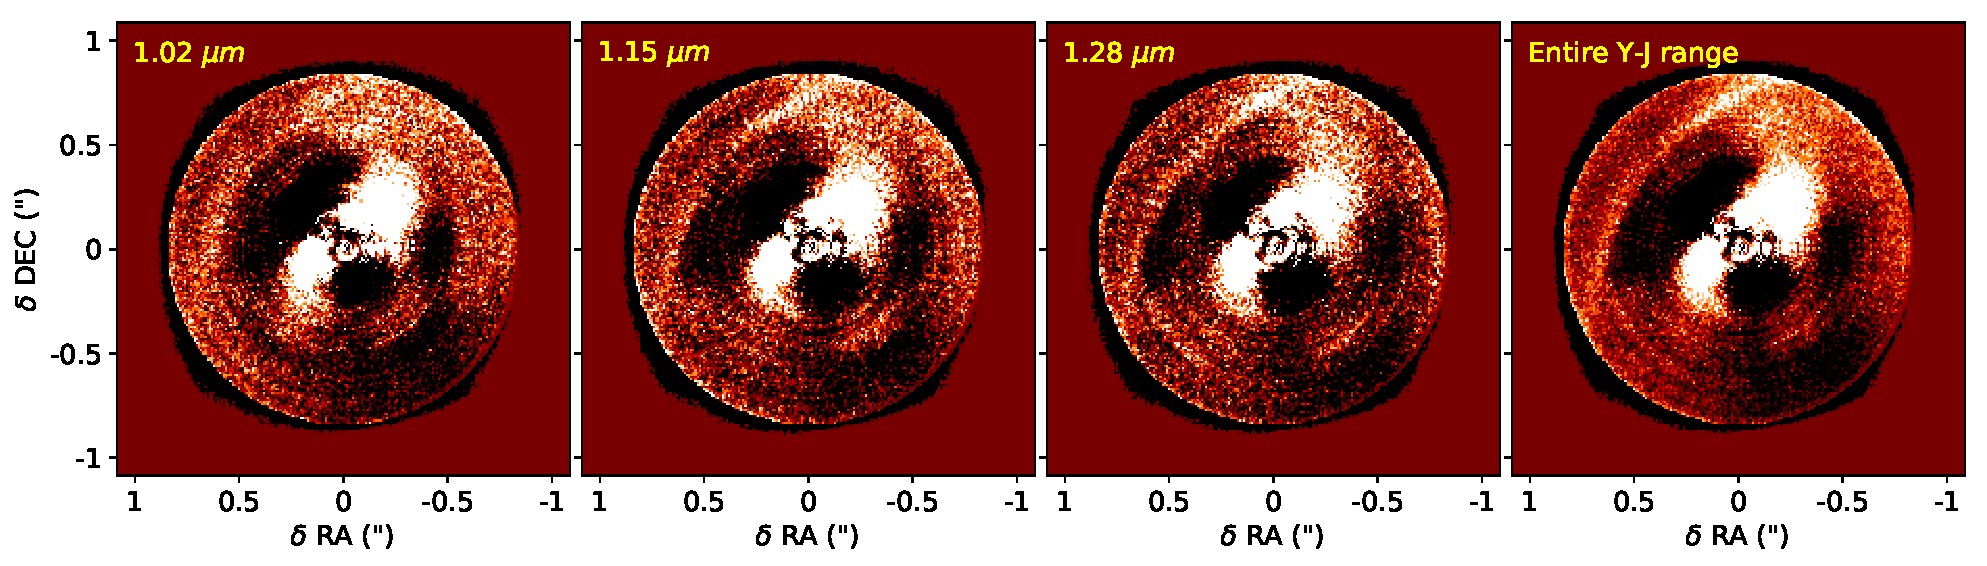
\includegraphics[trim={0cm 0cm 0cm 0cm},clip,width = \textwidth]{RDI_color_imcon}
\caption{Reduction of IFS RDI data. From left to right: \textbf{a:} median of 13 channels (0.96-1.07$\mu m$) \textbf{b:} median of 13 channels (1.08-1.21 $\mu m$) \textbf{c:} median of 13 channels (1.22-1.33 $\mu m$) \textbf{d:} median of the entire YJ range}
\label{fig:RDIcolor}
\end{figure}

\chapter{Spectral analysis}
\section{Morphology changes in the disk}

The resulting morphology of the disk in the data is different, depending on the post-processing techniques that are used. In the ADI image, illustrated in \ref{fig:aditot}, there is a clear dip in the signal visible at the point where the ring approaches the minor axis of the fitted ellipse. To quantify this change in flux throughout the ring, we measured the flux in a circular aperture with a radius of 0.067", the FWHM of the ring, and dragged it over the whole ring. This analysis is shown in Figure \ref{fig:coloroverangle}. This figure illustrates that the ring in the ADI image approaches zero at an azimuthal angle of about $50^o$ in the different wavelength bins. The signal in the SDI image is much more constant throughout the ring. 
\bigskip

The measurement error on the analysis is in the order of 2 counts, but the total error is dominated by the effects of the post-processing procedure. This is very hard to determine, which is the reason that we did not give an error on the determined flux. Since the total effective flux of R2 in the SDI image is a bit higher than in the ADI image, we can conclude that part of the signal in the ADI image is selfsubtracted. This is due to the fact that the ring approaches a circular shape, which means that it shows up on the same location in each exposure. The model for the stellar PSF contains hence part of the signal in that region, which means that the disk signal is subtracted from the image. 
\bigskip

The flux of the signal in the RDI reduction has also a clear dip at about the same azimuthal angle. This is probably caused by morphology differences between the stellar PSF of the object and the PSF of the reference star, which affects the end result more closer to the center of the image. The PSF created in the SPHERE instrument is very stable over time, thanks to the extreme adaptive optics, but does change still due to changing conditions in the atmosphere.
\bigskip

\begin{figure}[!t]
\centering
\vspace{-0.3cm}
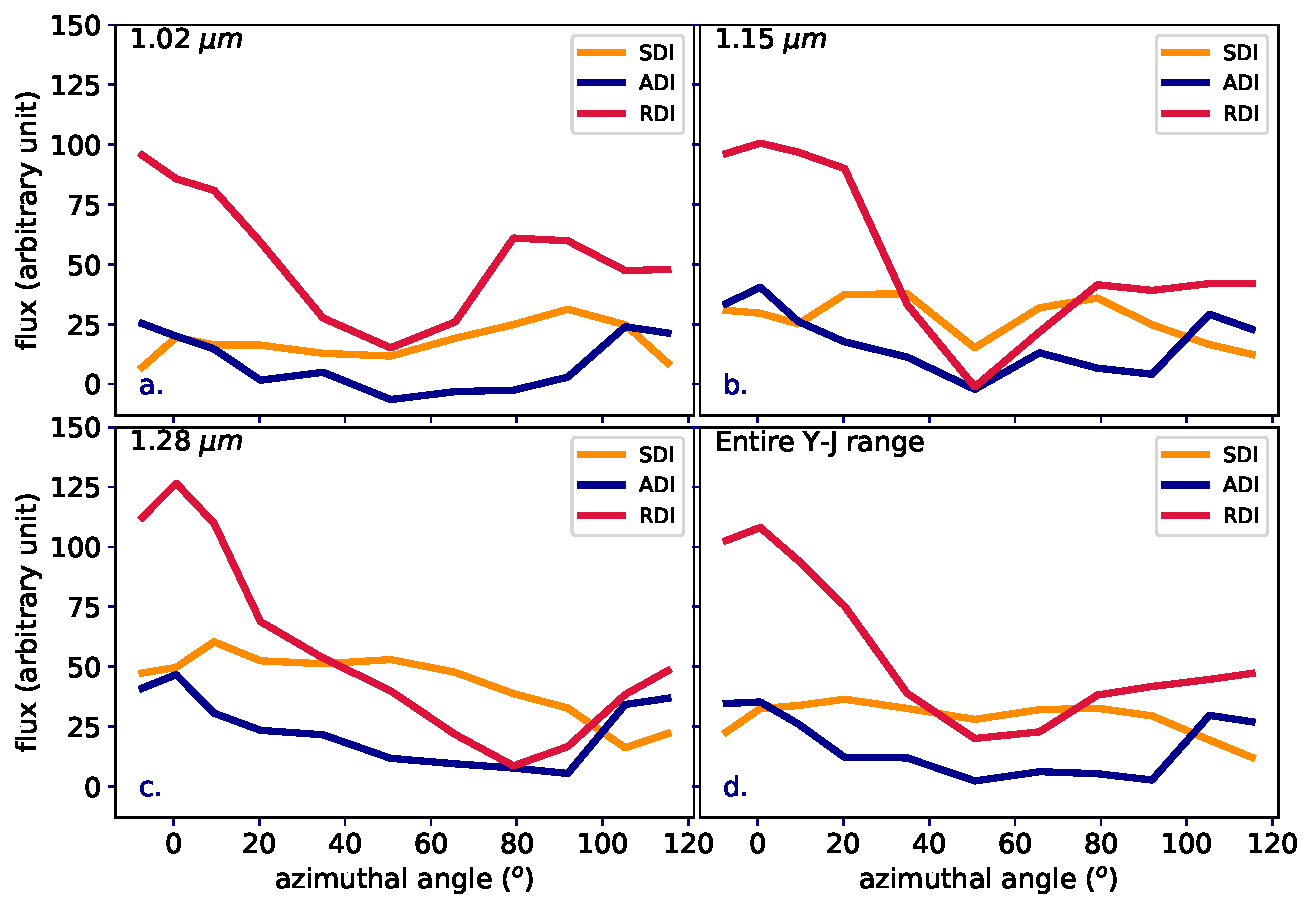
\includegraphics[trim={0cm 0cm 0cm 0cm},clip,width = 0.9\textwidth]{coloroverazimangle}
\caption{The relative flux over azimuthal angle in three different wavelength bins \textbf{a:} 13 channels (0.96-1.07 $\mu m$) \textbf{b:} 13 channels (1.08-1.21 $\mu m$) \textbf{c:} 13 channels (1.22-1.33 $\mu m$) \textbf{d:} signal of the whole spectrum}
\label{fig:coloroverangle}
\vspace{-0.5cm}
\end{figure}

The innermost disk structure is much better recovered in the SDI image. On small radii from the center of rotation, the signal has not moved enough over the detector if the field rotates with $4^o$ per exposure to do ADI, which means that the signal is distorted. Since this structure is not that large, it does not show up too much in the model in the SDI prodecedure, which means that it looks cleaner in the final SDI image.
\bigskip

\section{Brightness changes throughout disk}
As already visible in Figure \ref{fig:coloroverangle} and worked out further in Figure \ref{fig:coloroverpos}, where the amount of disk signal is plotted against wavelength in the three different regions as defined in Figure \ref{fig:regions}, the amount of signal does change over wavelength. A linear trend is visible in all three reductions. The signal in the SDI image fluctuates much over wavelength in region 1, {\parfillskip0pt\par}

\begin{figure}[!t]
\centering
\vspace{-0.3cm}
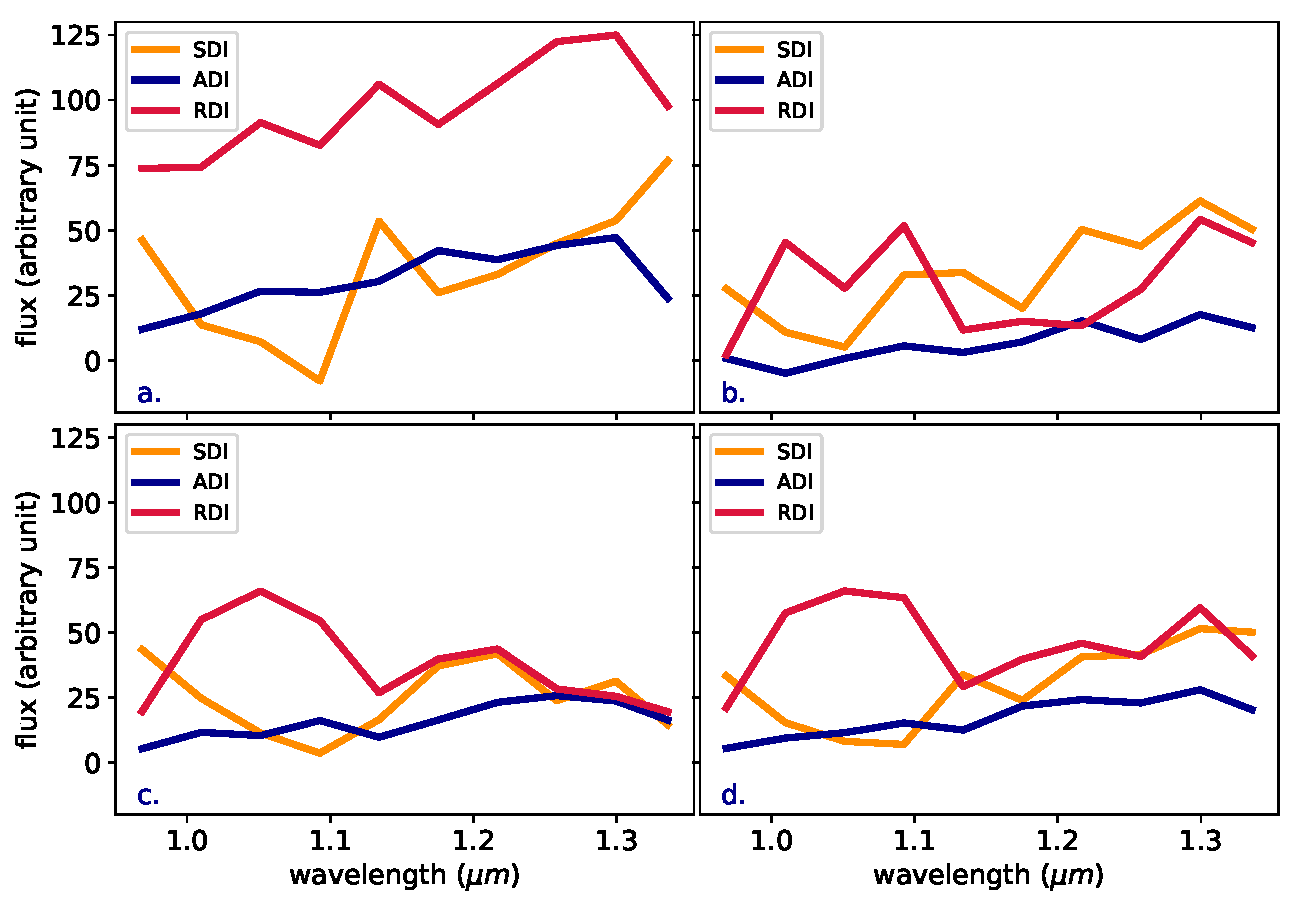
\includegraphics[trim={0cm 0cm 0cm 0cm},clip,width = 0.9\textwidth]{colorregions}
\caption{The relative flux of the signal over wavelength in the three regions as defined in Figure \ref{fig:regions} and in the whole ring: \textbf{a:} region 1 \textbf{b:} region 2 \textbf{c:} region 3 \textbf{d:} signal of the whole ring.}
\label{fig:coloroverpos}
\vspace{-0.5cm}
\end{figure}

\begin{wrapfigure}{R}{0.5\textwidth}
\vspace{-0mm}
\centering
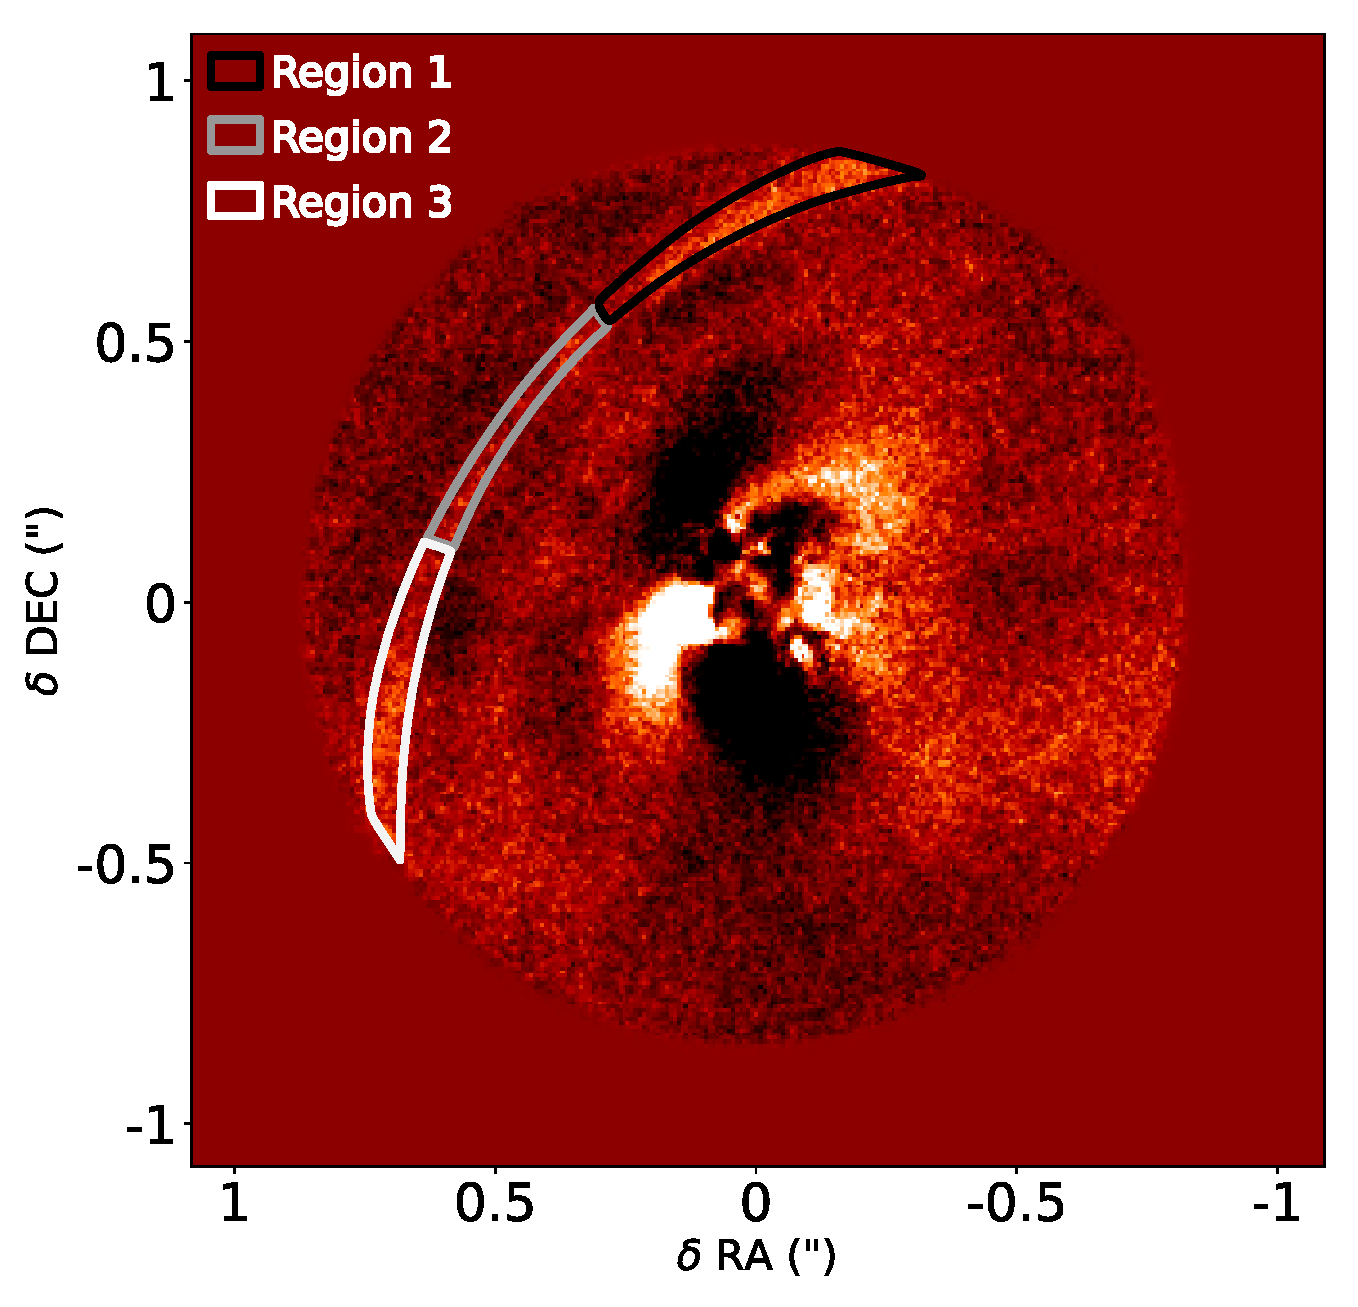
\includegraphics[width=1\linewidth]{ADIregions}
\caption{The ADI image over the whole YJ range, with the three marked regions between respectively -$10^o$ and $30^o$ for region 1, $30^o$ and $70^o$ for region 2 and $70^o$ and $110^o$ for region 3, that are used to compare the local features in the ring}
\label{fig:regions}
\vspace{-9mm}
\end{wrapfigure}

\noindent
which probably is because of edge effects and the unexpected negative values at shorter wavelengths, as shown in Figure \ref{fig:SDIcolor}. The RDI data shows multiple times a peculiar bump at short wavelengths. This is probably because of degrading weather condition during the aquiring of reference star data, which makes the shape of the PSF of the reference star less stable. Since shorter wavelengths have a lower Strehl ratio, the degrading weather condition will affect the end result more at the lower end of the spectrum.
\bigskip

It is unclear whether or not we could trust this wavelength dependence of the disk brightness. The guide star is faint (R = 11.21 mag) \citep{Makarov2007}, which means that the Strehl ratio in the R-band was very poor ($SR_R < 3$\%\citep{DeBoer2016}). A poor Strehl ratio means that the performance of SAXO is not optimal, meaning that structures can be smoothed out. Since the performance of SAXO gets better for longer wavelengths and signal is present close to R2, it is impossible to say if the increase in brightness over wavelength is partly astrophysical or just an increased SAXO performance. Some signal could be washed out of the disk signal due to the low resolution. If the wavelength dependence is astrophysical, it could be caused by variations in the grain size or the chemistry throughout the disk. %{\parfillskip0pt\par}
\bigskip

\begin{wrapfigure}{R}{0.6\textwidth}
\vspace{-6mm}
\centering
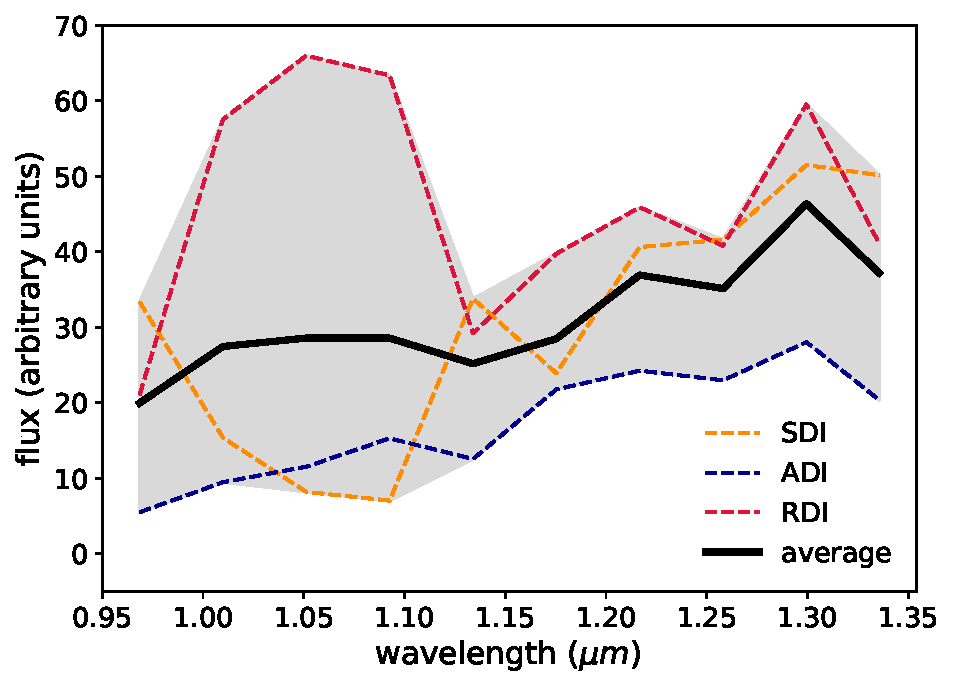
\includegraphics[width=1\linewidth]{totflux}
\caption{The expected disk brightness over wavelength, together with the results after applying the different post-processing methods, which gives a measure for the error.}
\label{fig:totflux}
\vspace{-4mm}
\end{wrapfigure}

%\noindent
A better analysis of A2 and the innermost disk component could indicate if this change in surface brightness is astrophysical, since the surface brightness of these structures should change as well if the mechanism behind this is the increase in performance of SAXO at longer wavelengths. Radiative transfer models could be used as well to find an answer whether we are looking at a true astrophysical change in surface brightness with increasing wavelength or a result of the bad Strehl ratio, but that is beyond the scope of this project.
\bigskip

Calculating the exact error on the data points is difficult, since it is hard to determine how much of the signal is smoothed out due to the poor Strehl ratio and how much self-subtraction is going on during the different procedures. This is why error bars are not included in the figures. We know that all the data comes from the same dataset, which means that the signal of the disk is always the same no matter what reduction method is used. The error on the astrophysical brightness over wavelength is hence at least as much as the difference between the different reduction methods, as illustrated in Figure \ref{fig:totflux}. As gets clear in this image, the disk in the RDI image seems much more blue than in the ADI and SDI image. This is probably due to the degrading weather conditions during the reference star run, meaning that the PSF is less comparable with the stellar PSF of the object. This change is much more drastic in shorter wavelength, since the Strehl ratio is worse at lower wavelength, which means that the disk signal there is locally stronger contaminated with residual stellar signal which makes it appear to be blue.
\bigskip

\begin{wrapfigure}{R}{0.6\textwidth}
\vspace{-6mm}
\centering
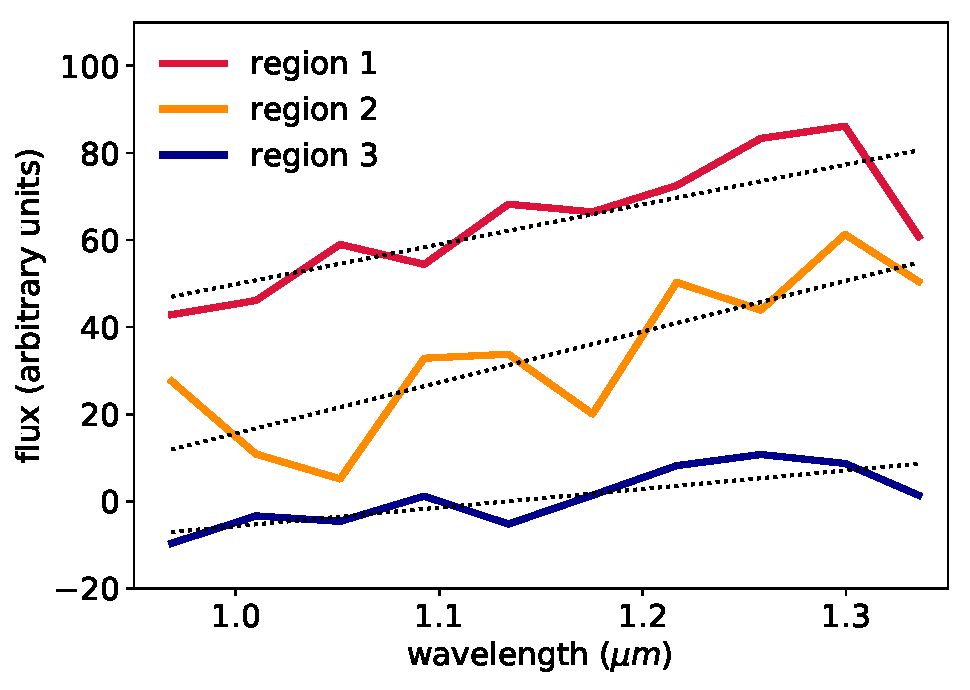
\includegraphics[width=1\linewidth]{slopedifreg}
\caption{The relative flux of the signal over wavelength which we can trust in the three regions with respectively an azimuthal angle between $-10^o$ and $30^o$ for region 1, between $30^o$ and $70^o$ for region 2 and between $70^o$ and $110^o$ for region 3. There is an arbitrary offset between the different slopes for a better illustration.}
\label{fig:slopedifreg}
\vspace{-4mm}
\end{wrapfigure}
A difference in the color in different regions of the outermost ring could be a sign that the grain properties are not the same in the whole disk. To measure the exact slope of the increase in surface brightness over wavelength throughout the ring, which is an indication of the color, we should discard the data that suffers from over subtraction and self-subtraction and use only the data that we can trust in the different regions. As mentioned earlier, the ADI image has much self-subtraction where the ring approaches the minor axis and the RDI image has more over subtraction close to the center where small differences between the PSF of the reference star and the object affect the end results much more drastically. In the SDI procedure however, the signal moves perpendicular to the ring on the minor axis by scaling the image, meaning that the SDI result has the least amount of self-subtraction in this region. This means that we can trust the SDI image the best in region 2. SDI has to deal with more self-subtraction on the edges and is plagued by edge effects due to the fact that after scaling the images, the edges have significantly less data, which gives a lower SNR in the resulting image. This means that we could better discard the SDI data out of the analysis of region 1 and region 3. The RDI data does behave different in region 3 than both the other regions and the ADI and SDI data, probably due to a combination of a lower SNR ratio in that region in all the data and the degrading weather conditions during the aquiring of the reference star data, which affects short wavelengths significantly more.
\bigskip

As illustrated in Figure \ref{fig:slopedifreg}, the slope of flux against wavelength is comparable in region 1 and 2. The brightness changes much less over wavelength in region 3, which could be due to the lower SNR in all the data in that region.

\chapter{Additional research}
\begin{wrapfigure}{R}{0.6\textwidth}
\vspace{-6mm}
\centering
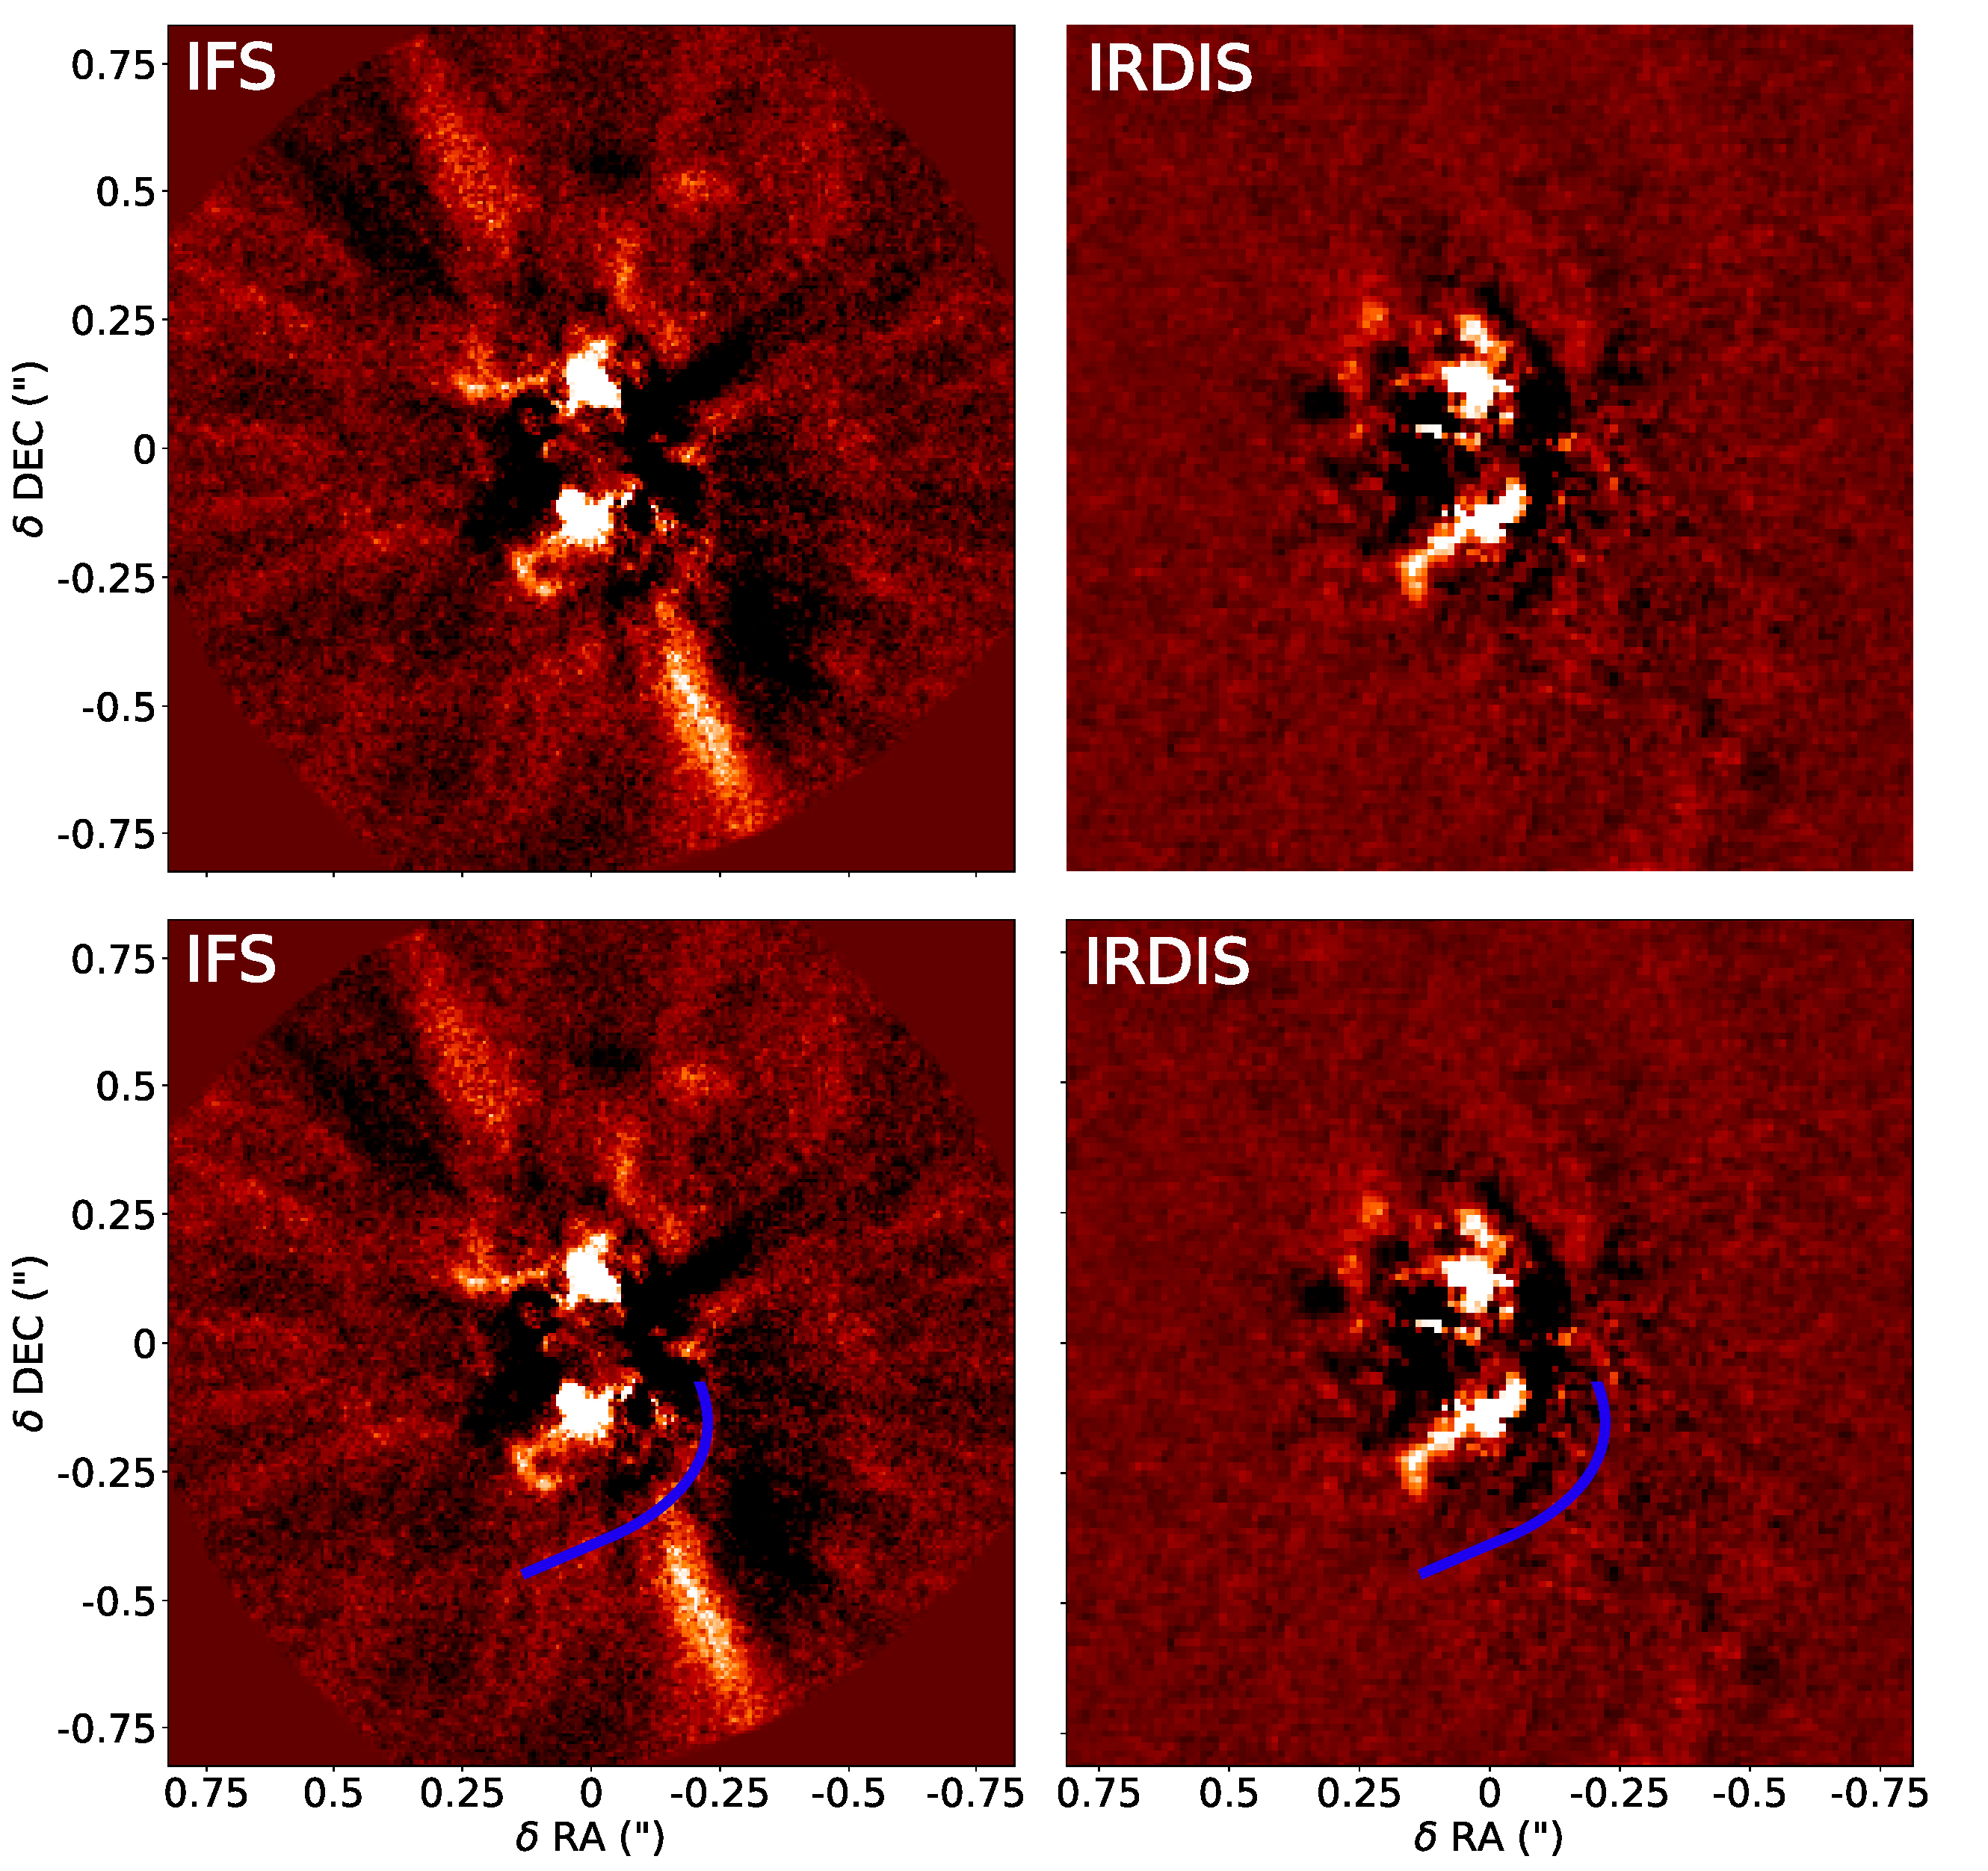
\includegraphics[width=\linewidth]{hdadi}
\caption{ADI image of IFS data on the left and IRDIS data on the right. A spiral arm launching in the west and extending towards the south is highlighted in both image on the figures at the bottom}
\label{fig:hdadi}
\vspace{-8mm}
\end{wrapfigure}

After we got good results on the dataset of RXJ1615, we ran the same program over a dataset of HD97048. HD97048 is a Herbig Ae star, which means that it is a young intermediate mass star. It harbors a well known transition disk that has been previously resolved by \citep{Ginski2016} with SPHERE IRDIS. The disk is highly structured showing multiple rings out to ~340. The rings of this object that were best visible in IRDIS data are mostly located outside the FOV of the IFS, but the IFS classical ADI reduction appears to have higher signal-to-noise in the detected disk structures, as illustrated in Figure \ref{fig:hdadi}.
\bigskip

In the IFS classical ADI reduction, the inner disk looks very similar to the polarimetric IRDIS image in \citep{Ginski2016}, which has basically no self subtraction, which means that we can trust the morphology of the disk in the IFS ADI reduction. In the IFS data, an additional feature is noticeable, that is not described in the initial paper. A spiral arm is visible, launching in the west and extending toward the south, as highlighted in Figure \ref{fig:hdadi}. This spiral arm could be a sign of ongoing planet formation in the disk, since the spiral arm is probably created by interactions between the inner disk and a planet.
\bigskip

One of the reasons why this feature is better visible in IFS data than in IRDIS data could be that IFS uses a broader wavelength range than IRDIS, since this data was taken in the narrow H band filter, so the IFS may overall have received more light. Another reason could be that the scattering efficiency of the grains in the spiral arm is higher at shorter wavelength, which are included in IFS data, but not in IRDIS data. This could also be the reason that the inner disk also seems to be stronger in the IFS data than in IRDIS. It is also possible that the centering routine was better than the standard recipe from the ESO pipeline, which is used to center the IRDIS data, since for a tenuous structure like this, centering is very important. 
\bigskip

A next step that could be taken in the research on this object is the use of a more advanced ADI algorithm such as PCA or T-LOCI to increase the SNR of the spiral arm. Additionally a proposal for follow up observations of this disk has been submitted earlier this year, which should be sensitive to this feature. With a better resolved spiral arm, it could be possible to determine the mass of the planet that is disturbing the inner disk.

\chapter{Discussion}
\section{Comparing classical ADI with TLOCI}
\begin{figure}[!b]
\centering
\vspace{-0.3cm}
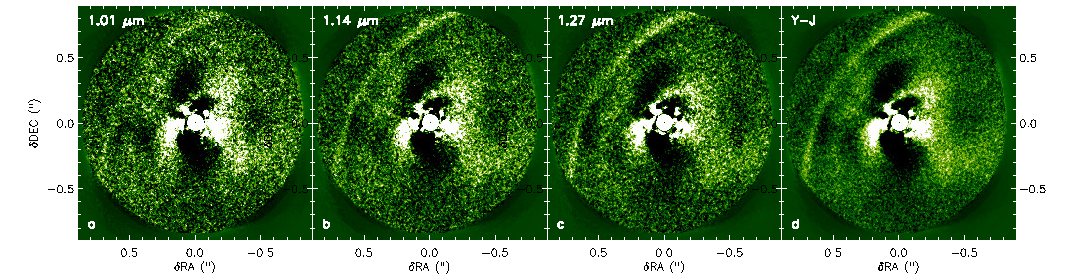
\includegraphics[trim={0.3cm 0cm 1.2cm 0cm},clip,width = .985\textwidth]{ifsjos}
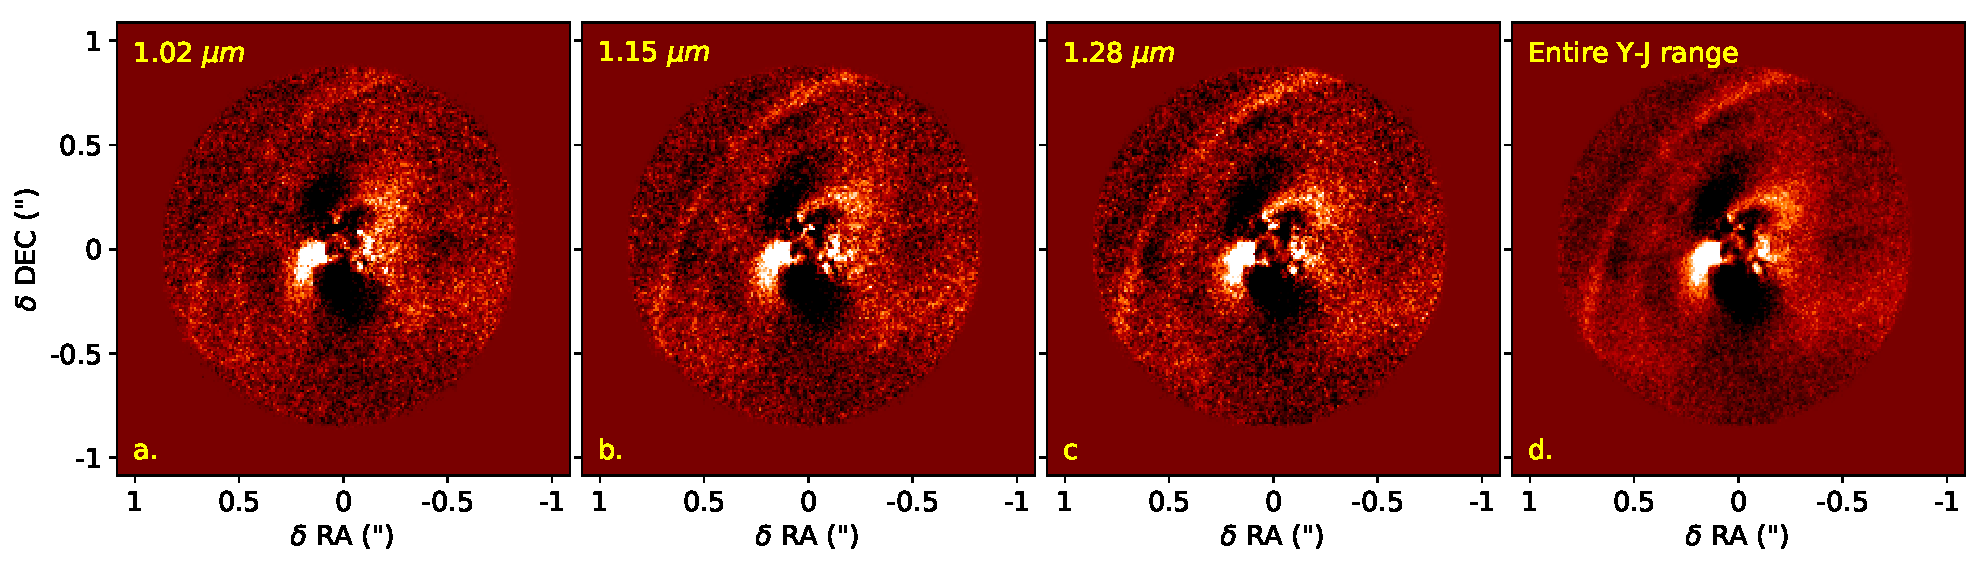
\includegraphics[trim={0cm 0cm 0cm 0cm},clip,width = \textwidth]{ADIwavelplot}
\caption{From top to bottom: the T-LOCI ADI reduction and the classical ADI reduction. From left to right: \textbf{a:} median of 13 channels (0.96-1.07$\mu m$) \textbf{b:} median of 13 channels (1.08-1.21 $\mu m$) \textbf{c:} median of 13 channels (1.22-1.33 $\mu m$) \textbf{d:} median of the entire YJ range}
\label{fig:coloroverpos}
\vspace{-0.5cm}
\end{figure}

A comparison between the reduced image of the classical ADI as done during this research and the T-LOCI ADI reduction provided in earlier research does not show big differences. The morphology of the clear resolved ring and the structures in the background are the same in both images and by vizual inspection the signal-to-noise ratio in the classical ADI images look compareable or better than in the original T-LOCI reduction. This means that the median of the different exposures, as created during the ADI procedure, is already a good reference for the stellar PSF and does not contain much disk signal. The reason why the more advanced reduction method T-LOCI does not make the signal of the disk better detectable in this case is probably the amount of field rotation in the dataset. With $69^o$ over 16 exposures, is this very good, meaning that there is a minimum amount of self subtraction going on in the dataset. This makes the classical method used a pretty good model for the stellar PSF, taking all the excess signal out of the data, but leaving as much signal of the disk as possible in the final image. Since T-LOCI is a more agressive subtraction algorithm than classical ADI, it may well be possible that the algorithm subtracted actually more disk signal when it tried to fit the stellar PSF. 

\section{Further research}
There are several steps that are possible to take after this project. One step could be the error propagation in the different procedures. The estimation on the error of the astrophysical flux is now very rough, but a good approximation of the error bars could improve the conclusions we have now. The results we have can not be interpreted more than a general trend, due to the missing errorbars.
\bigskip

The use of more advanced post-processing algorithms, such as Principal Component Analysis (PCA), could be a good next step, since this may reduce the amount of selfsubtraction in the different images. PCA constructs a database of eigenimages of PSFs and from that database constructs a much better model for the stellar PSF, decreasing the amount of self-subtraction in the routines. More advance methods should also solve the issue in the SDI data that the signal is negative at shorter wavelengths, since more advanced methods should leave more disk signal out of the model of the stellar PSF.

\chapter{Conclusion}
We can conclude that the basic reduction works well with the common pipeline of ESO. Esoreflex provides a user-friendly and flexible way to run the different recipes of the pipeline, which gives high-quality results in the end. The data of the IFS is a bit noisy in the small scale FOV, but classical post-processing methods are still able to recover most of the disk signal from the data.
\bigskip

We can conclude that the post-processing methods have an effect on the morphology of the disk. The brightness of R2 in the ADI image dips around the minor axis of the fitted ellipse due to self-subtraction, since the disk approaches a circular annulus at that point. In the ADI image, there are more structures resolved in the background than in the SDI image, but the innermost structures are better resolved in the SDI image due to selfsubtraction in the ADI image.
\bigskip

The surface brightness increases to longer wavelengths, but we do not have enough evidence to say whether or not this is an astrophysical property or just a result of the increasing Strehl ratio to longer wavelengths. The increase in surface brightness is comparable throughout the outermost ring that we studied, which means that we have not enough evidence to say that the grain properties vary throughout the disk.

\clearpage
\section*{Acknowledgements}
\small
This research would have been impossible without the continued support of my three supervisors. I would like to extend my sincerest gratitude to Christian Ginski, Jos de Boer and Schuyler Wolff for their help, their persistent enthusiasm and the time they took to solve issues, give feedback and explain all the necessary concepts in detail. I feel that I have learned a lot from working with all three of them.

\clearpage
\bibliographystyle{lion-msc}
\bibliography{BRP}

\clearpage
\huge{Appendix 1: Sof files}
\small
\subsubsection*{Master dark}
\begin{mdframed}[linewidth = 0.3mm, linecolor = black]
raw/SPHER.2015-05-15T\dots.fits IFS\_DARK\_RAW
\end{mdframed}

\subsubsection*{Background calibration}
\begin{mdframed}[linewidth = 0.3mm, linecolor = black]
raw/SPHER.2015-05-15T\dots.fits IFS\_CAL\_BACKGROUND\_RAW\\
raw/SPHER.2015-05-15T\dots.fits IFS\_CAL\_BACKGROUND\_RAW
\end{mdframed}

\subsubsection*{Master detector flat}
\begin{mdframed}[linewidth = 0.3mm, linecolor = black]
raw/SPHER.2015-05-15T\dots.fits IFS\_DETECTOR\_FLAT\_FIELD\_RAW\\
raw/SPHER.2015-05-15T\dots.fits IFS\_DETECTOR\_FLAT\_FIELD\_RAW
\end{mdframed}

\subsubsection*{Instrument flat}
\begin{mdframed}[linewidth = 0.3mm, linecolor = black]
raw/SPHER.2015-05-15T\dots.fits IFS\_FLAT\_FIELD\_RAW\\
calibration/master\_dark\_short.fits IFS\_MASTER\_DARK\\
calibration/static\_badpixels.fits IFS\_STATIC\_BADPIXELMAP\\
calibration/master\_detector\_flat\_l1.fits IFS\_MASTER\_DFF\_LONG1\\
calibration/master\_detector\_flat\_l2.fits IFS\_MASTER\_DFF\_LONG2\\
calibration/master\_detector\_flat\_l3.fits IFS\_MASTER\_DFF\_LONG3\\
calibration/master\_detector\_flat\_l5.fits IFS\_MASTER\_DFF\_LONGBB\\
calibration/pdt\_wave\_calib.fits IFS\_WAVECALIB\\
calibration/pdt\_wave\_calib\_cube.fits IFS\_WAVECALIB\_CUBE
\end{mdframed}

\subsubsection*{Positioning spectra}
\begin{mdframed}[linewidth = 0.3mm, linecolor = black]
raw/SPHER.2015-05-15T\dots.fits IFS\_SPECPOS\_RAW\\
calibration/master\_dark\_short.fits IFS\_MASTER\_DARK\\
calibration/static\_badpixels.fits IFS\_STATIC\_BADPIXELMAP
\end{mdframed}

\subsubsection*{Wavelength calibration}
\begin{mdframed}[linewidth = 0.3mm, linecolor = black]
raw/SPHER.2015-05-04T\dots.fits IFS\_WAVECALIB\_RAW\\
calibration/master\_dark\_short.fits IFS\_MASTER\_DARK\\
calibration/static\_badpixels.fits IFS\_STATIC\_BADPIXELMAP\\
calibration/spectra\_positions.fits IFS\_SPECPOS
\end{mdframed}

\subsubsection*{Science reduction}
\begin{mdframed}[linewidth = 0.3mm, linecolor = black]
raw/SPHER.2015-05-15T\dots.fits IFS\_SCIENCE\_DR\_RAW\\
calibration/master\_dark\_long.fits IFS\_MASTER\_DARK\\
calibration/static\_badpixels.fits IFS\_STATIC\_BADPIXELMAP\\
calibration/master\_detector\_flat\_l1.fits IFS\_MASTER\_DFF\_LONG1\\
calibration/master\_detector\_flat\_l2.fits IFS\_MASTER\_DFF\_LONG2\\
calibration/master\_detector\_flat\_l3.fits IFS\_MASTER\_DFF\_LONG3\\
calibration/master\_detector\_flat\_l5.fits IFS\_MASTER\_DFF\_LONGBB\\
calibration/pdt\_wave\_calib.fits IFS\_WAVECALIB\\
calibration/pdt\_wave\_calib\_cube.fits IFS\_WAVECALIB\_CUBE\\
calibration/ifs\_instrument\_flat.fits IFS\_INSTRUMENT\_FLAT\_FIELD\\
calibration/ifs\_ifu\_flat.fits IFS\_IFU\_FLAT\_FIELD
\end{mdframed}

%\chapter*{Appendix 2: Workflow}
\clearpage
\huge{Appendix 2: Workflow}
\small
\begin{figure}[ht]
%\vspace{-2cm}
\centering
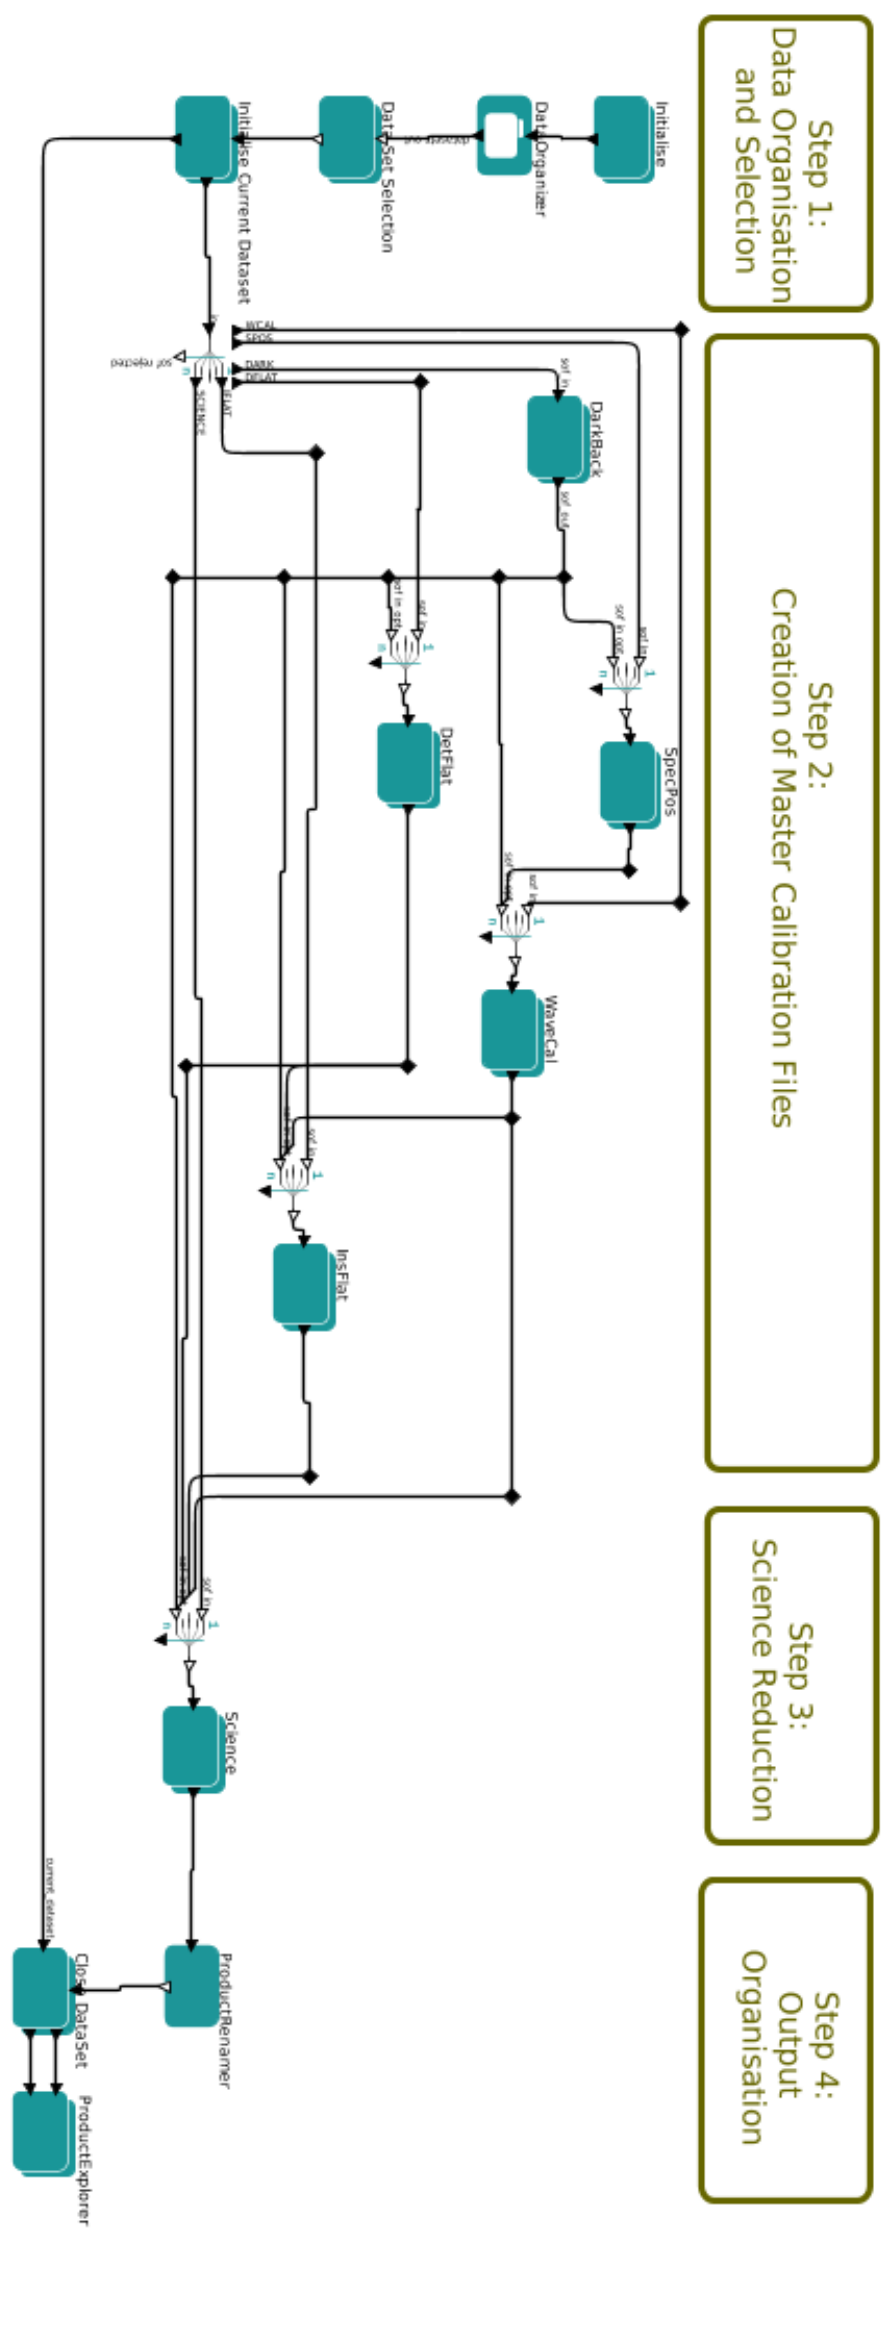
\includegraphics[height = 0.89\textheight]{workflow}%
\vspace{-2.5cm}
%\caption{}
%\label{fig:workf}
\end{figure}%
\end{document}